\chapter{SCI-HI Data Analysis}\label{Ch:Data}



\section{Preparing the Data}

Before the data can be analyzed for potential signals, it first has to go through an analysis pipeline to remove man-made RFI and instrumental noise and make the datasets easier to handle. 

\begin{figure}[htb]
\begin{center}
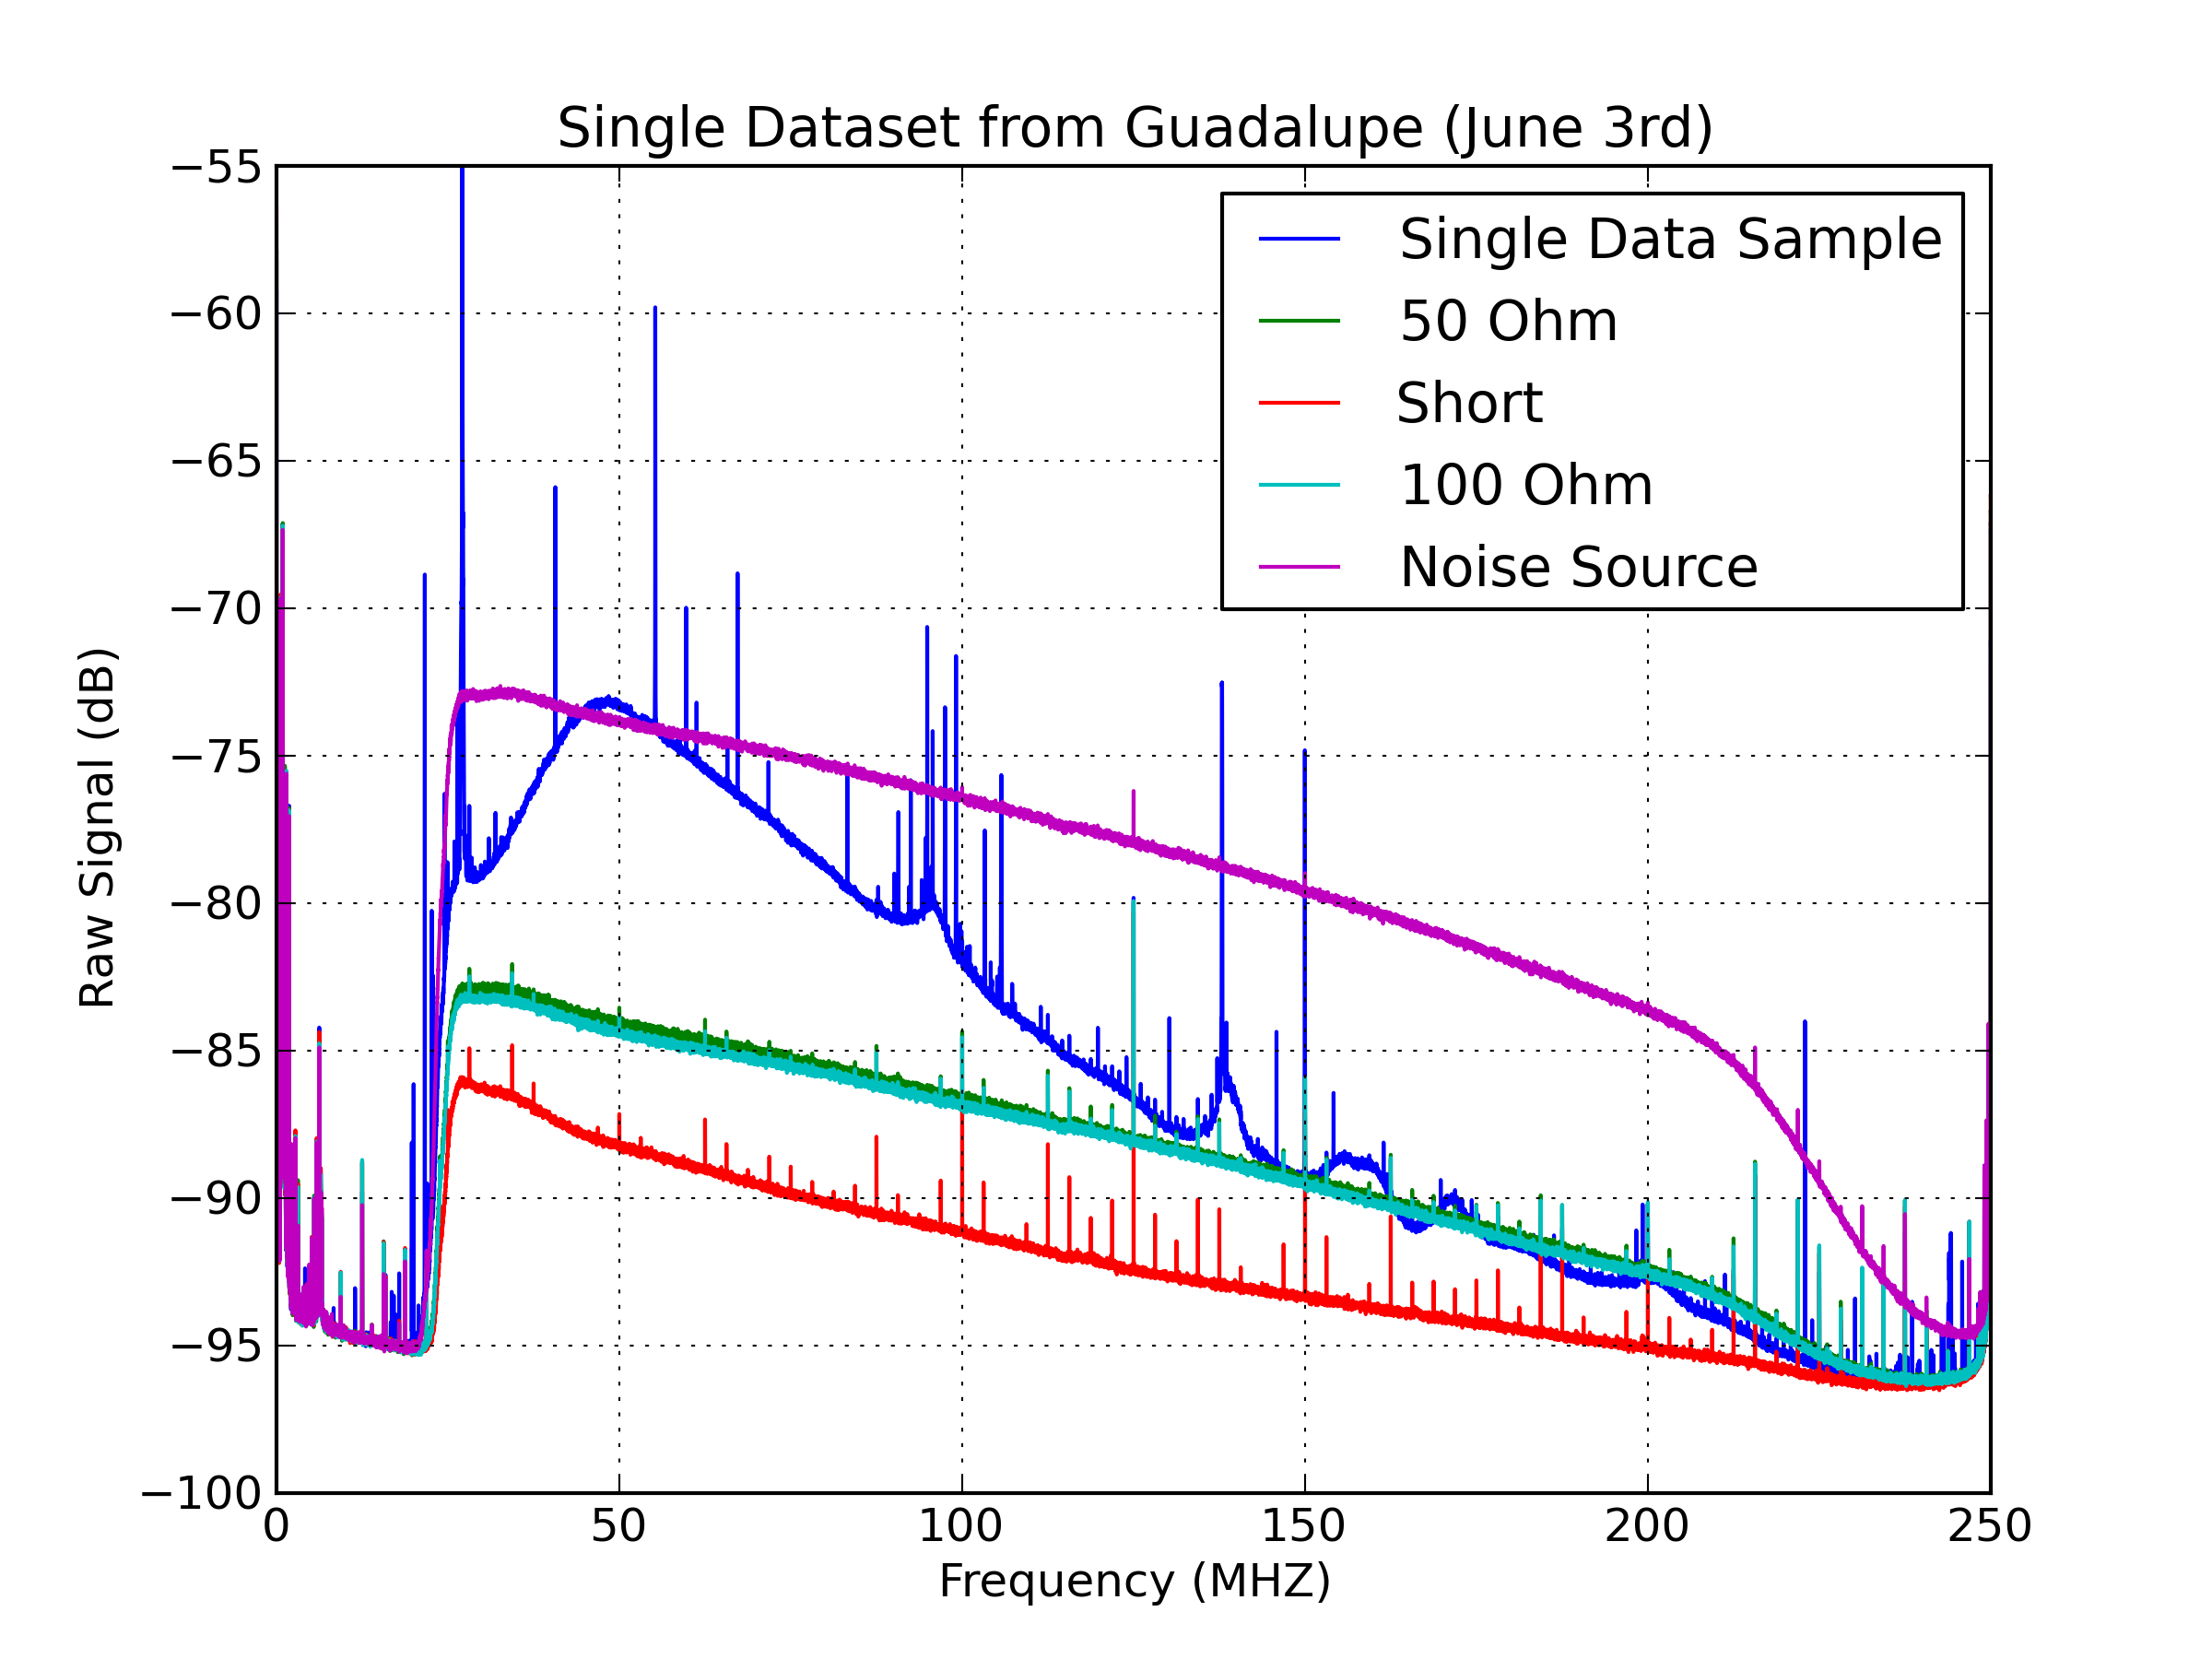
\includegraphics[width=0.88\linewidth]{Data_analysis/figures/single_raw_guad_june03.png}
\caption{Single dataset (1 second integration) of the entire frequency spectrum of raw data from the SCI-HI system. Also present are single datasets from the different calibration sources. }
\label{Fig:raw_data}
\end{center}
\end{figure}


\subsection{Integration and Sampling}\label{Sec:int}

The frequency spectrum collected for each second of data is stored in a single file with a header containing some basic information like the timestamp, DC voltage level (only collected when the system is powered by a DC Power Supply), system temperature, and switch position (antenna vs calibration sources). The spectrum covers the frequency range of 0-250 MHz, with a frequency resolution of $\sim 7.63$ kHz (or 32769 samples) and the data is stored in units of power (dB).

An example of the data collected by the system is shown in Figure \ref{Fig:raw_data}. Also included is a single sample of data from each of the calibration sources (Short, 50 $\Omega$, 100 $\Omega$, and Noise Source). 

Examining the data, we can identify several frequency dependent structures that are connected to the SCI-HI system design. The sharp signal dropoffs at 30 MHz and 200 MHz are caused by the high and low pass filters. The comb of narrow spikes present in both the antenna data and calibration data is due to the interleaved sampling strategy described in Section \ref{Sec:hard_split}. Long period frequency structures from 150-200 MHz are caused by the HIbiscus antenna beam and impedence. The $''$bump$''$ in the antenna data around 95 MHz is time-dependent and has been tied to the system power, so it is believed to be caused by RF leakage from the SCI-HI system. 

In addition, spikes present only in the antenna data are man-made RFI from beyond the SCI-HI system. These RFI spikes can be matched to RFI measured during site testing such as the FM band ($88-108$ MHz) and the orbcomm satellite band ($136-139$ MHz). 

Looking at the structure of the data over time, we can also see that the antenna data varies depending on what part of the sky it sees. This is shown in Figure \ref{Fig:raw_time_series}, where the daily variance of the single frequency is plotted.  


\begin{figure}[htb]
\begin{center}
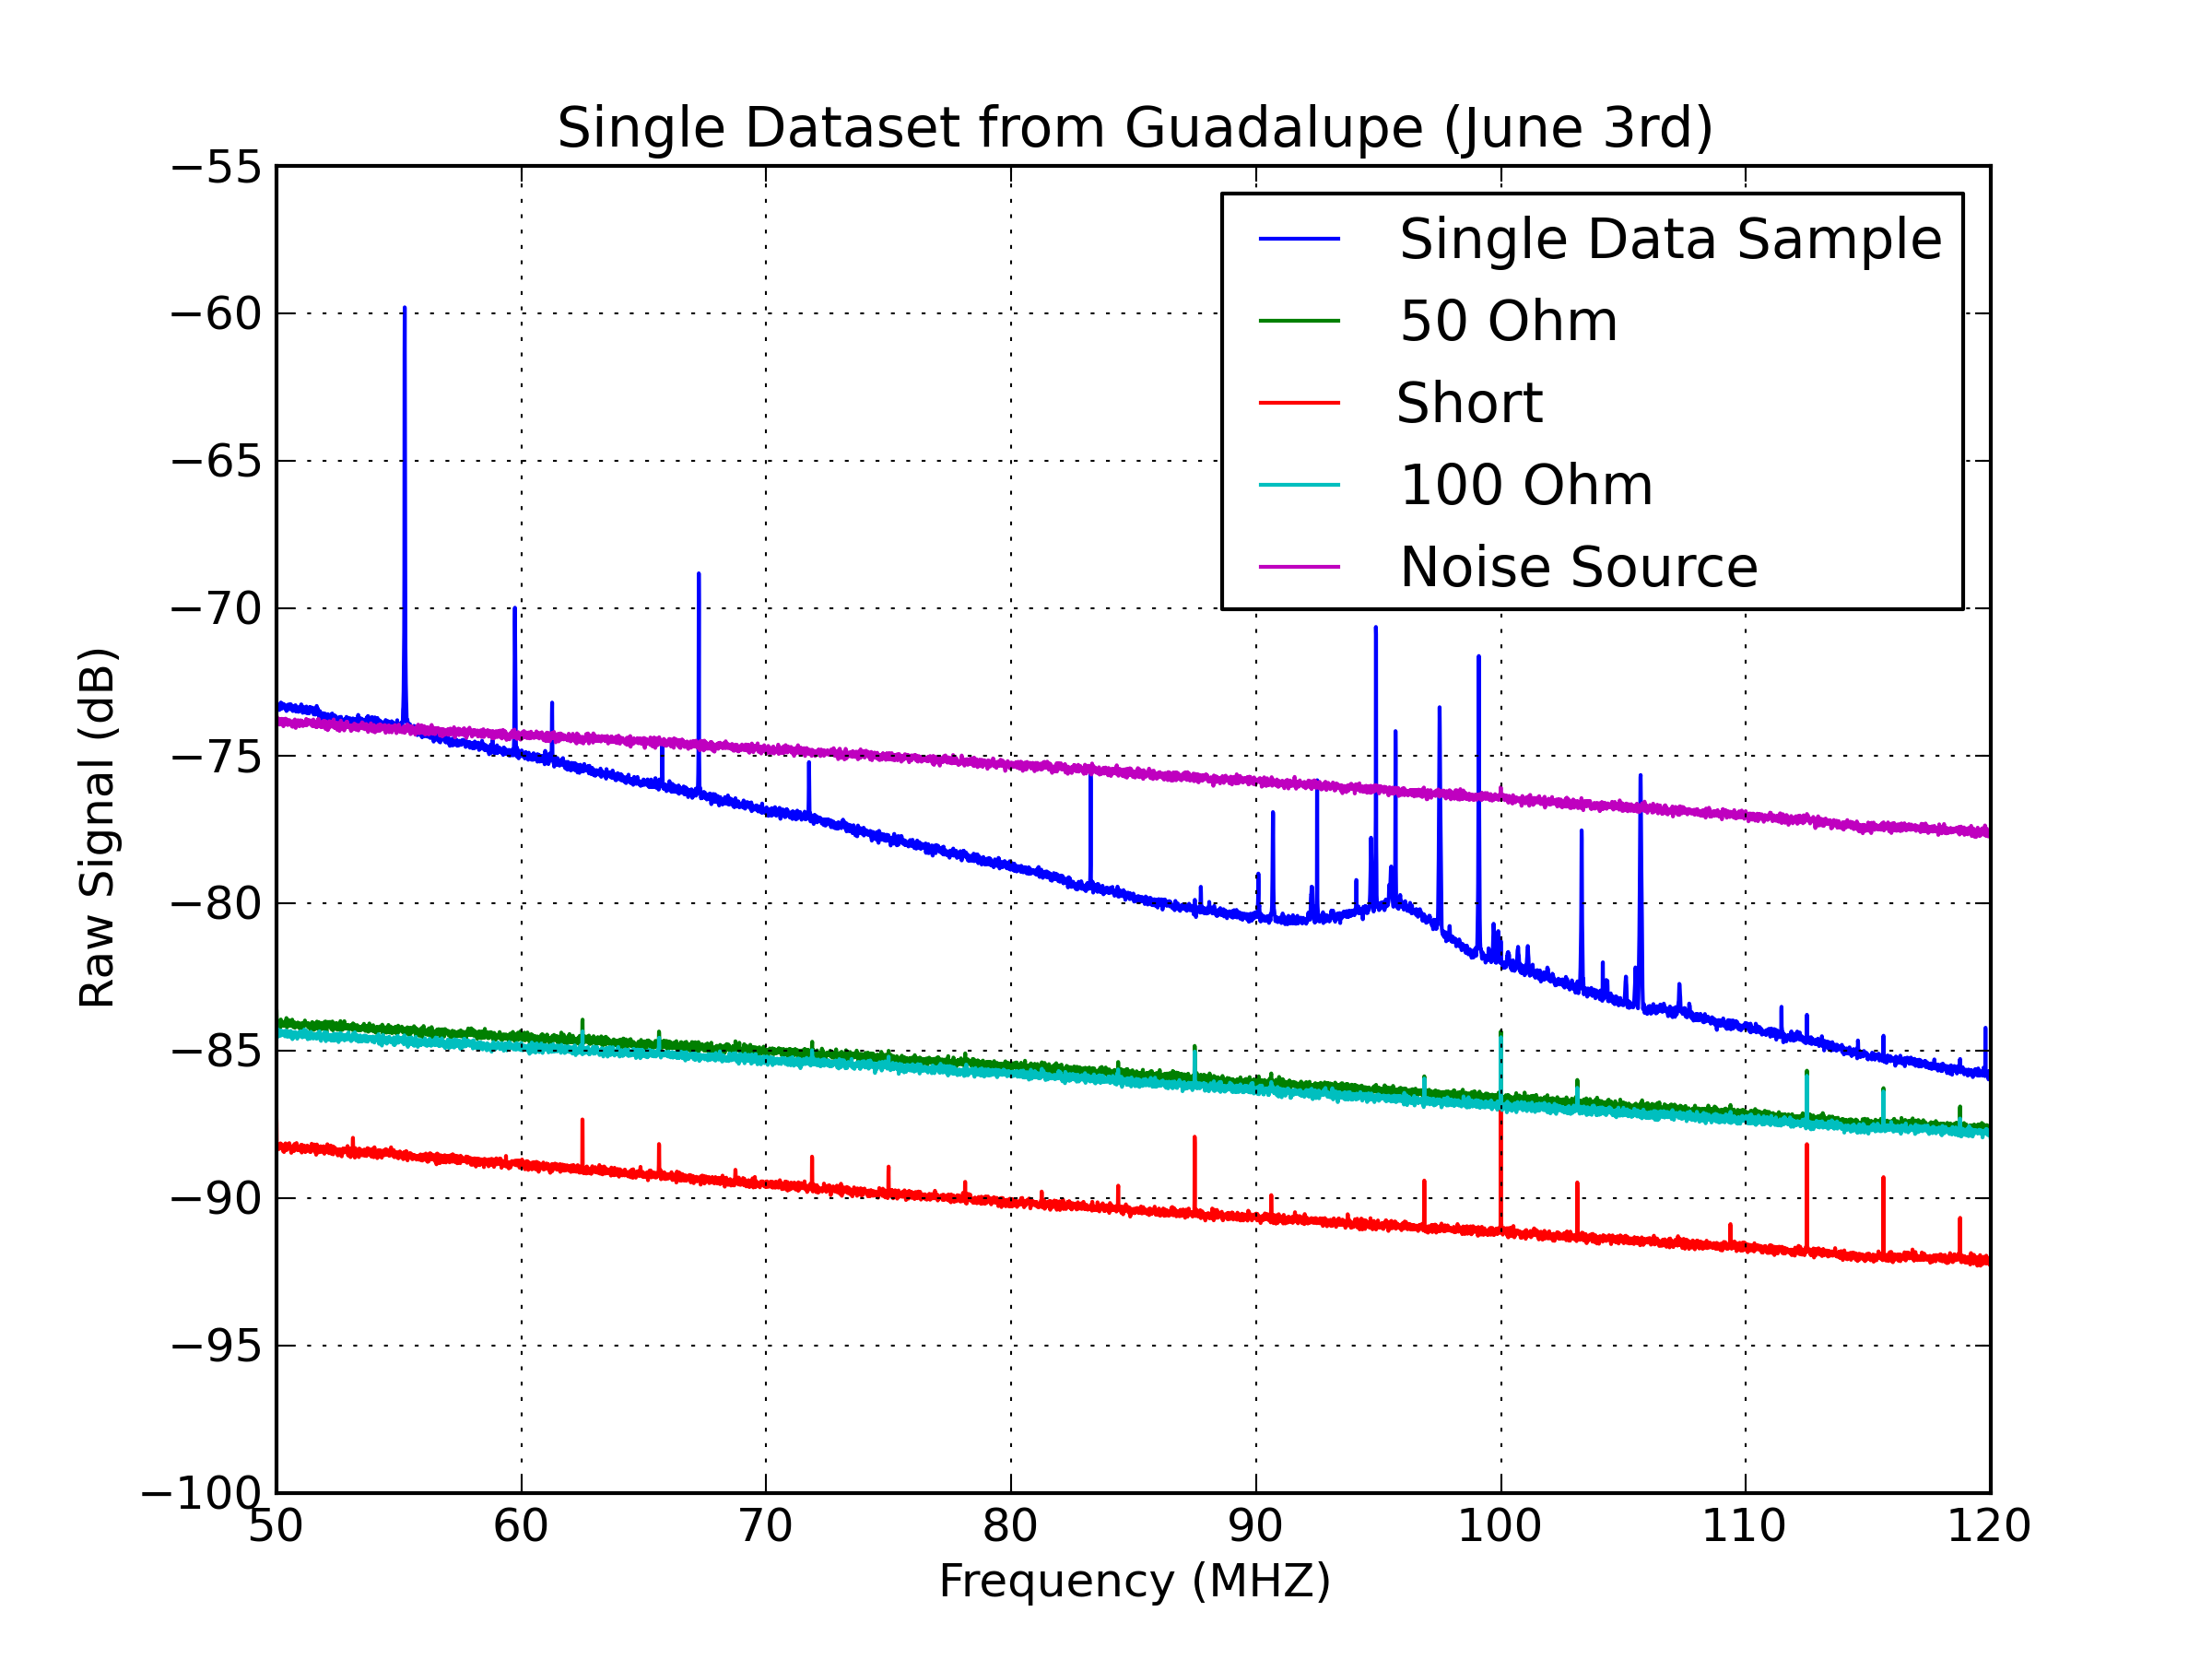
\includegraphics[width=0.9\linewidth]{Data_analysis/figures/single_raw_trunc_guad_june03.png}
\caption{Single dataset of a truncated spectrum of raw data from the SCI-HI system. Also present are single datasets from the different calibration sources.}
\label{Fig:raw_data_trunc}
\end{center}
\end{figure}


\subsection{Truncation}

Because the data we are interested in is a subset of the overall spectrum, one of the first things that we can do is to truncate frequency range of the data to make it smaller. We can throw away data for frequencies where the HIbiscus antenna doesn't have a stable beam or the data is dominated by signals other than those from the sky. 

In the 2013 data, the reliable band corresponds to (50-120 MHz), as is shown in Figure \ref{Fig:raw_data_trunc}. In this part of the spectrum, the linear slope of the antenna dataset compared to the calibration datasets stands out. This linear slope is caused by the spectrum of synchrotron radiation in the Milky Way Galaxy, as will be discussed in later sections of this chapter. 


\subsection{RFI Excision}

Another early stage of the pipeline is RFI excision (both in frequency and time) of narrow features or spikes in the data. 

\subsubsection{RFI Frequency Flagger}

RFI excision in frequency is done by flagging each dataset according to a threshold. The threshold is calculated for each frequency ($f_c$) in the spectrum by fitting a small subset of the spectrum ($f_c-n \leq f \leq f_c + n$), where $n$ is the number of nearest neighbors used for the fit. This fit is a two term polynomial. 

Dividing out the fit gives a flattened dataset whose mean is one and whose variance can be calculated. The variance is used to set a threshold (eg $3 \sigma$), and if the flattened data at $f_c$ is outside the threshold then $f_c$ is flagged. 

Flagging identifies a list of frequencies between $50-120$ MHz which have a spike above the threshold in a given dataset. 

The exact threshold and number of neighbors used to set the mean can be tweaked, but the typical values I used were a 3$\sigma$ threshold and 32 neighbors on either side. If a data point is flagged, it is masked out of the data and will not be included in further analysis.  

\begin{figure}[htb]
\begin{center}
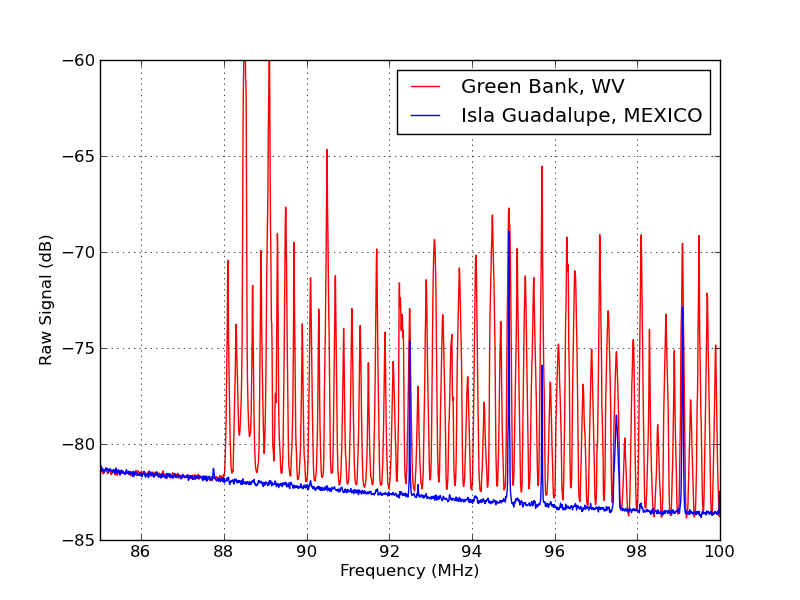
\includegraphics[width=0.9\linewidth]{Data_analysis/figures/FM_band_comp.png}
\caption{RFI comparison in the FM band between Isla Guadalupe and Green Bank, West Virginia. }
\label{Fig:FM_band}
\end{center}
\end{figure}

\subsubsection{RFI in the FM Band}

One of the frequency bands where RFI excision is particulary challenging is in the FM band (88-108 MHz). In this band, the variance of the signal can be quite large; making the RFI excision procedure less reliable. For many of our testing sites like Green Bank, WV the entire FM band is occupied with large RFI signals (as discussed in Chapter \ref{Ch:RFI}). This can be seen in Figure \ref{Fig:FM_band}, where the RFI signals are on average $\sim$10 dB above the floor. 

On the other hand, the FM band RFI signals from Isla Guadalupe are mostly $\leq$1 dB. These RFI signals are small enough to be missed by the RFI flagger and may be run through the rest of the pipeline stages. The few large spikes $\geq$5 dB above the floor will be removed by the RFI excision code. 

\begin{figure}[htb]
\begin{center}
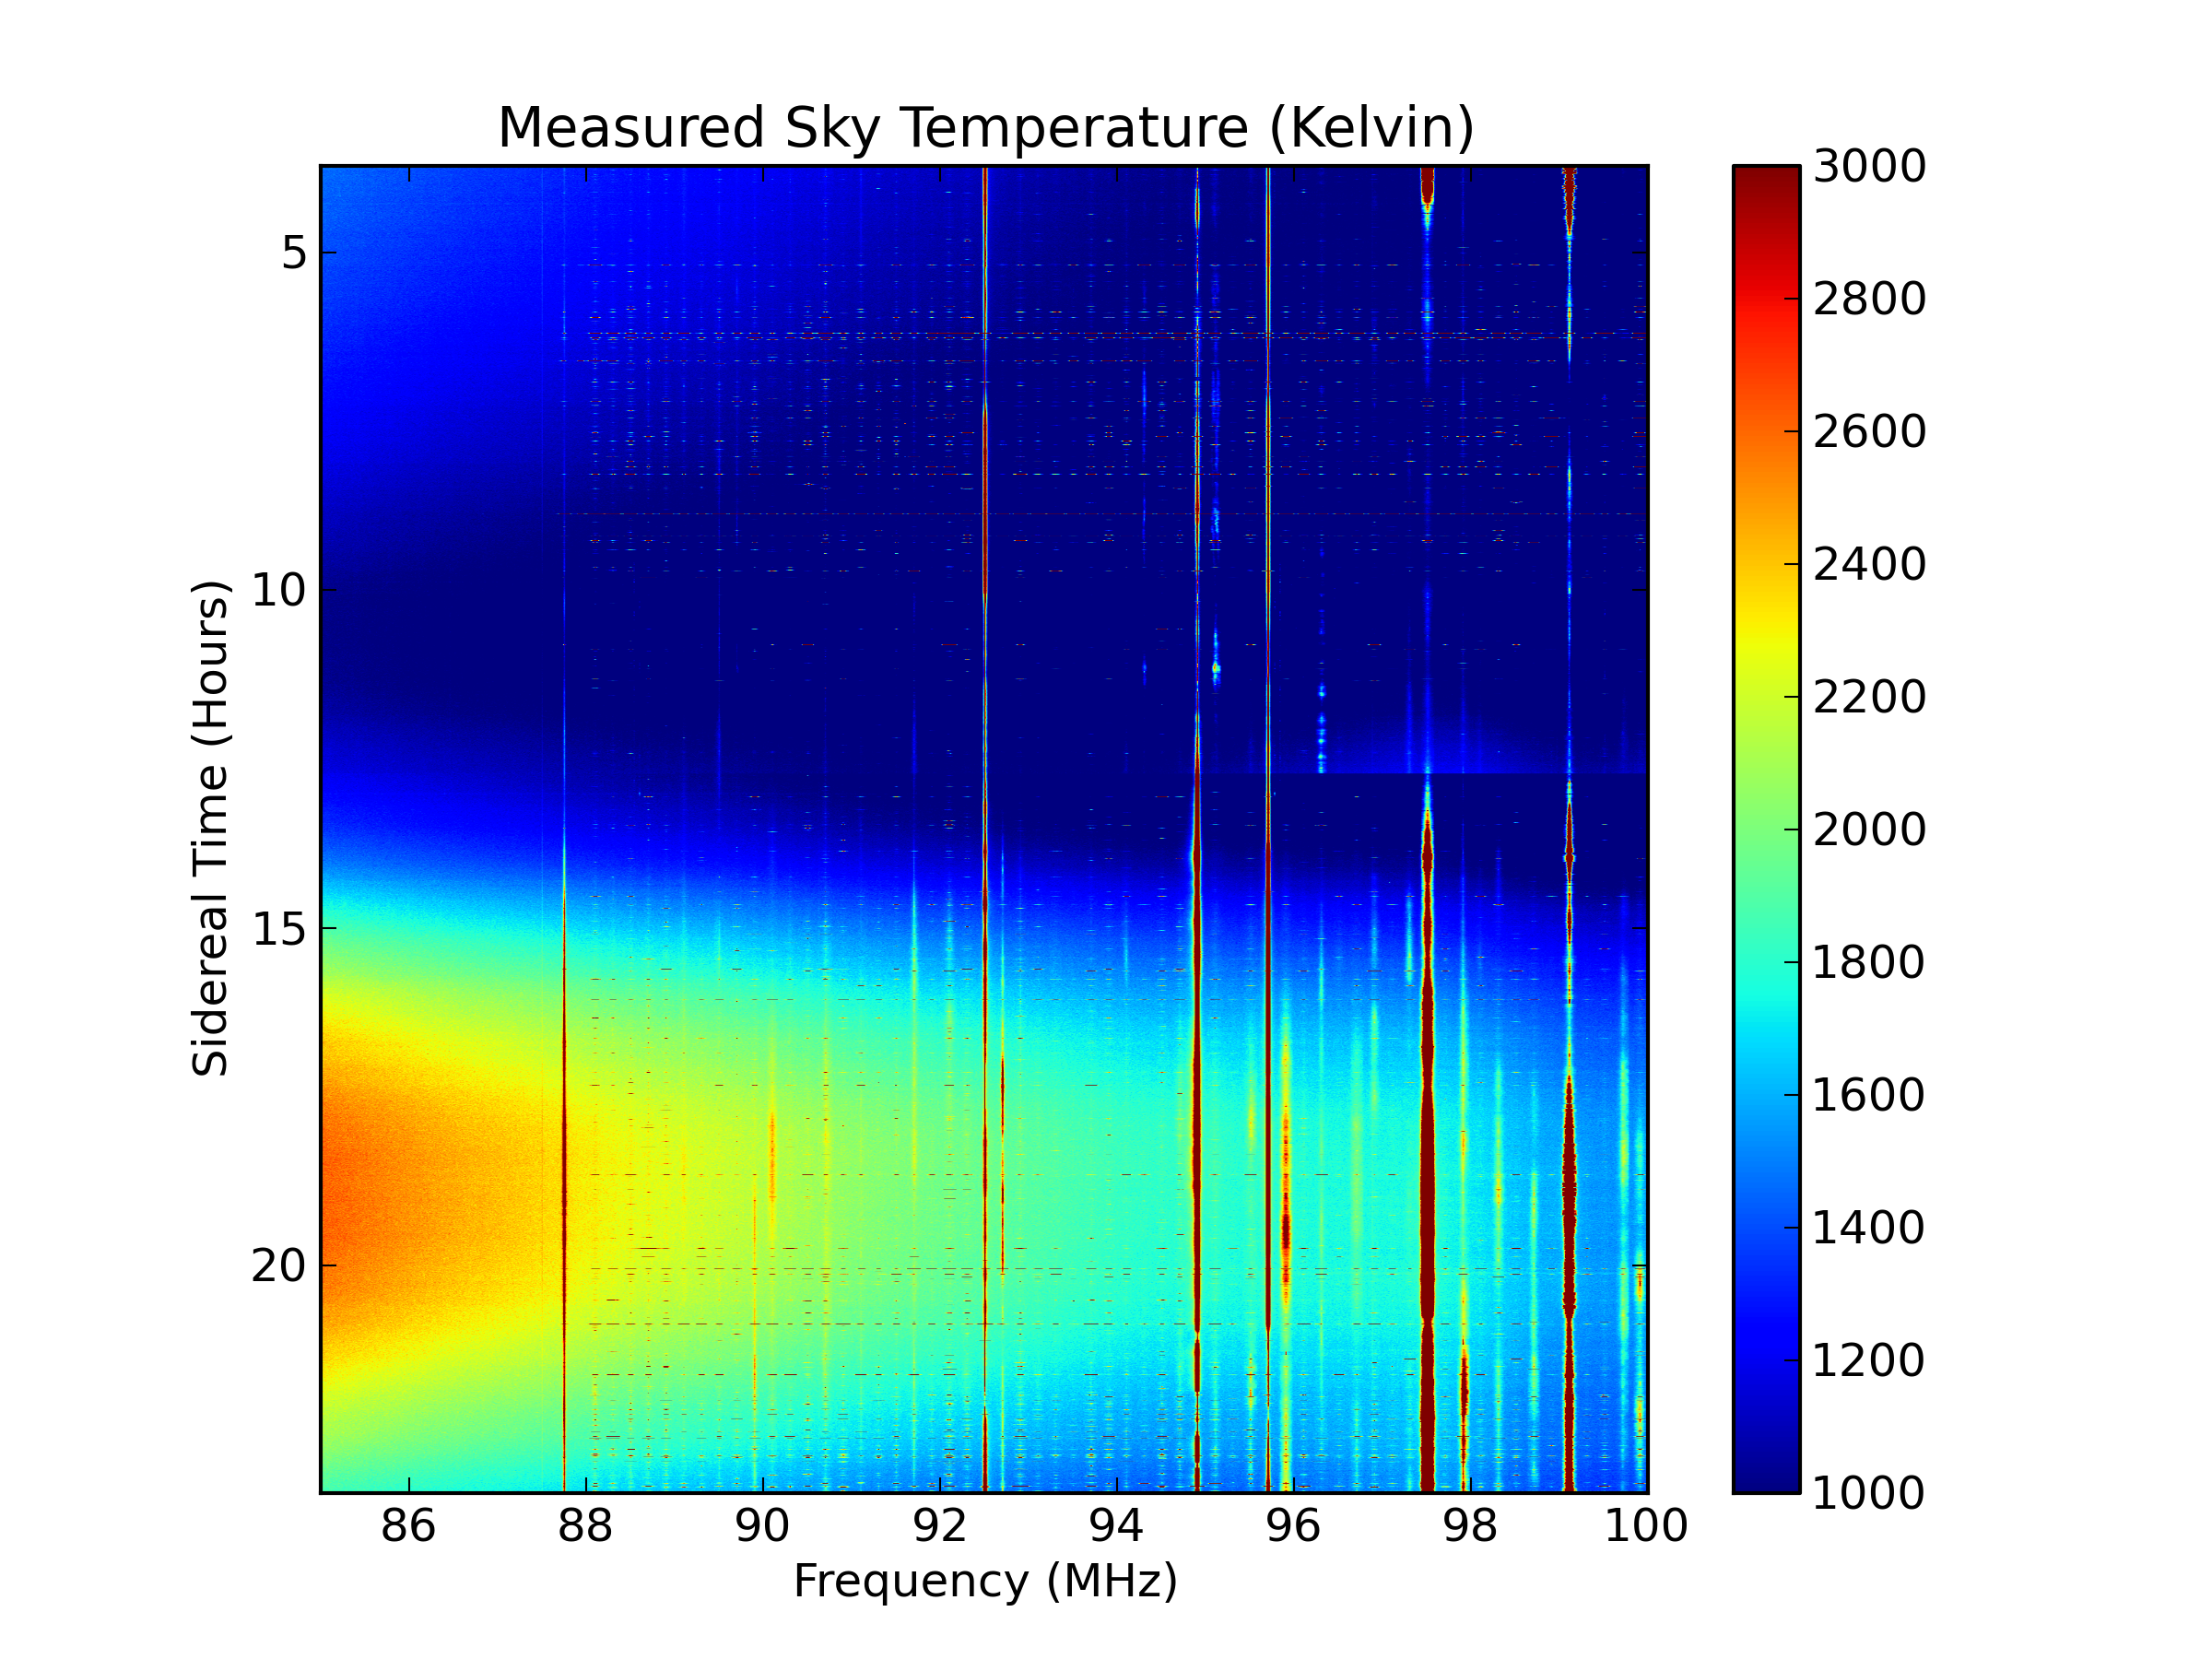
\includegraphics[width=0.9\linewidth]{Data_analysis/figures/June_06_unmasked_cal_waterfall_FM.png}
\caption{Calibrated full day of data taken on June 6th, 2013 showing RFI variance for 85-100 MHz. Note that the vertical lines correspond to FM stations, while horizontal lines correspond to times of meteor activity. }
\label{Fig:RFI_wf_long}
\end{center}
\end{figure}

\begin{figure}[htb]
\centering
\begin{minipage}[b]{0.48\textwidth}
\centering
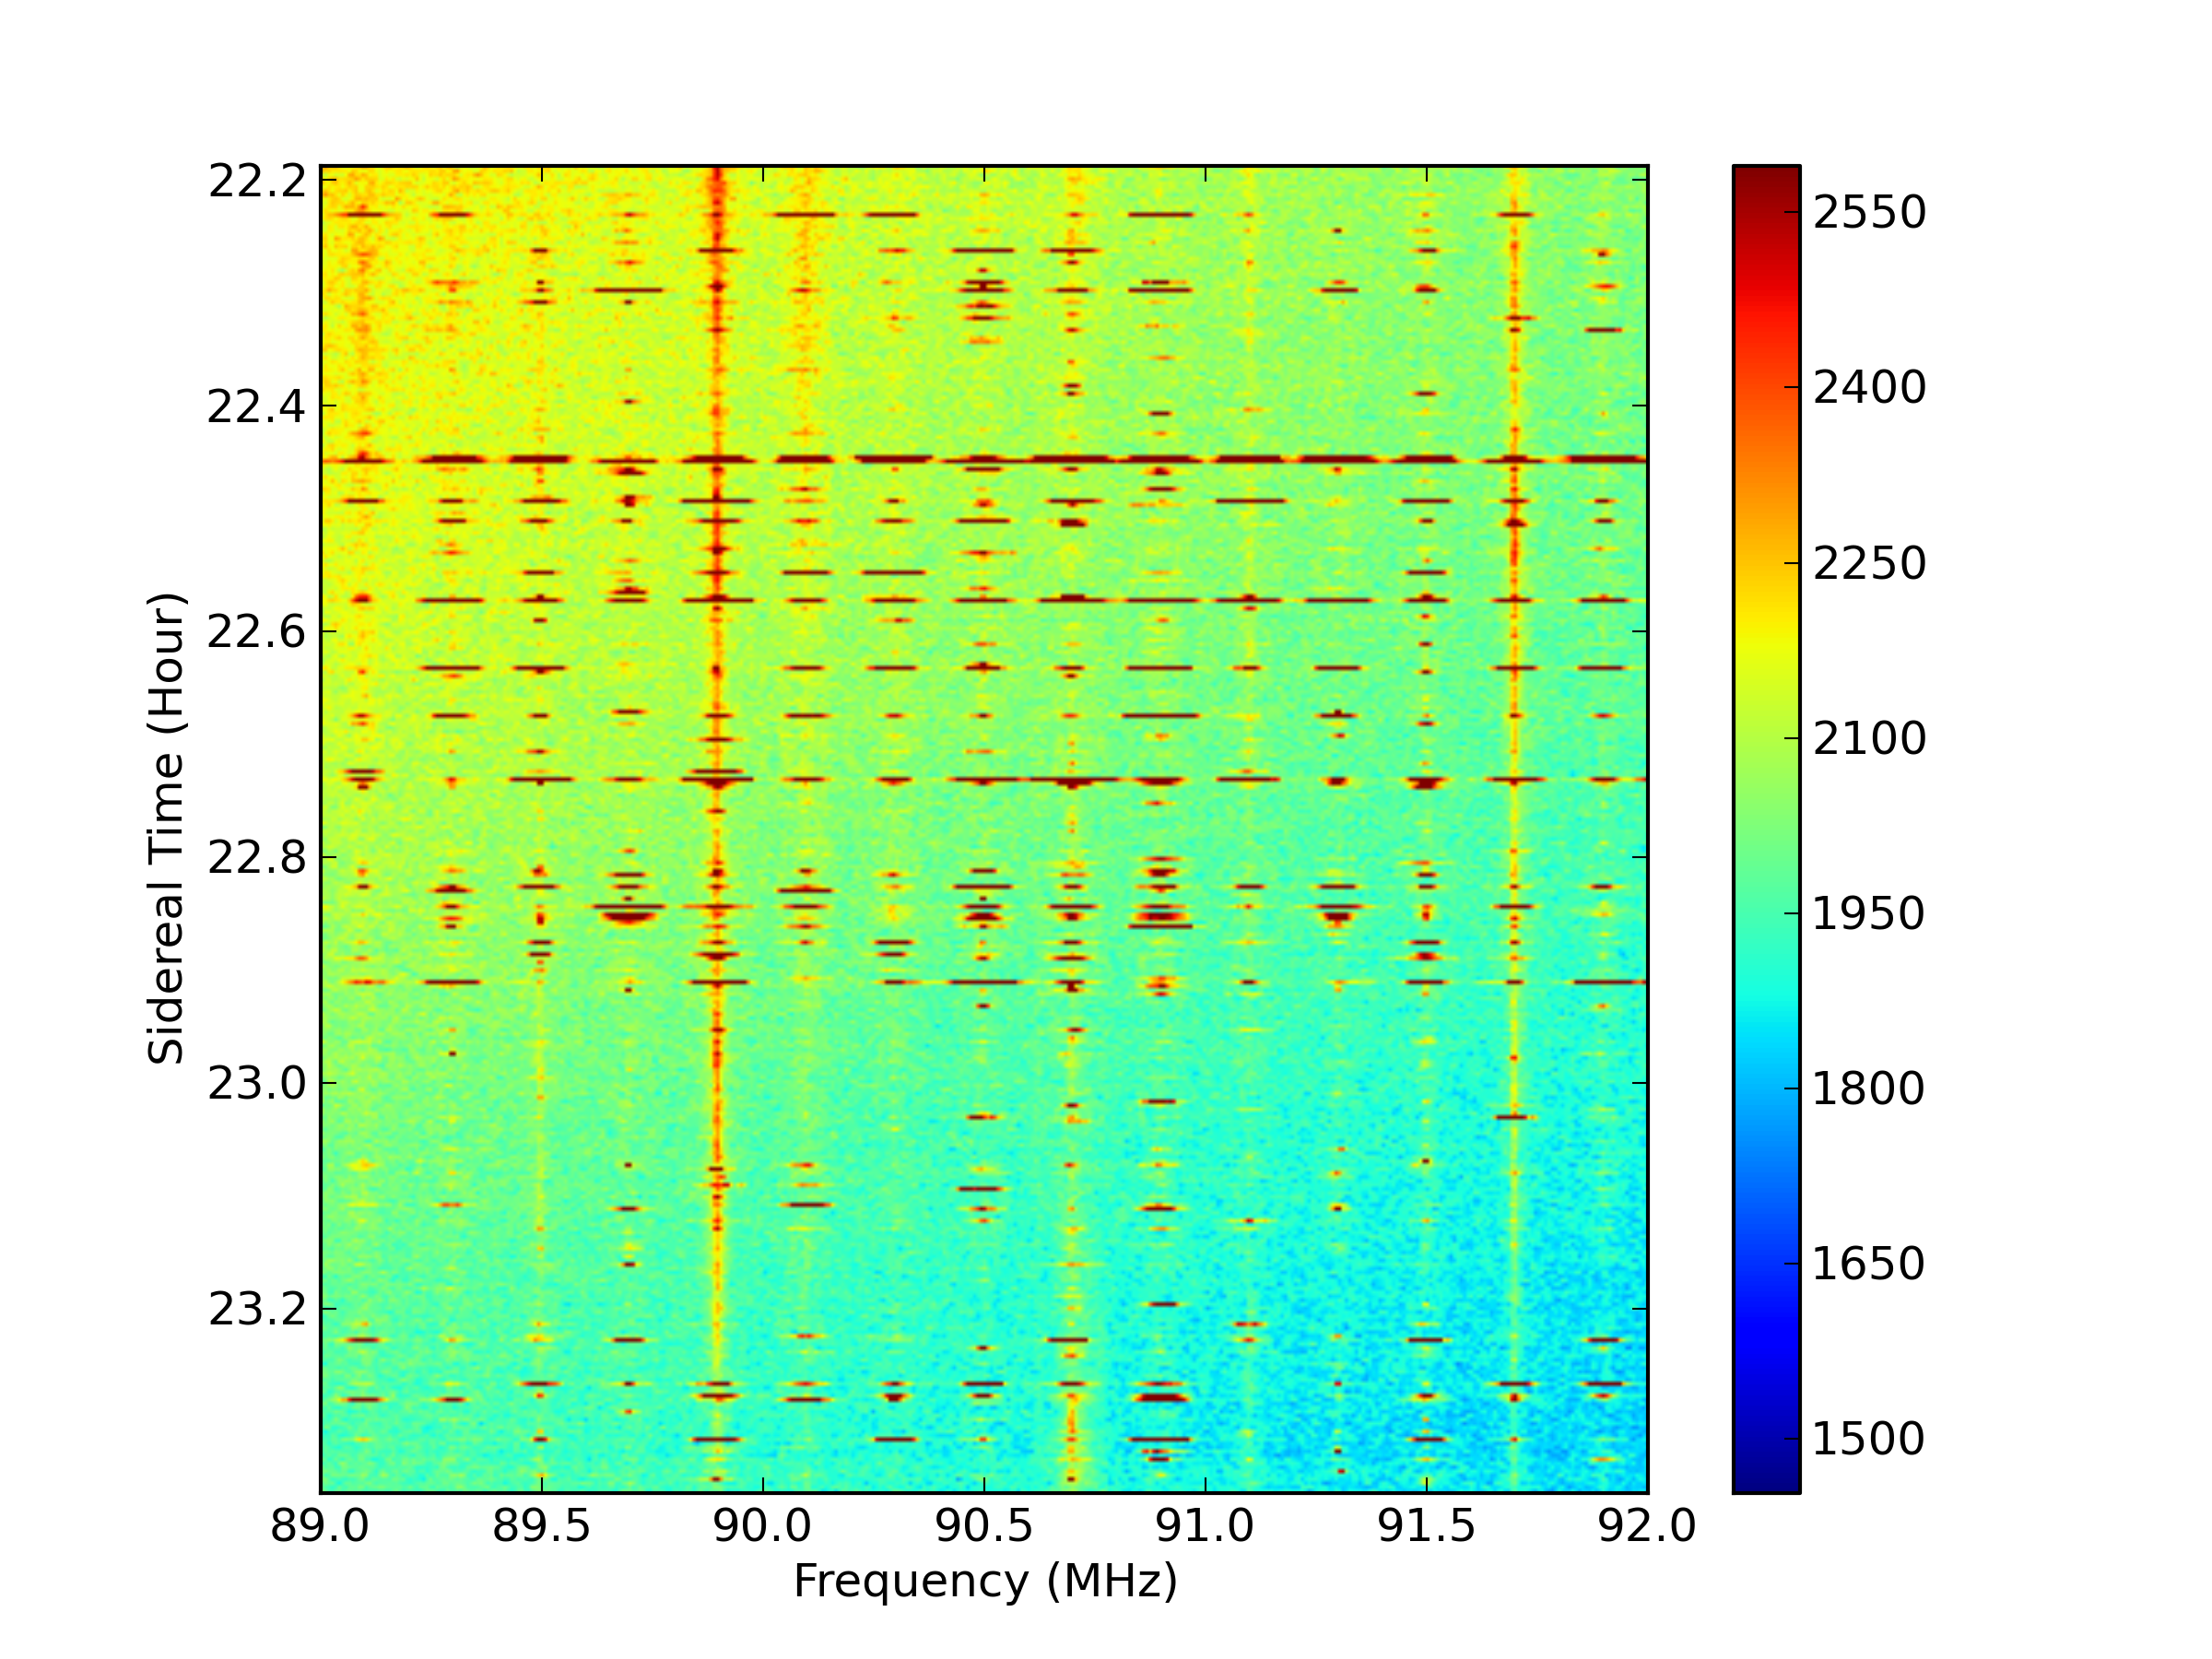
\includegraphics[width=0.95\linewidth]{Data_analysis/figures/June_06_part_13_unmasked_FM_waterfall.png}
\caption{Short ($\sim1$ hour) subset of data taken on June 6th, 2013. Data shows RFI variance for 89-92 MHz during a period of high meteor activity. }
\label{Fig:RFI_wf_short_full}
\end{minipage}%
\begin{minipage}[b]{0.02\textwidth}
\hspace{1cm}
\end{minipage}%
\begin{minipage}[b]{0.48\textwidth}
\centering
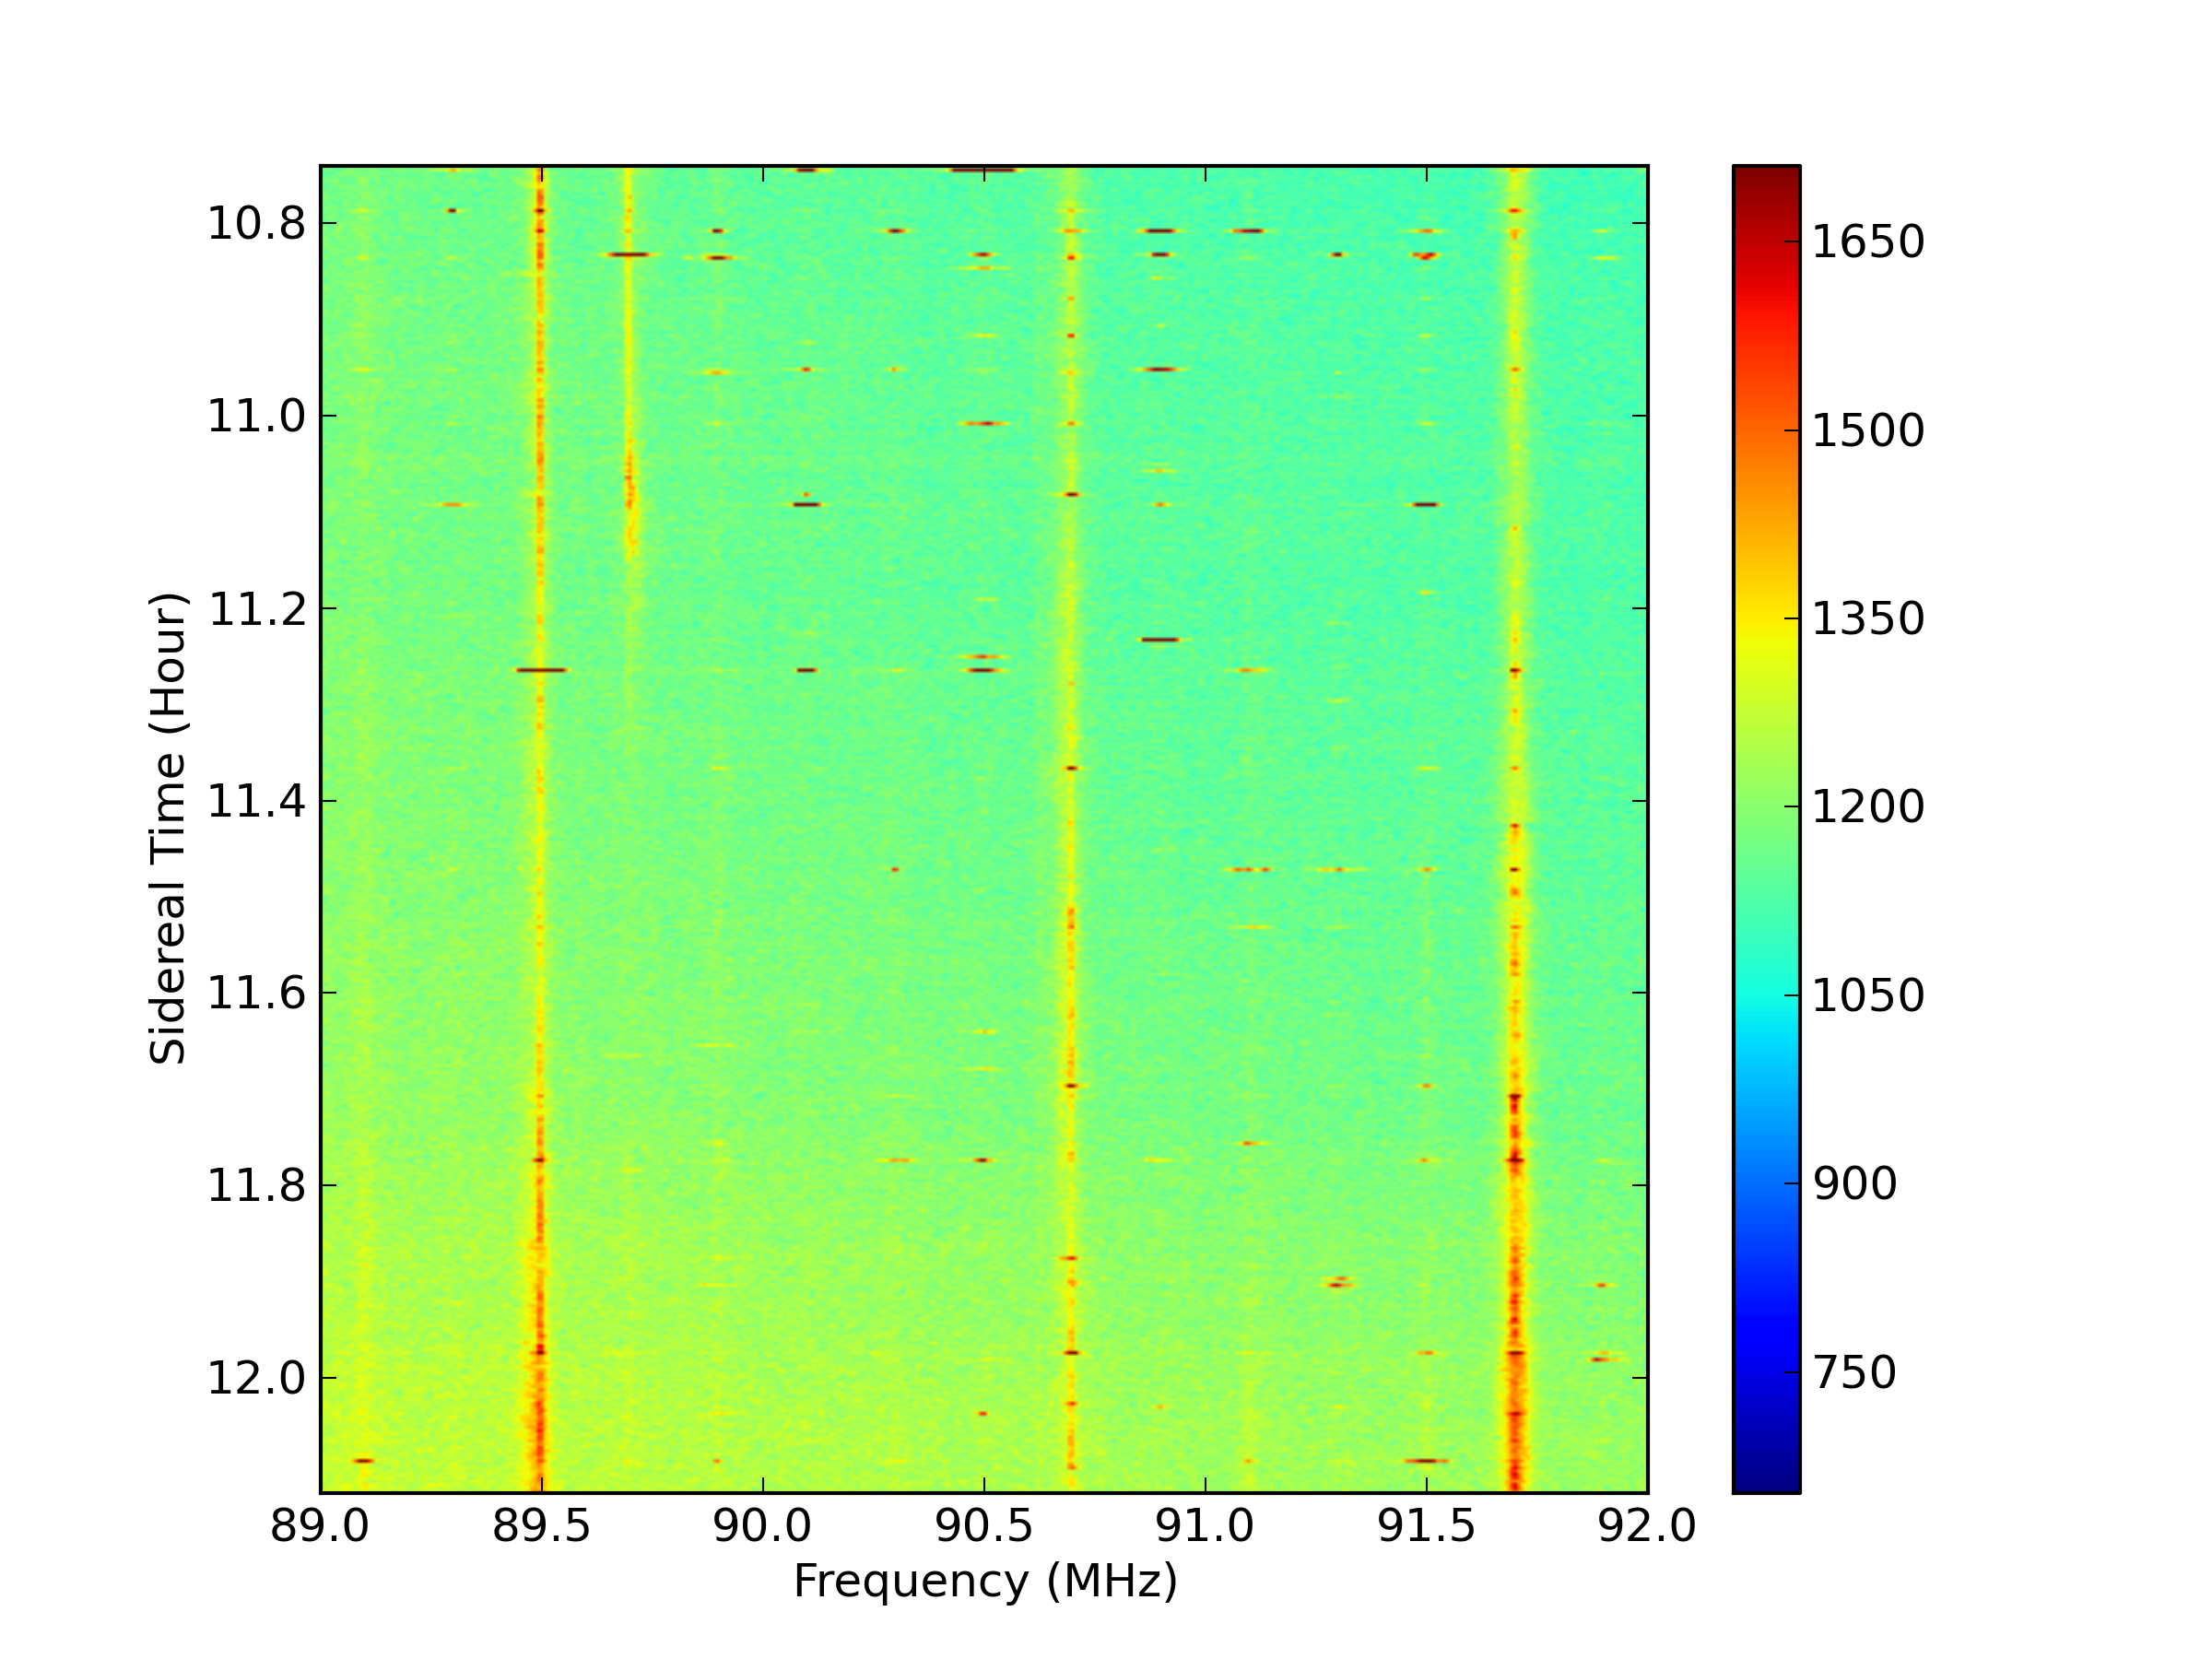
\includegraphics[width=0.95\linewidth]{Data_analysis/figures/June_06_part_5_unmasked_FM_waterfall.png}
\caption{Short ($\sim1$hr) subset of data taken on June 6th, 2013. Data shows RFI variance for 89-92 MHz during a period of low meteor activity.}
\label{Fig:RFI_wf_short_empty}
\end{minipage}
\end{figure}

\subsubsection{Time-variable RFI}

While most of the RFI in the data is time independent and can be flagged out in each dataset indpendently, some of the RFI has a strong time-dependence. 

\paragraph{Time-variability of RFI due to Meteor Scatter}

Meteoroids are always passing through Earth's atmosphere. These meteoroids have a wide spectrum of sizes starting from $\leq$10 nm. As these meteoroids pass through the earth's atmosphere, some of their atoms are vaporized. Inelastic collisions between these atoms and air molecules in the atmosphere can lead to ionization \cite{meteor_review}. 

The result of this ionization is an increase in the column density of free electrons  in the Earth's ionosphere along the meteor trail. This temporarily increases the plasma frequency of the ionosphere along that trail, such that the ionosphere is opaque at higher frequencies along the trail. This opacity allows reflection of signals such as FM radio off the ionosphere, extending the range of visibility for the FM band beyond what would normally be accessible.

In the SCI-HI data, this leads to a time-variable increase in the FM band RFI. For short time periods the strength of RFI signals from FM radio towers becomes larger. The duration of these signals is relatively small, typically lasting only a few seconds and diminishing as free electrons diffuse away from the original meteor trail. 

The magnitude of the increase in the FM signals is also variable, and different RFI signals are amplified depending on the location of the meteor trail. Meteor amplification of RFI is highly time variable, as meteors don't fall evenly, but rather travel in groups (aka meteor showers). Also, smaller meteoroids produce smaller trails, which allow for less transmission of FM signals.

This can be seen in looking at Figure \ref{Fig:RFI_wf_long}, which shows half of the FM band over one day of data collection. In this waterfall plot, strong FM stations are seen as vertical lines, while meteor scatter events show up as horizontal lines. When we zoom in, as in Figures \ref{Fig:RFI_wf_short_full} and \ref{Fig:RFI_wf_short_empty}, we can see differences in meteor scatter rate and metor trail size.

\paragraph{Time-variability of RFI from Local Sources}

Another source of time-variable RFI is local noise from the surroundings. Our site at Isla Guadalupe was a few km from the local fishing village, which meant that occasionally RFI was picked up from the village when the diesel generator was powered on during the day. Additionally, the site was a few hundred meters from the road that led from the village to the rest of the island. When vehicles drove past the site (a few times each day), RFI from the vehicles such as broad band RF from spark plugs could be seen in the data. 

\subsubsection{Time-variable RFI Flagging}

In order to remove such time-variable RFI, I wrote a second RFI flagger identical to the frequency flagger, except that it works along the time axis. I typically used the same threshold and number of neighbors as the frequency flagger. 


\subsection{Rebinning}

Because the data is collected at a much higher resolution than is needed for the analysis, it needs to be rebinned to lower resolution. This can be done either in frequency or time. Compression is done after RFI flagging in order to keep a single $''$bad$''$ channel from affecting the overall signal. The mean of the unflagged data for a given bin scale becomes the new data point. In addition, a new data point is left as a flagged point if over half of the data used to make it were flagged. 



\section{Calibrating the Data}

After RFI removal and compression, the data is ready for calibration. Calibration is used both to put the data into correct units and also remove instrumental structure in the frequency spectra. 


\subsection{Calibration Datasets} \label{Sec:calsource}

Part of the SCI-HI system, as laid out in Chapter \ref{Ch:System}, is an electro-mechanical switch that allows data collection from both the antenna and known temperature sources placed on the different switch input terminals. Figures \ref{Fig:raw_data} and \ref{Fig:raw_data_trunc} show the different datasets measured with the system, which are also known as $''$Johnson Noise$''$ datasets. 

In these datasets, the temperature of each source can be separated into different terms. 

\paragraph{Short Terminator}

For the $''$Short$''$ signal, a shorting terminator is placed on the switch input terminal. This means that all of the signal seen in the data processor is coming from the SCI-HI system. This includes both instrumental noise and thermal noise. Therefore, we'll call the instrumental noise power $P_{short}$.

\paragraph{$50 \Omega$ Terminator}

For the $'' 50 \Omega ''$ signal, a load is placed on the switch input with an impedance of $50 \Omega$. The load provides an input of the current ambient temperature, and instrumental and termal noise adds additional signal. There is an another noise term ($P_Z$), which depends on the match between the impedence of the first stage amplifier and the load. So, we can write the $50 \Omega$ power as:

\begin{equation}
P_{50 \Omega} = P_{amb}+P_{Z50}+P_{short}+P_{thermal}
\end{equation}

\paragraph{$100 \Omega$ Terminator}

For the $'' 100 \Omega ''$ signal, a load is placed on the switch input with an impedance of $100 \Omega$. This load provides a nearly identical power as the $50 \Omega$ load, with the exception of the impedance term. So, we can write the $100 \Omega$ power as:

\begin{equation}
P_{100 \Omega} = P_{amb}+P_{Z100}+P_{short}+P_{thermal}
\end{equation}

\paragraph{Artificial Noise Source}

For the $''$Noise Source$''$ signal, an artificial noise source with $50 \Omega$ impedance is placed on the switch input. This source provides both an ambient temperature signal and an additional artificial noise signal ($P_{Noise}$) which can be independently measured. The impedance noise term matches the $50 \Omega$ impedance term. So, we can write the noise source power as:

\begin{equation}
P_{NS} = P_{Noise} + P_{amb}+P_{Z50}+P_{short} +P_{thermal}
\end{equation}


\paragraph{Antenna}

For the signal from the HIbiscus antenna, we can write a similar equation for the power. In this case, we have thermal and instrument noise and an impedance term, as well as signals from the sky. 

\begin{equation}\label{Eq:T_ant}
P_{Ant} = P_{sky}+P_{Zant}+P_{short} + P_{thermal}
\end{equation}

\paragraph{Impedance (current) Noise} 

The impedance noise ($P_Z$) is also called the current noise of the system. To understand this definition, we go back to the basic circuit diagram of an amplifier. If the amplifier input is hooked up to a short, the measured noise in units of power is $P \propto V^2$, where V is the voltage sent into the amplifier. 

On the other hand, when the $50 \Omega$ (or $100 \Omega$) terminator is connected the additional noise present in the system beyond the short noise also has a voltage. The magnitude of this voltage is $V\propto I Z$, where $I$ is the current through the system and $Z$ is the impedance of the terminator \cite{stutzman1981}.

Given Figure \ref{Fig:raw_data}, which shows that $P_{50 \Omega} \cong P_{100 \Omega}$ while $Z_{100 \Omega} = 2 Z_{50 \Omega}$, the current noise term must be small for our system. For the remainder of the analysis, we will assume that $T_Z = 0$ for both the calibration data and the antenna data. 


\subsection{On-site Impedance Measurement}

Impedance can be measured using a Vector Network Analyzer (VNA) looking at the reflectivity (S11) data for the input sources. The calibration sources have an impedance that is constant in frequency ($50 \Omega$ or $100 \Omega$) and has zero complex phase.

In comparison, the HIbiscus antenna has a complex impedance that varies with frequency and has a phase component (see Section \ref{Sec:HIbiscus_Imp} and Figures \ref{Fig:HIS11_dB_70} and \ref{Fig:HIS11_Smith_70}). This impedance must be measured in-situ, since it can depend on the exact layout of the system and the shape of the terrain around the antenna. 

\begin{figure}[htb]
\begin{center}
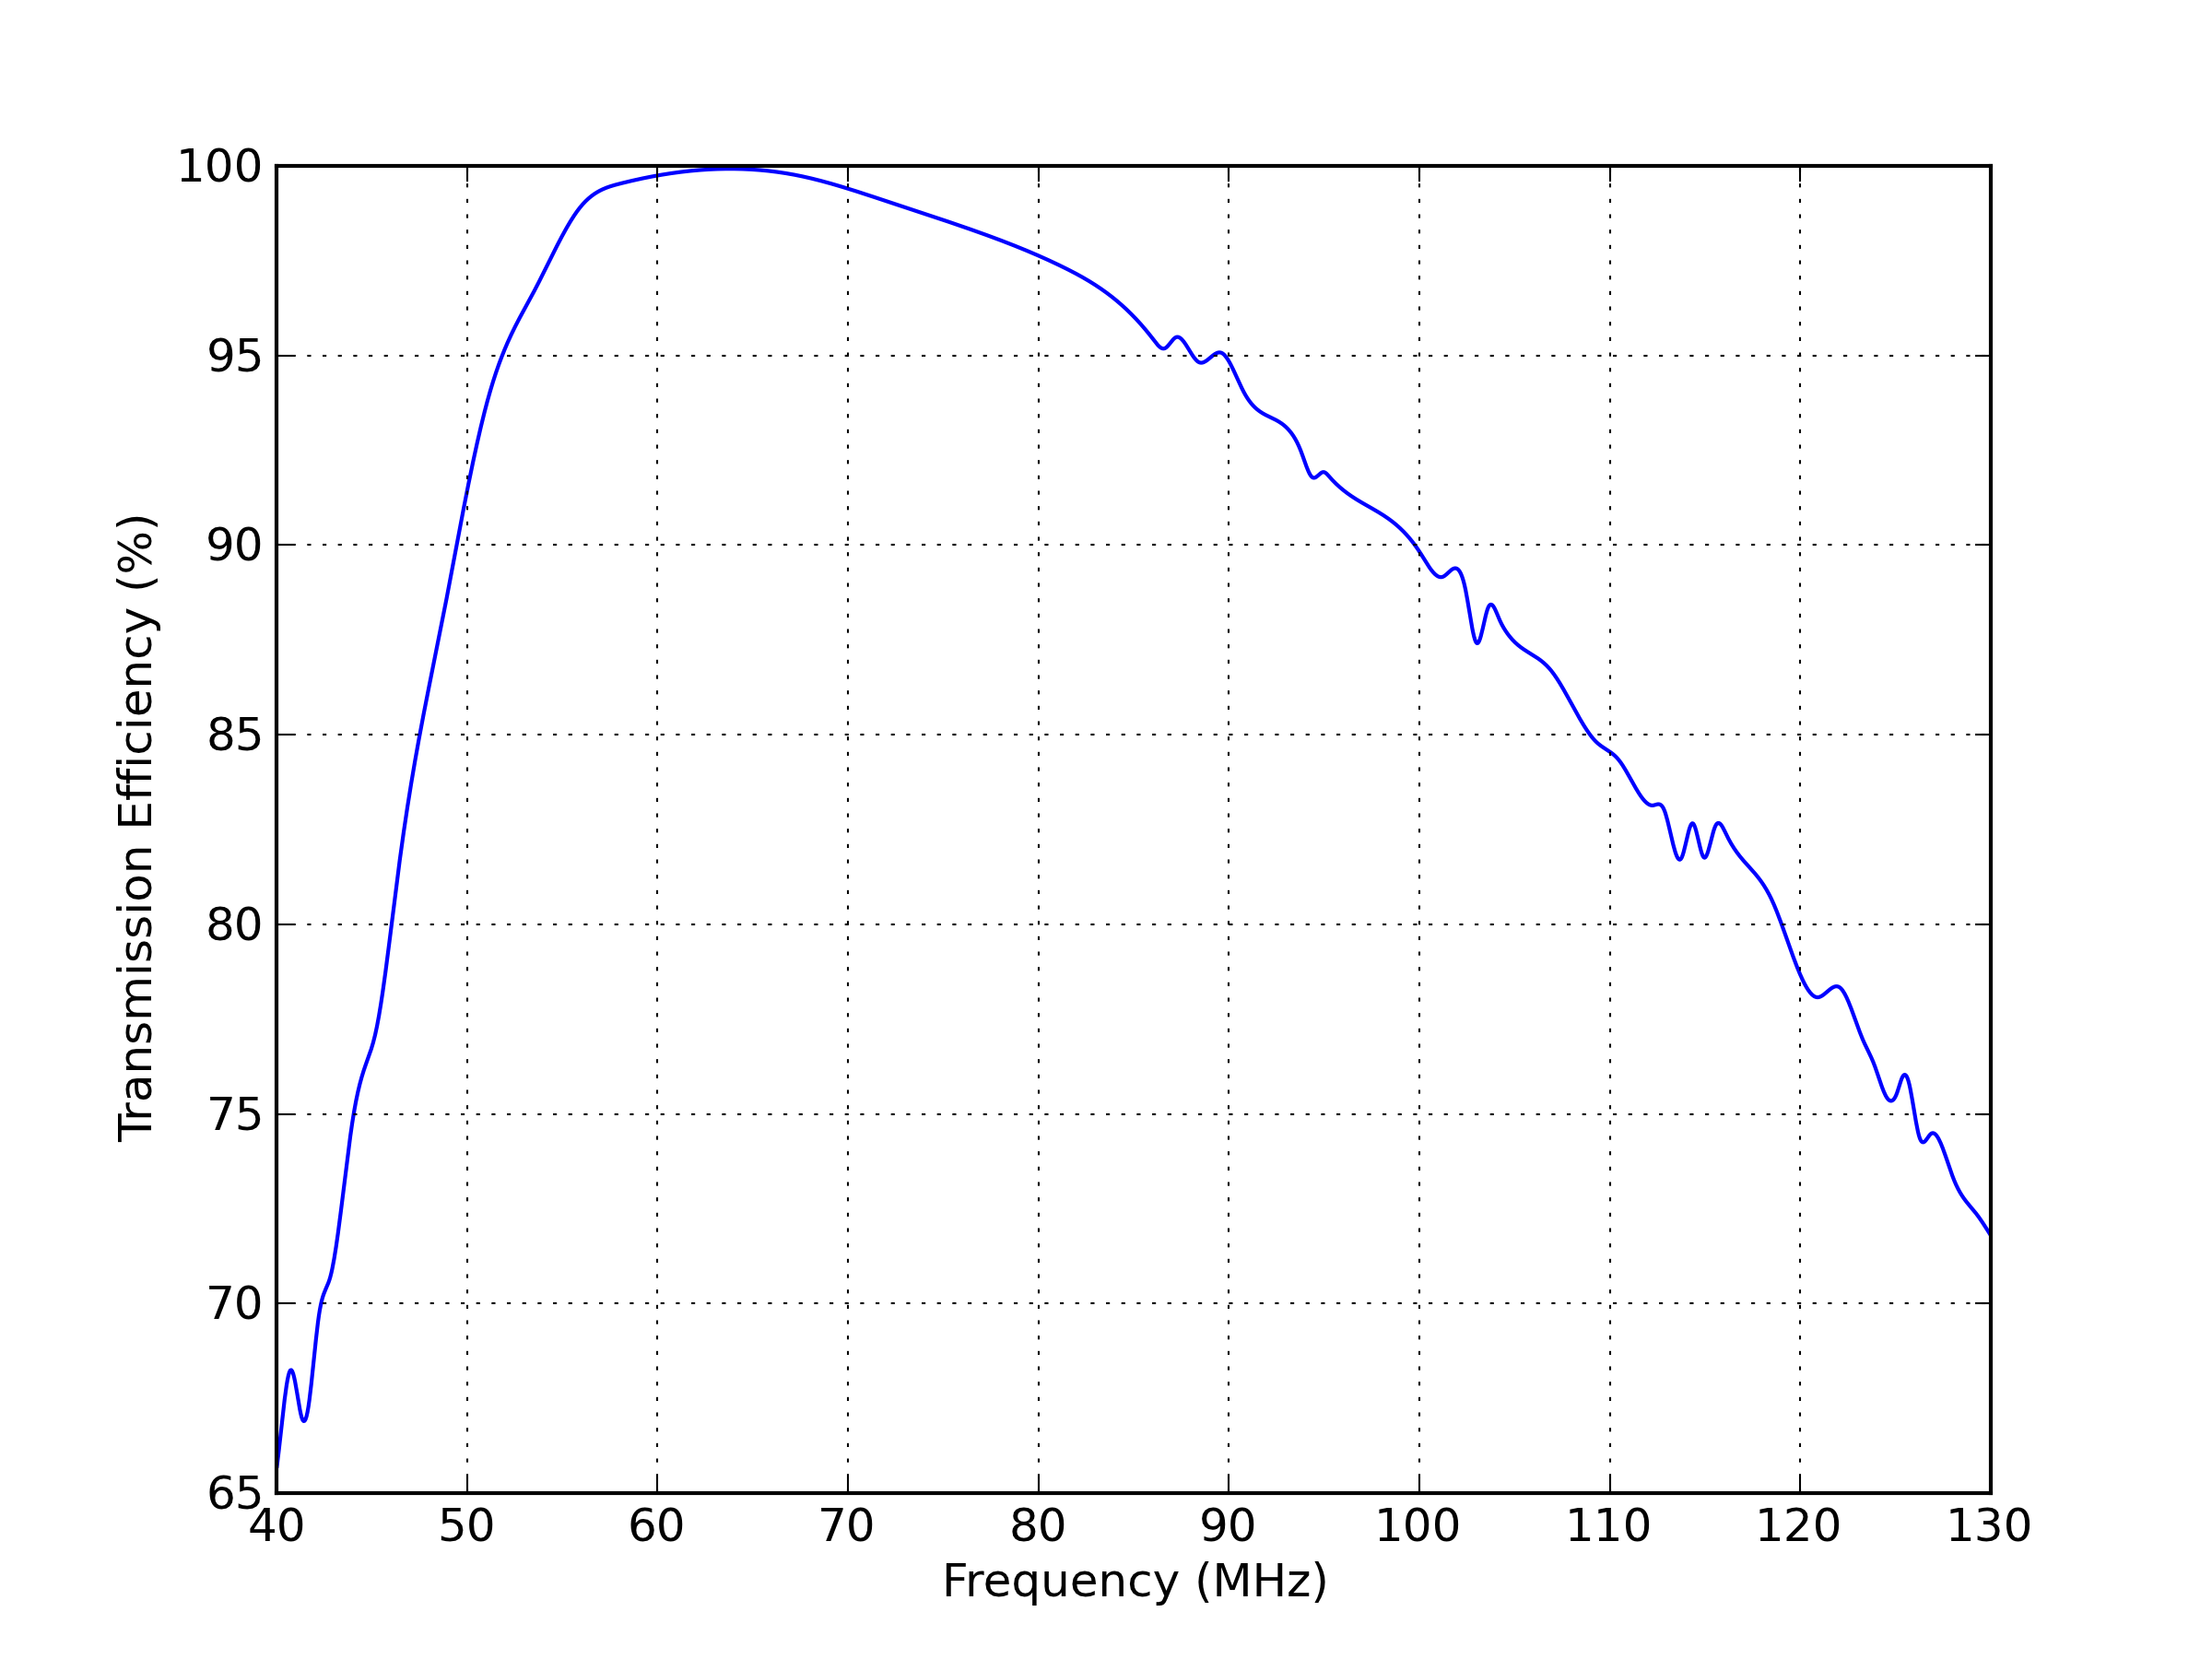
\includegraphics[width=0.9\linewidth]{Data_analysis/figures/old_ant_efficiency.png}
\caption{SCI-HI system transmission efficiency as calculated using S11 measurements of the HIbiscus antenna and first stage amplifier. Here 100 \% efficiency means that all the power from the sky collected by the antenna is seen by the first stage amplifier. }
\label{Fig:eff}
\end{center}
\end{figure}

\subsubsection{Measured Efficiency}

Because the antenna has a non-zero complex phase, the sky signal ($P_{sky}$) measured by the antenna does not all make it into the first stage amplifier. What the amplifier actually sees is ($P_{sky}/\eta$), where the transmission efficiency ($\eta$) was defined in Section \ref{Sec:Amp}. 

For the June 2013 deployment data, the efficiency is shown in Figure \ref{Fig:eff}. With the efficiency, our antenna power equation (\ref{Eq:T_ant}) can be re-written as:

\begin{equation}
P_{Ant}(\nu) = \frac{P_{sky}}{\eta} + P_{short} +P_{thermal}
\end{equation}


\subsection{Milky Way Galaxy (GSM) Modeling} \label{Sec:model}

One of the big challenges of calibration in radio astronomy is figuring out what to use as a known temperature source. For the SCI-HI experiment, the only astronomical source accessible given our $\sim 55 ^\circ$ antenna beam is radio signals from the Milky Way Galaxy. 

\begin{figure}[htb]
\begin{center}
\includegraphics[width=0.9\linewidth]{Data_analysis/figures/beam.pdf}
\caption{Simulated HIbiscus antenna beam on the sky in RA, DEC coordinates at Isla Guadalupe's latitude. Each map corresponds to a different LST at 70 MHz. }
\label{Fig:HIbiscus_beam}
\end{center}
\end{figure}

\subsubsection{HIbiscus Beam Coverage}

Once the SCI-HI system has been set up on-site at a particular location, the Earth rotates as the antenna constantly points towards the zenith. Due to this rotation, the beam of the Hibiscus antenna looks at different parts of the sky at different times of day. 

The exact beam coverage can be calculated using the simulated HIbiscus beam and the site latitude, shown in Figure \ref{Fig:HIbiscus_beam}.  It is important to note that here we use Local Sidereal Time (LST), not Coordinated Universal Time (UTC), because we care about the motion of the Milky Way Galaxy rather than the sun.  

\begin{figure}[htb]
\begin{center}
\includegraphics[width=0.9\linewidth]{Data_analysis/figures/gsm_fig.pdf}
\caption{Sky temperature calculated using the GSM model from de Oliveira-Costa et al \cite{GSM_model} at 70 MHz. The temperature map is in units of $log_{10} Kelvin$, while the map coordinates are in RA, DEC. }
\label{Fig:GSM_model}
\end{center}
\end{figure}

\subsubsection{GSM Model}\label{Sec:GSM}

The main signal from the sky at 40-130 MHz is the Milky Way Galaxy, which has temperatures of over $1000$ Kelvin for most of the SCI-HI frequency band. However, most of the Milky Way Galaxy signal comes from the plane of the galaxy, which moves from horizon to zenith to horizon due to Earth's rotation. This motion causes the galactic plane to drift in and out of the HIbiscus beam over time. 

The Galactic Global Sky Model (GSM) is the current best model for the sky, including the Milky Way Galaxy, at these frequencies. It is a model created by interpolating data from many different publically available radio surveys with a frequency range of $10 MHz - 100 GHz$. The model and software \cite{GSM_model}, can be used to make maps in our frequency band. One such map is shown in Figure \ref{Fig:GSM_model}, displayed using equatorial coordinates (right ascension, RA, and declination, DEC) to match the beam maps. 

\begin{figure}[htb]
\begin{center}
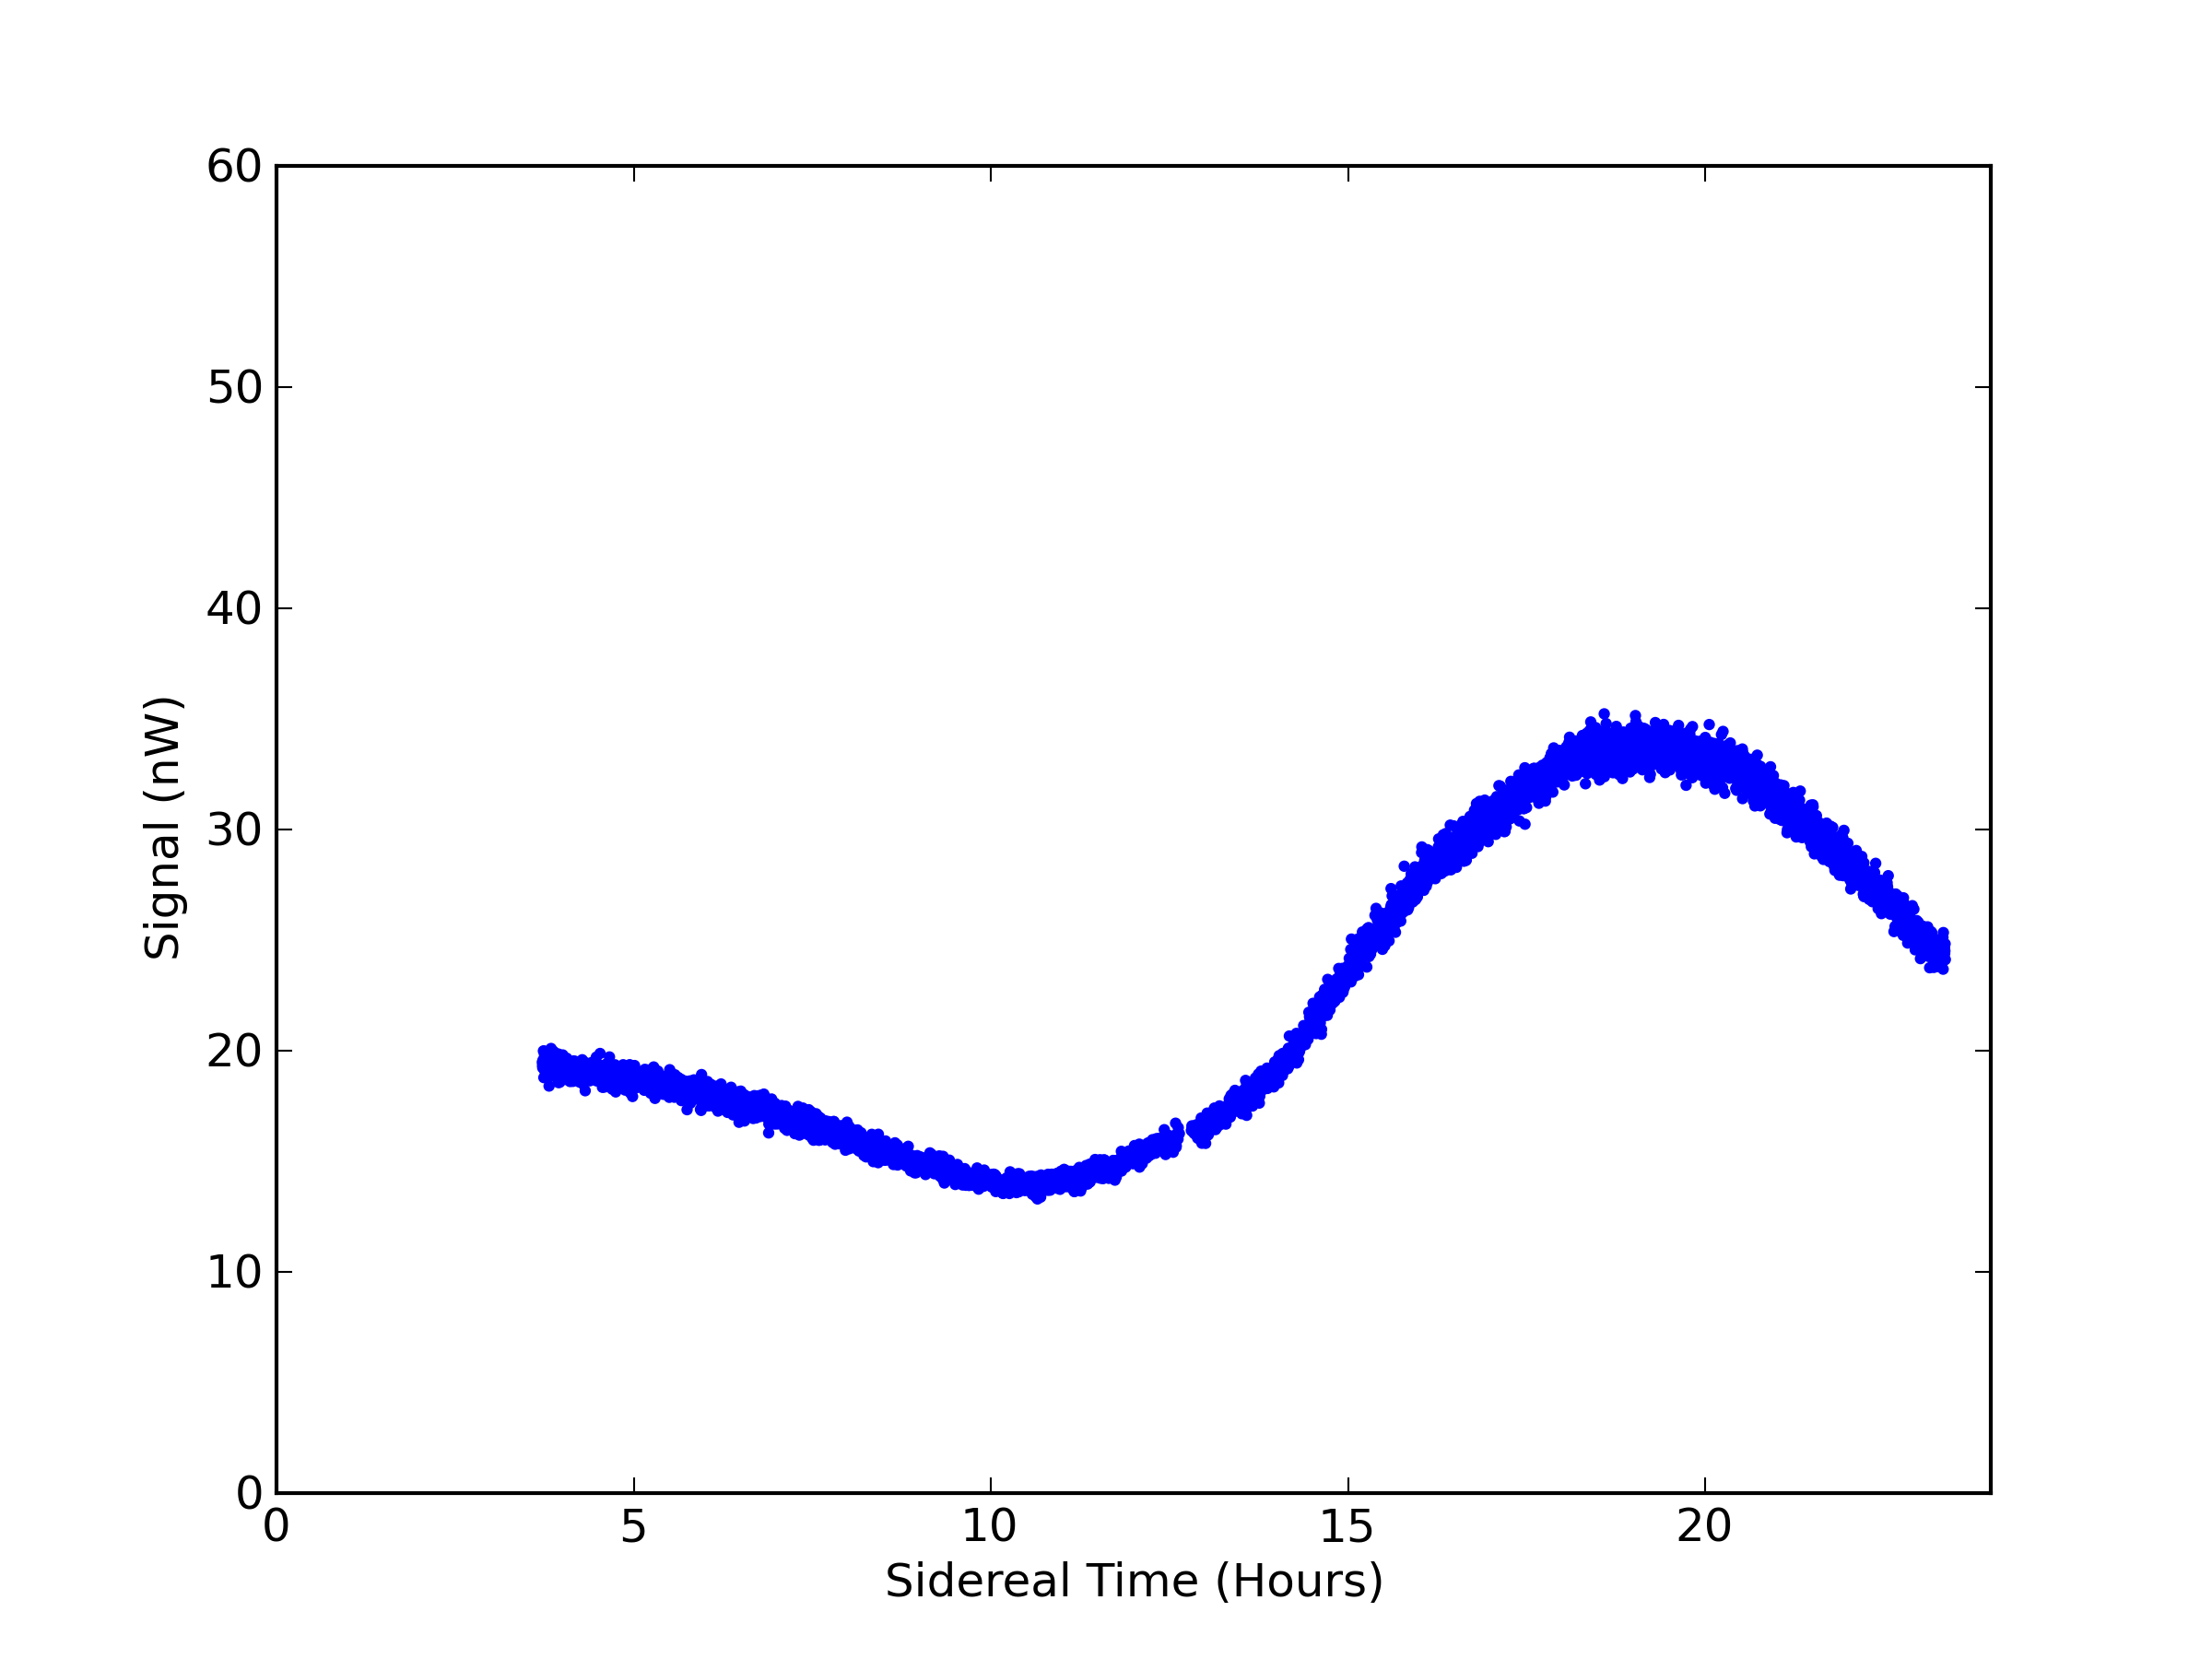
\includegraphics[width=0.9\linewidth]{Data_analysis/figures/June_06_time_series_uncal_70mhz.png}
\caption{Single day plot of uncalibrated data collected with the antenna on June 6th, 2013 at 70 MHz.}
\label{Fig:raw_time_series}
\end{center}
\end{figure}

\subsubsection{Expected Sky Signal}

Using the combination of the GSM model and the simulated HIbiscus antenna beam, the beam-averaged sky temperature can be calculated using the following equation: 

\begin{equation}
T_{GSM} (\nu,t) = \frac{ \int d \Omega GSM (\theta, \phi, \nu) \mathcal{B} (\theta - \theta_0(t), \phi - \phi_0(t),\nu)}{\int d\Omega \mathcal{B} (\theta -\theta_0(t), \phi - \phi_0(t), \nu)}
\end{equation}

Where $GSM (\theta, \phi, \nu)$ is the model data and $\mathcal{B} (\theta - \theta_0(t), \phi - \phi_0(t),\nu)$ is the simulated beam, with ($\theta_0 (t),\phi_0 (t)$) being the beam center. 

This signal is expected to reach a maximum when the Galactic plane is at zenith, and be at a minimum when the Galactic plane is along the horizon. Figure \ref{Fig:raw_time_series} shows that the antenna signal matches this behavior using a single day of data from June 2013, plotted at 70 MHz. 


\subsection{Calibration Factor Calculation}

Now all of our datasets have units of power (dB), as is discussed in Section \ref{Sec:int}. But we want to know the sky signal in units of temperature (Kelvin). Therefore, we need to convert our signals from power to temperature. This conversion can be written with a simple calibration factor $K(\nu)$ such that:

\begin{equation}
T(\nu,t) = K(\nu)*P(\nu,t)
\end{equation}

Calculating the calibration factor can be done with either the known source datasets or the Milky Way Galaxy model. 

\begin{figure}[htb]
\centering
\begin{minipage}[b]{0.48\textwidth}
\centering
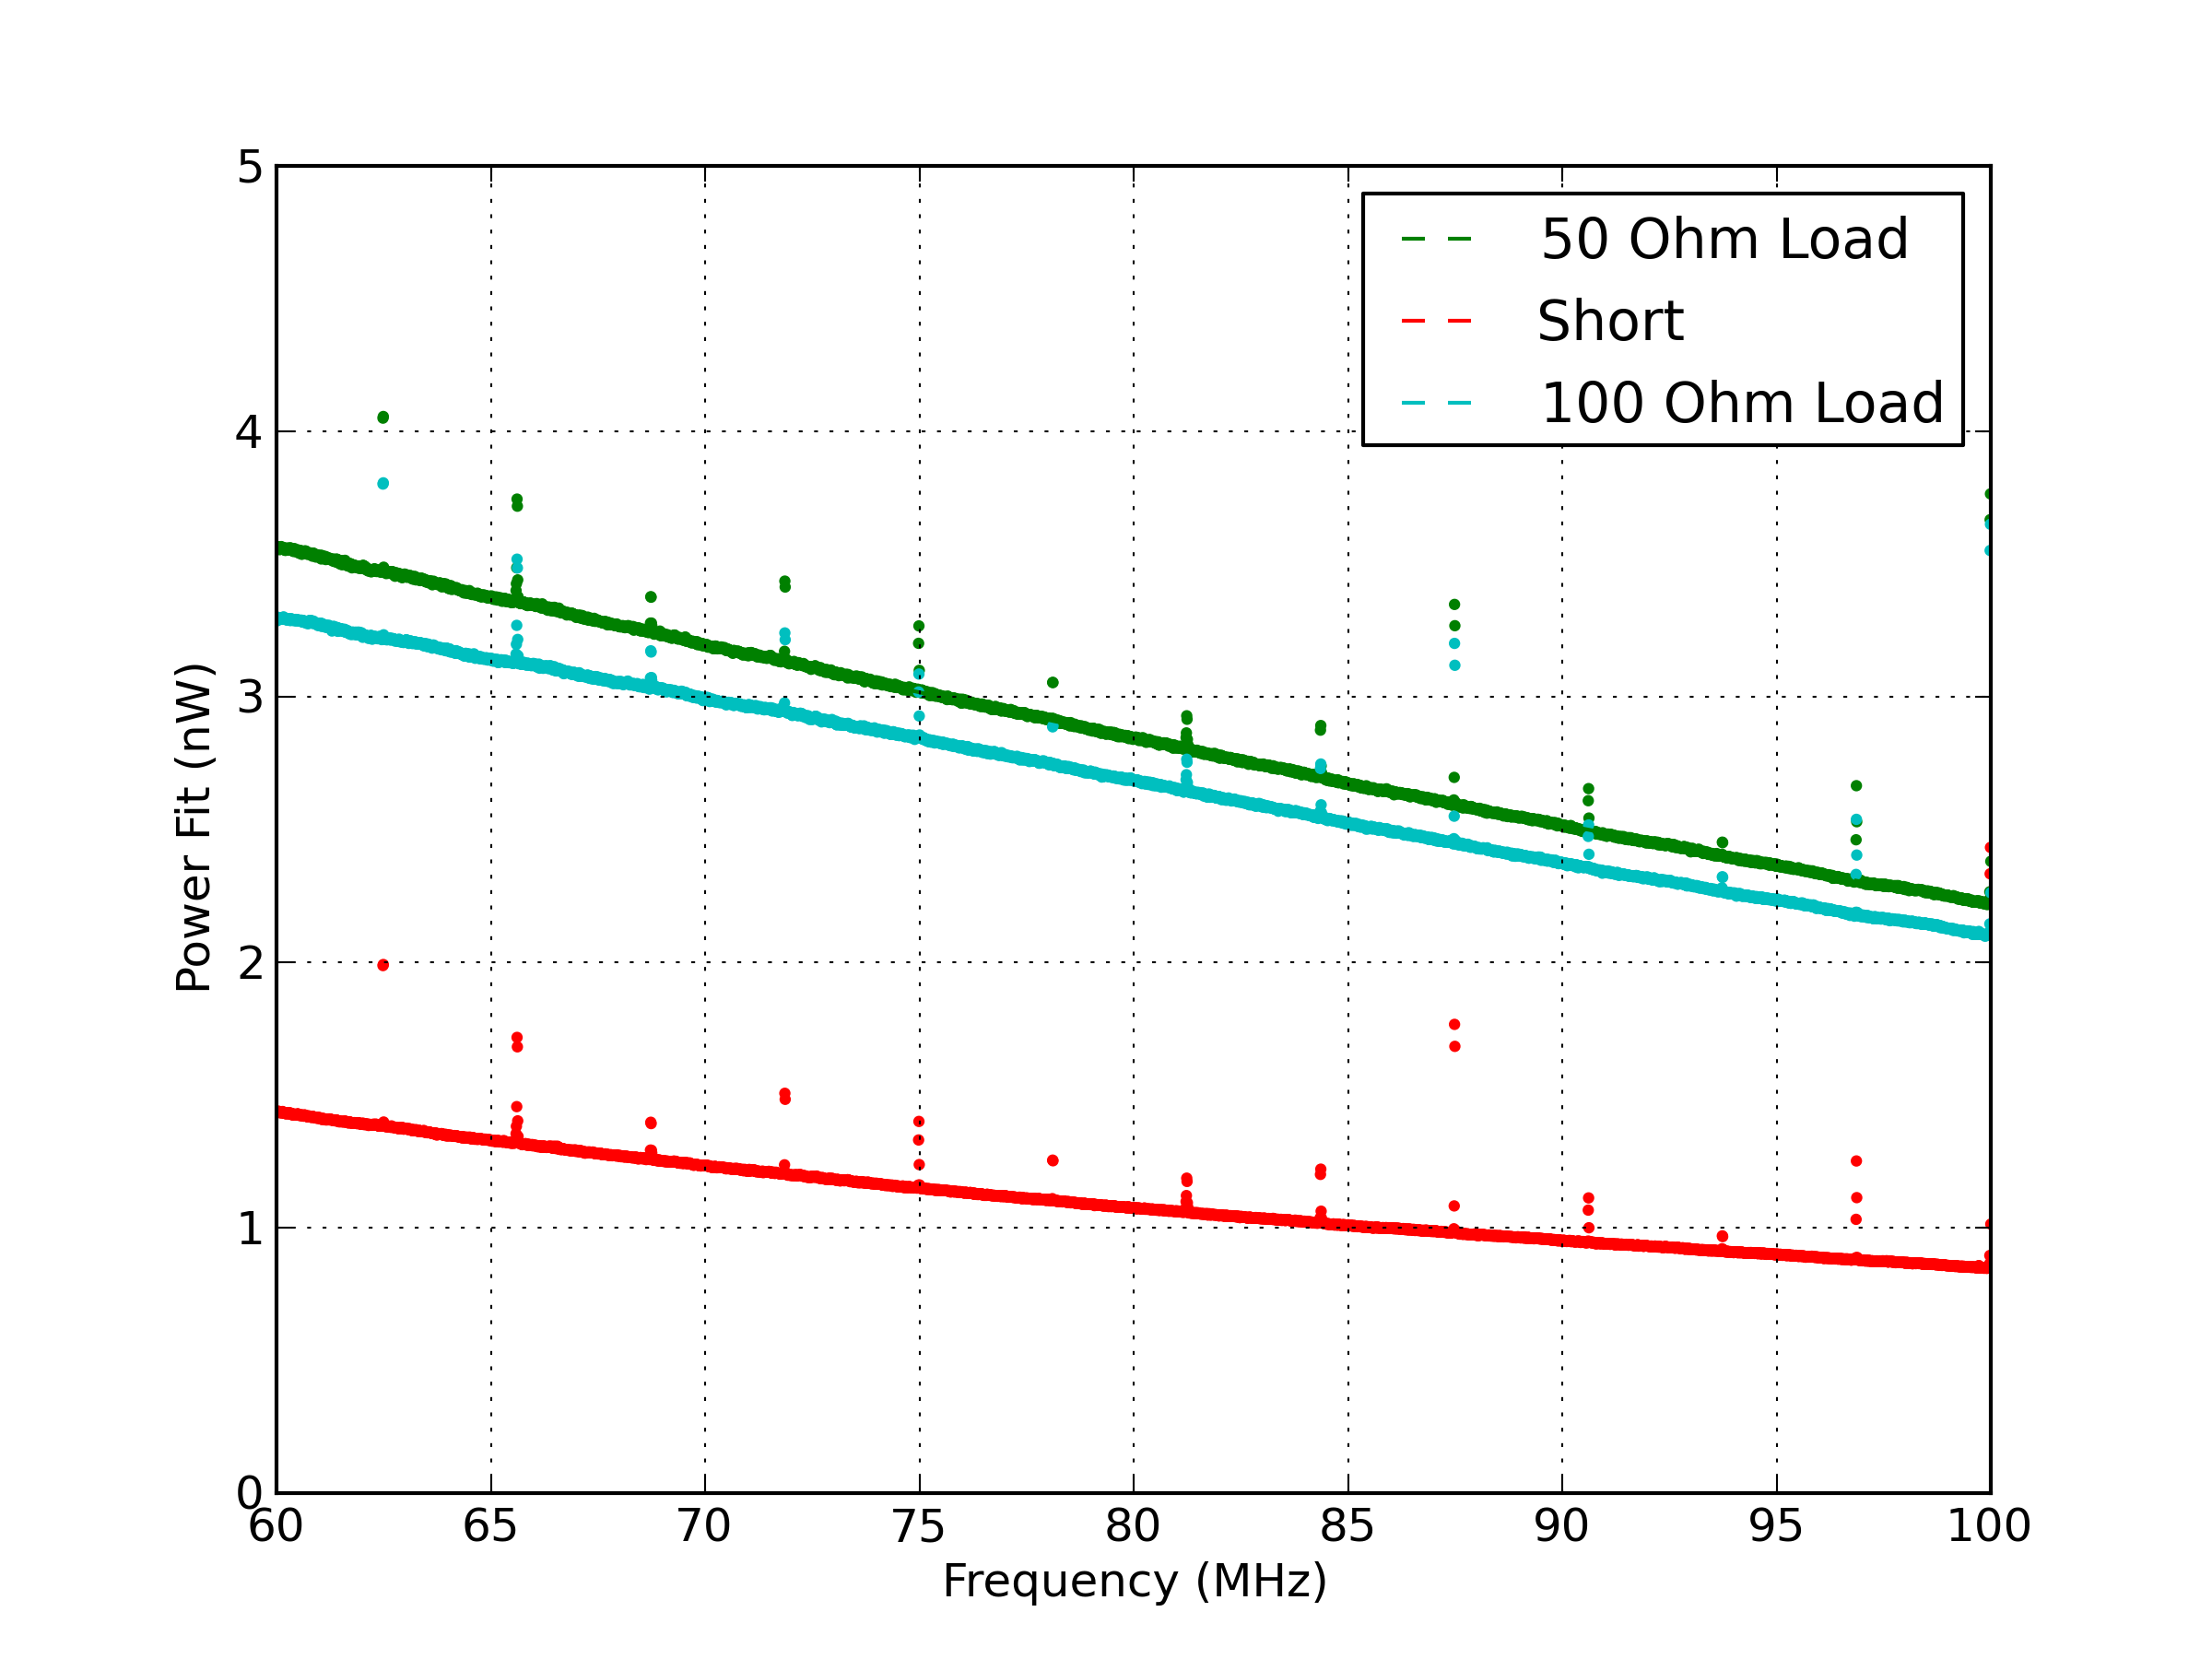
\includegraphics[width=0.95\linewidth]{Data_analysis/figures/June_03_mean_uncal_ref_spectrum_data.png}
\caption{Average of all the calibration datasets for June 3rd, 2013.}
\label{Fig:avg_cal}
\end{minipage}%
\begin{minipage}[b]{0.02\textwidth}
\hspace{1cm}
\end{minipage}%
\begin{minipage}[b]{0.48\textwidth}
\centering
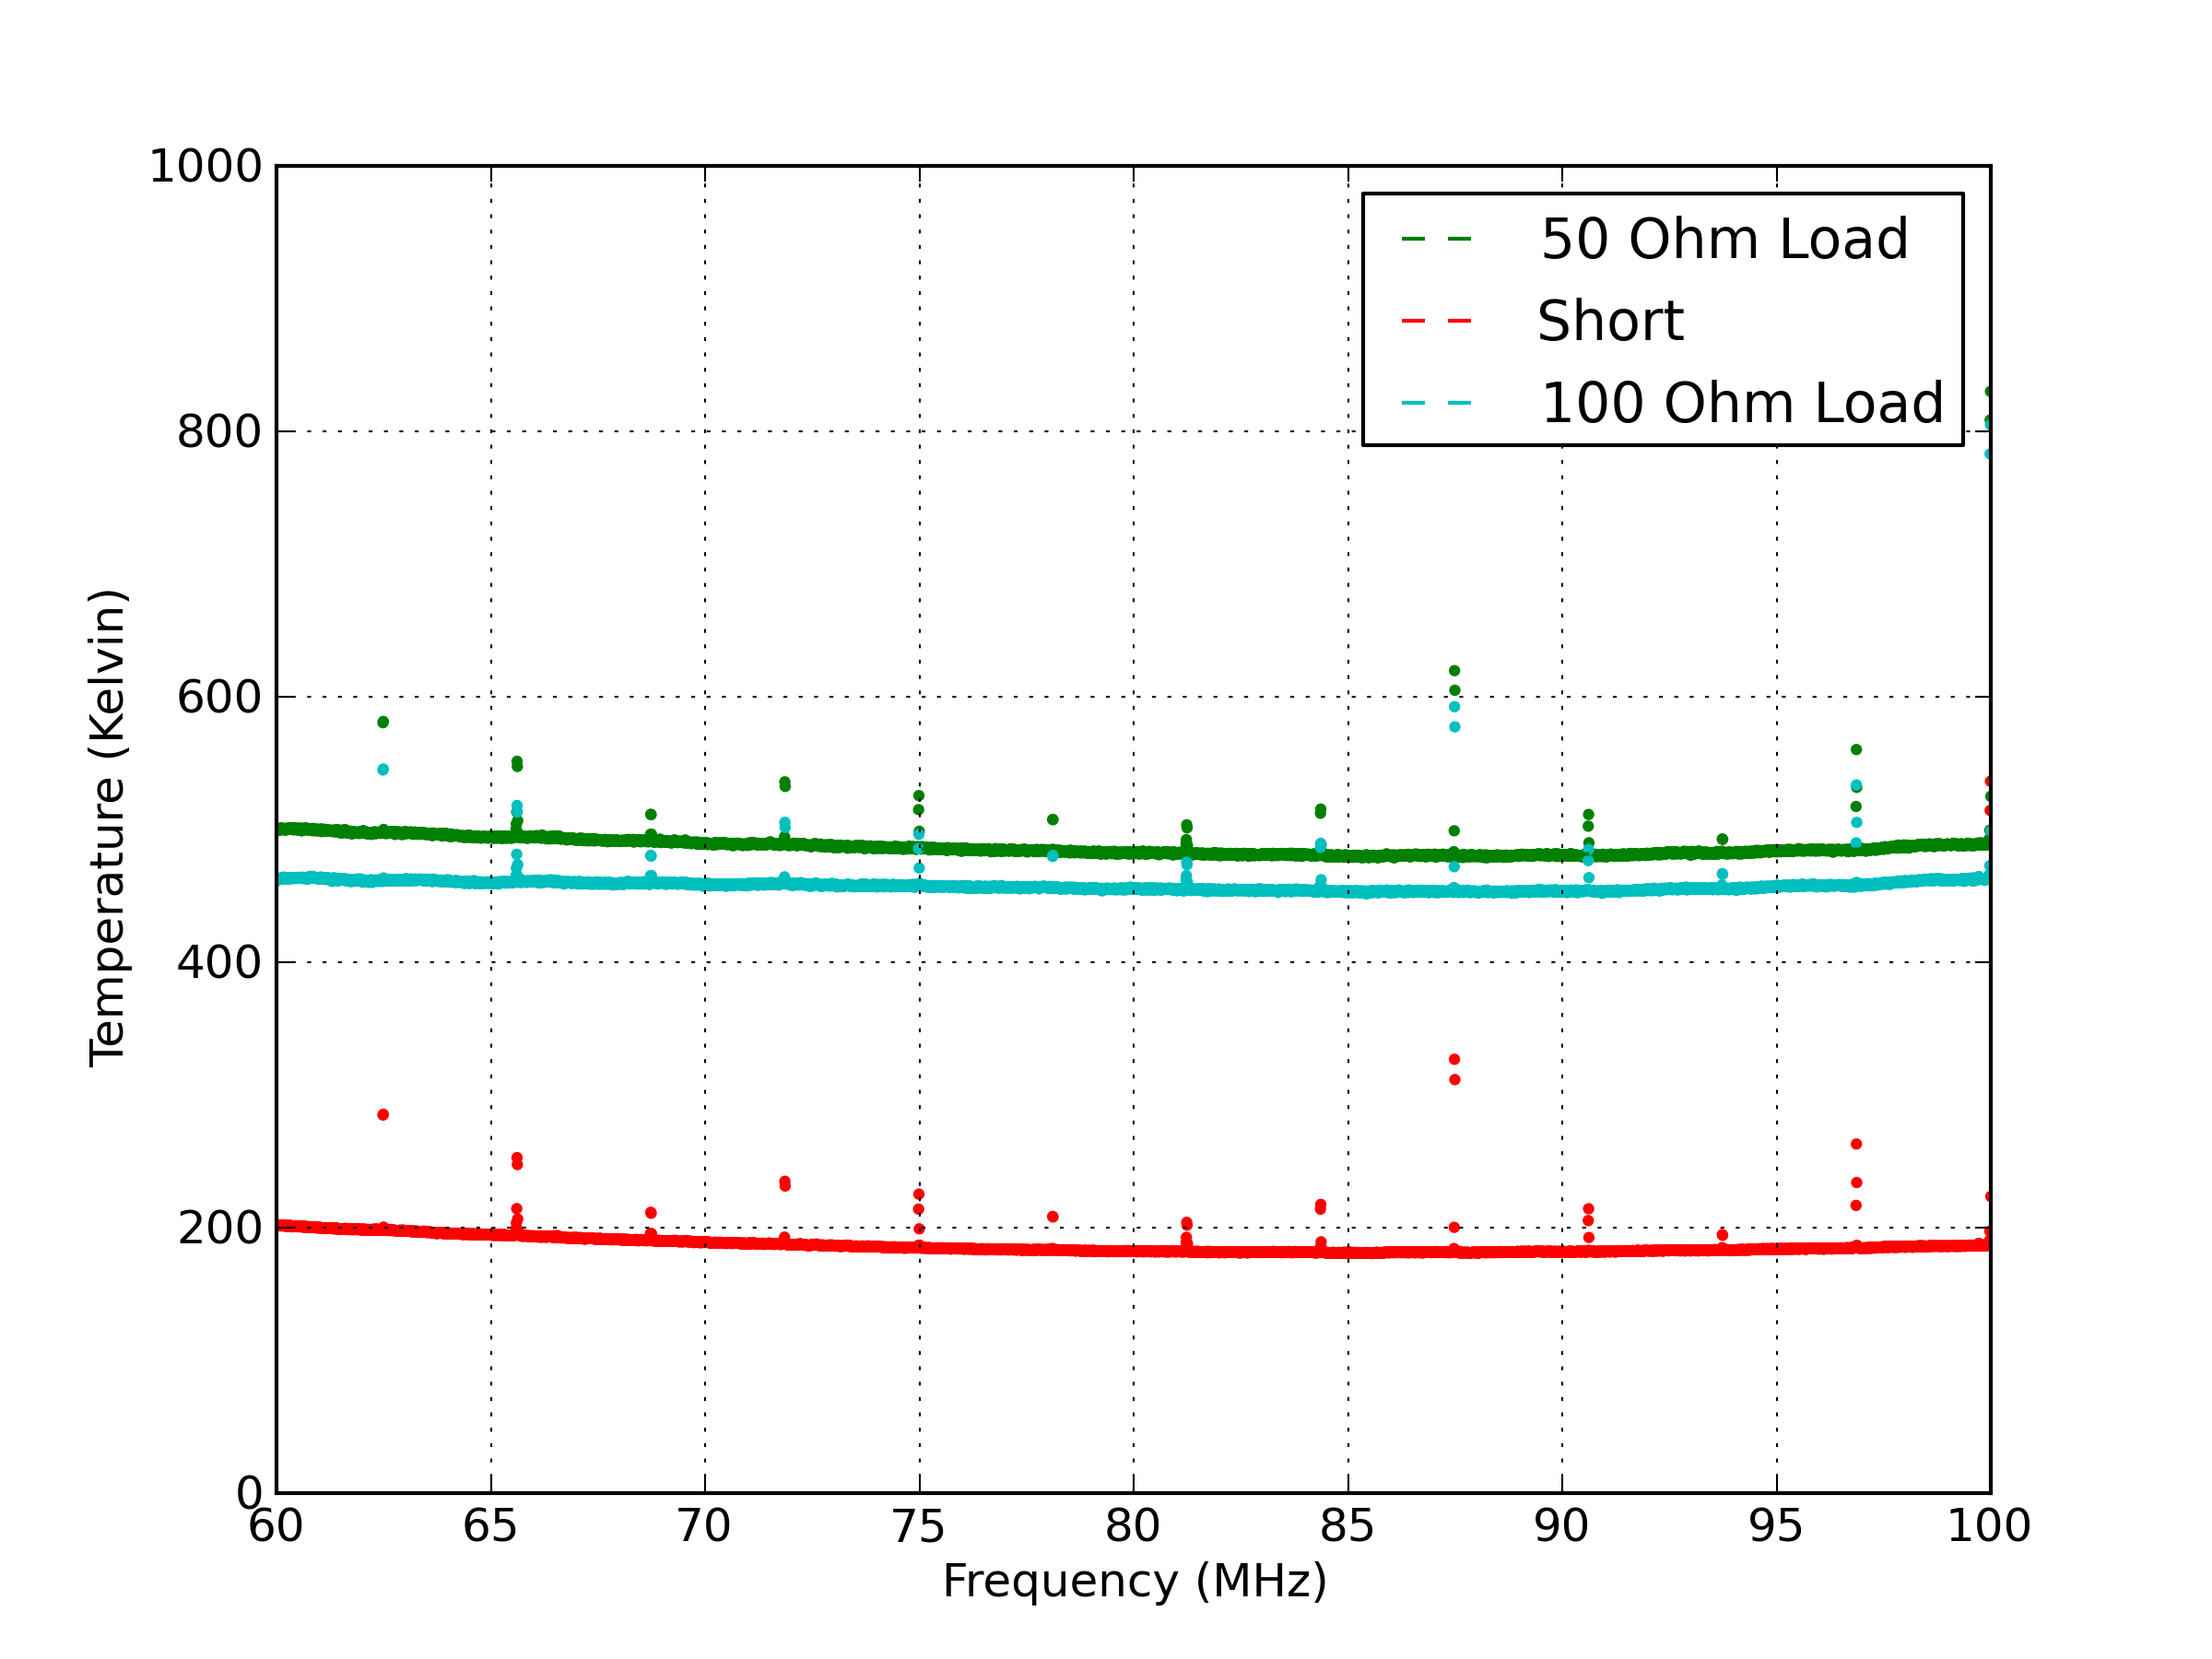
\includegraphics[width=0.95\linewidth]{Data_analysis/figures/June_03_mean_JNCcal_ref_spectrum_data.png}
\caption{Calibrated average of all the calibration datasets for June 3rd, 2013. }
\label{Fig:avg_cal_data}
\end{minipage}
\end{figure}

\subsubsection{Johnson Noise Calibration ($K_{JNC}$)}

Using the Johnson noise datasets, we can determine a calibration factor $K_{JNC}(\nu)$. We start with the following four datasets:

\begin{equation}
T_{short} = K_{JNC}*(P_{short}+P_{thermal})
\end{equation}
\begin{equation}
T_{50 \Omega} = K_{JNC}*P_{50 \Omega} = K_{JNC}*(P_{amb} + P_{Z50} + P_{short}+P_{thermal})
\end{equation}
\begin{equation}
T_{100 \Omega} = K_{JNC}*P_{100 \Omega} = K_{JNC}*(P_{amb} + P_{Z100}+P_{short}+P_{thermal})
\end{equation}
\begin{equation}
T_{NS} = K_{JNC}*P_{NS} = K_{JNC}*(P_{Noise}+P_{amb}+P_{Z50}+P_{short}+P_{thermal})
\end{equation}

By re-arranging the datasets, we get three equations for calculating the calibration factor.

Calibration Equation 1:
\begin{equation}
K_{JNC} = \frac{T_{amb}}{P_{50 \Omega} - P_{short} - P_{Z50}}
\end{equation}

Calibration Equation 2:
\begin{equation}
K_{JNC} = \frac{T_{amb}}{P_{100 \Omega} - P_{short}-P_{Z100}}
\end{equation}

Calibration Equation  3:
\begin{equation}
K_{JNC} = \frac{T_{Noise}}{P_{NS}-P_{50 \Omega}}
\end{equation}

We want to use one (or more) of these equations for our calibration. The noise temperature $T_{Noise}= K_{JNC}*P_{Noise}$ can be measured in the lab prior to installing the noise source, which would allow us to calculate $K_{JNC}$ using Calibration Equation 3. However, if we can't get a high enough quality measurement of $P_{Noise}$ then we will need to use either Calibration Equation 1 or 2. 

In order to use Calibration Equations 1 or 2, we need two things. First, we need to know the ambient temperature $T_{amb} = K_{JNC}*P_{amb}$. Second, we need to know the current noise term $P_{Z50}$ or $P_{Z100}$. The ambient temperature can be measured by installing a temperature sensor near the system, or approximated using a constant approximate ambient temperature. Since Figure \ref{Fig:raw_data} shows $P_{50 \Omega} \approx P_{100 \Omega}$, we know that the current noise term is small. This allows us to run the calibration using Calibration Equation 1, with $P_{Z50} \equiv 0$ and $T_{amb} \equiv 300$K. 

\subsubsection{Thermal Noise Contribution}

Now, for all of these Calibration Equations I've dropped the thermal noise term ($P_{thermal}$). I can do this because thermal noise is random gaussian fluctuations in the signal whose magnitude is defined by the radiometer equation ($P_{thermal} = P_{total}/\sqrt{\Delta \nu \Delta t}$), where $\Delta \nu$ is the frequency resolution of the data in Hz and $\Delta t$ is the integration time in seconds \cite{stutzman1981}. 

Therefore, thermal noise can be lowered by averaging many calibration datasets (increasing $\Delta t$). Figure \ref{Fig:avg_cal} shows the averaged data for one full day. Once we've taken the averages, we can further lower the thermal noise contribution by fitting the averages to a simple polynomial in frequency over a large frequency band, increasing $\Delta \nu$. We used $P = b_0 + b_1 \nu +b_2 \nu^2$ for our fit, with the frequency band of $50 \leq \nu \leq 100$MHz. 

Figure \ref{Fig:avg_cal_data} shows the average of the calibration datasets after Calibration Equation 1 is used to calculate $K_{JNC}$. Note that our assumption that $P_{Z50}=0$ is approximately, but not exactly, correct since $P_{50 \Omega} \neq P_{100 \Omega}$. Figure \ref{Fig:avg_JNCcal_data} shows the calibrated average of one day of antenna data and the reference spectra used for that calibration. 

\begin{figure}[htb]
\centering
\begin{minipage}[b]{0.48\textwidth}
\centering
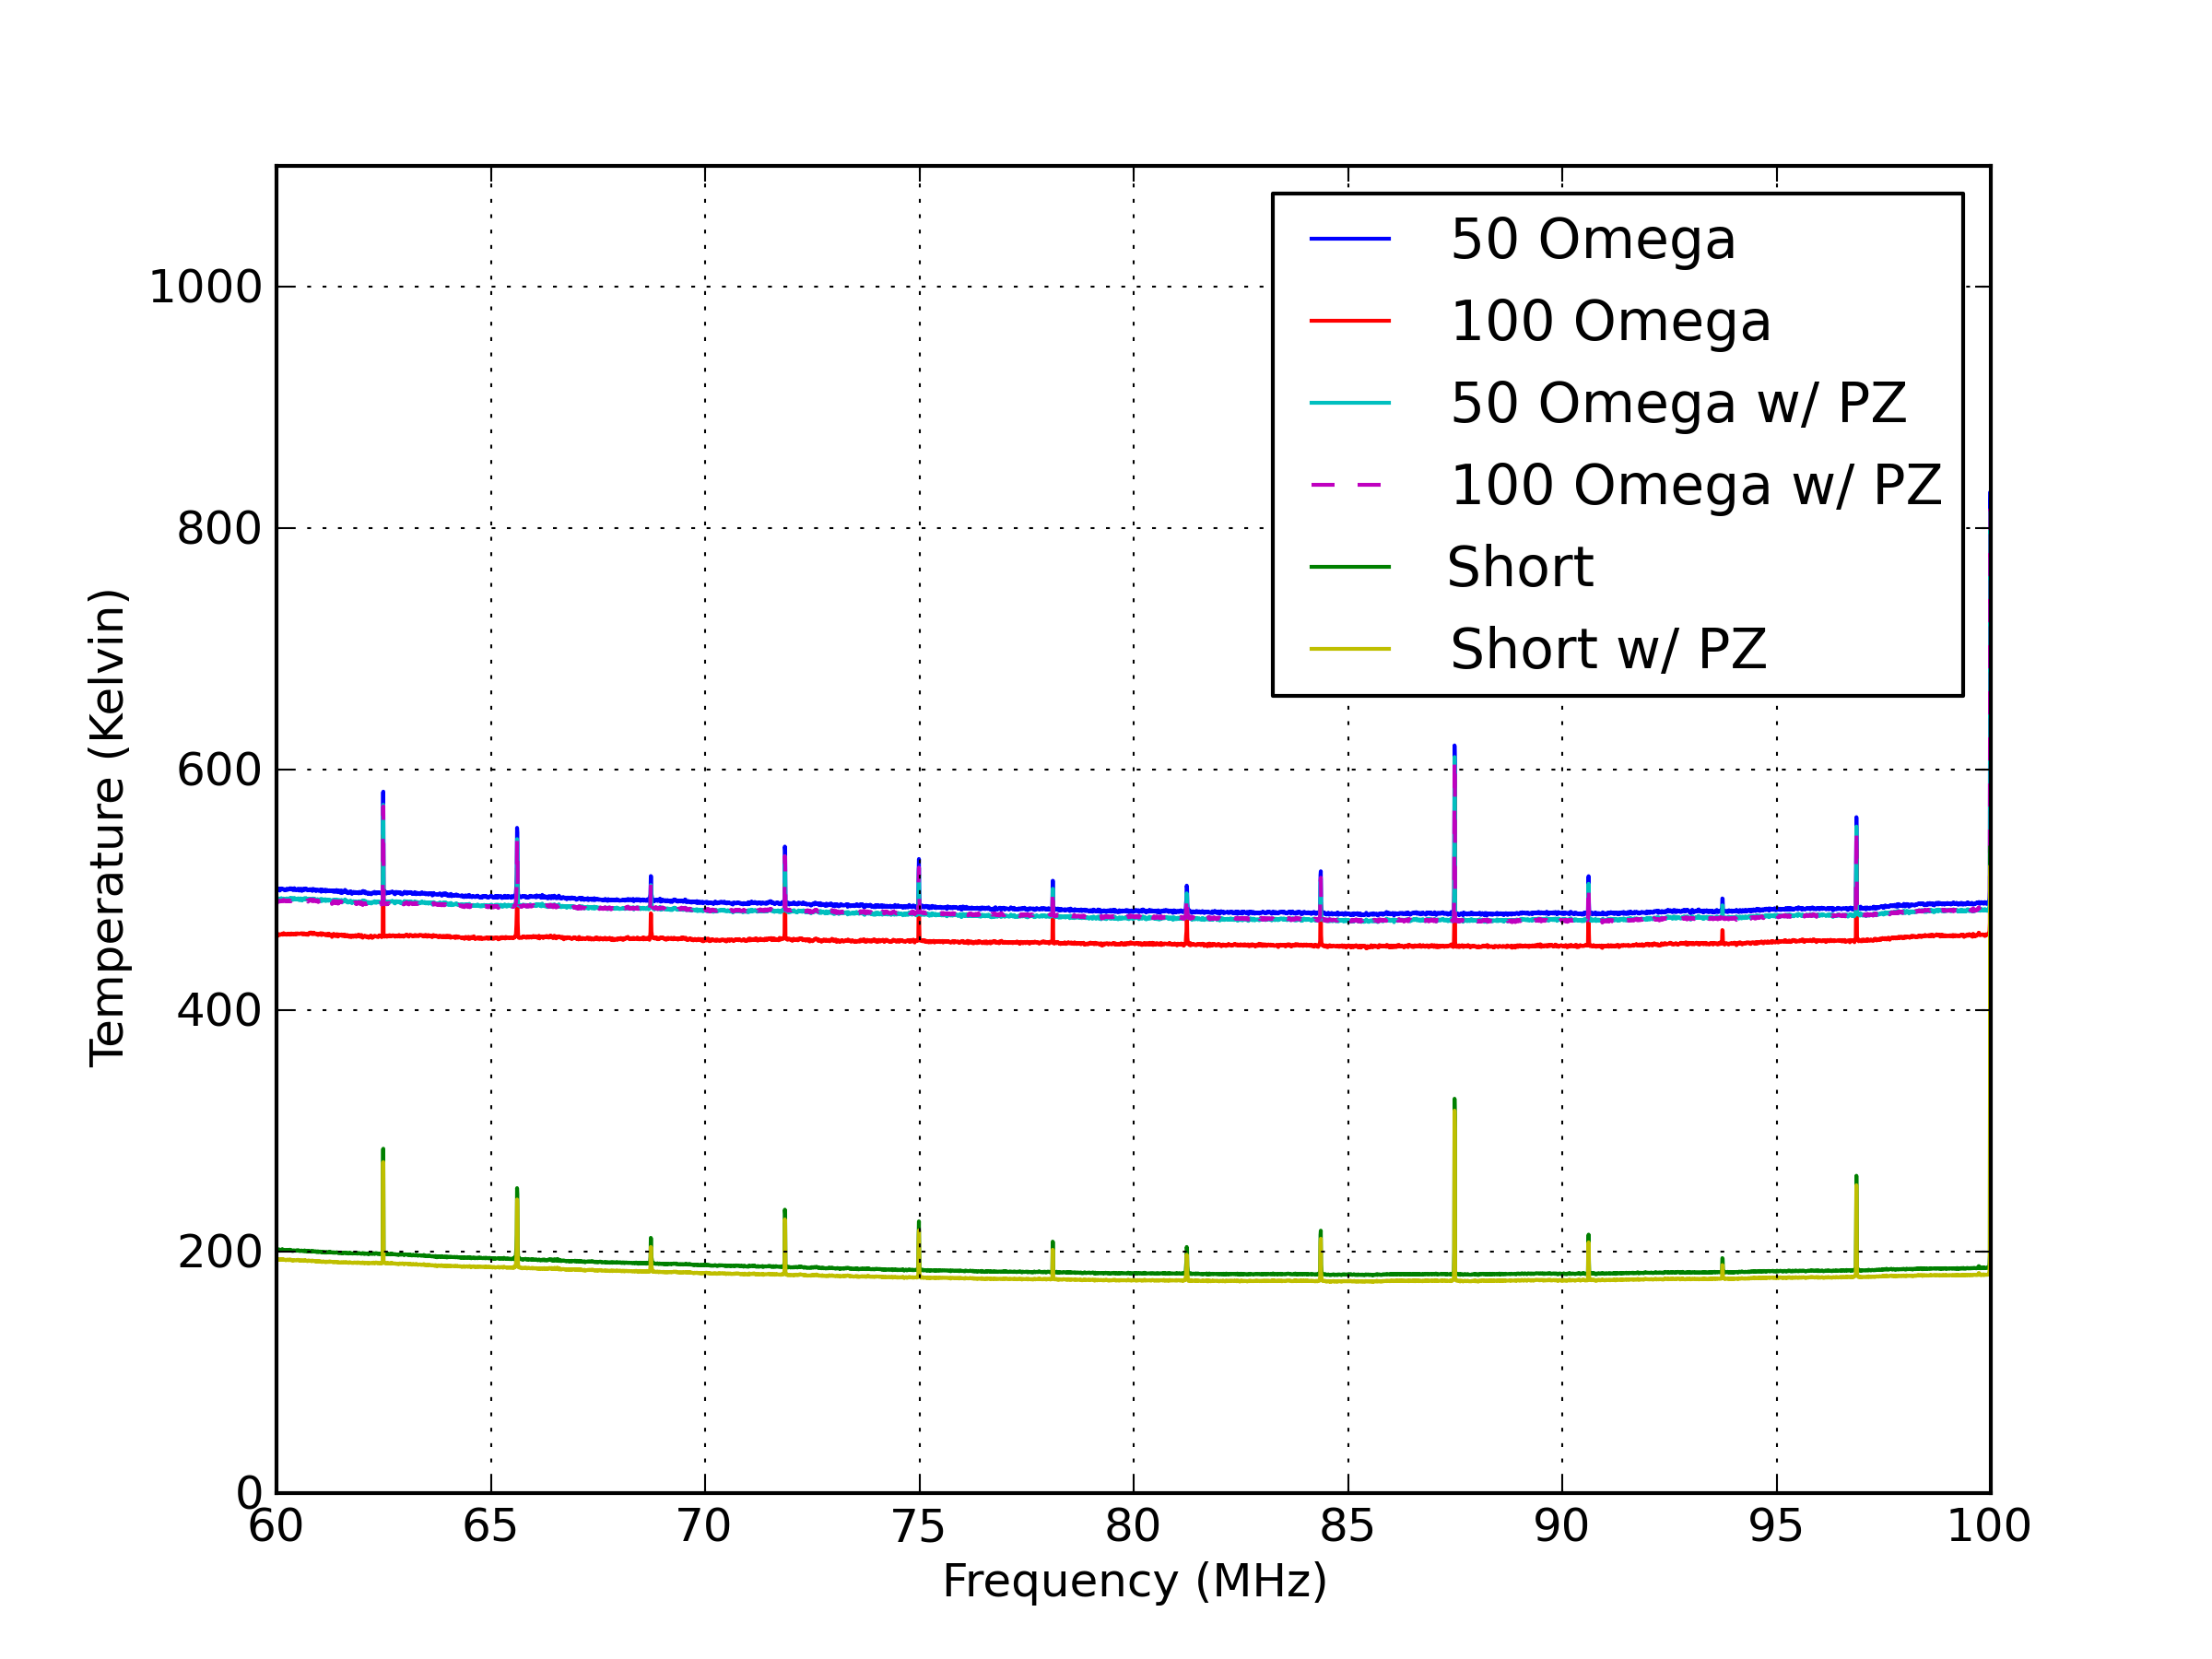
\includegraphics[width=0.95\linewidth]{Data_analysis/figures/June_03_comp_test.png}
\caption{Comparison calibrated averages of all the calibration datasets for June 3rd, 2013 before/after including the current noise contribution to the calibration. }
\label{Fig:avg_cal_comp}
\end{minipage}%
\begin{minipage}[b]{0.02\textwidth}
\hspace{1cm}
\end{minipage}%
\begin{minipage}[b]{0.48\textwidth}
\centering
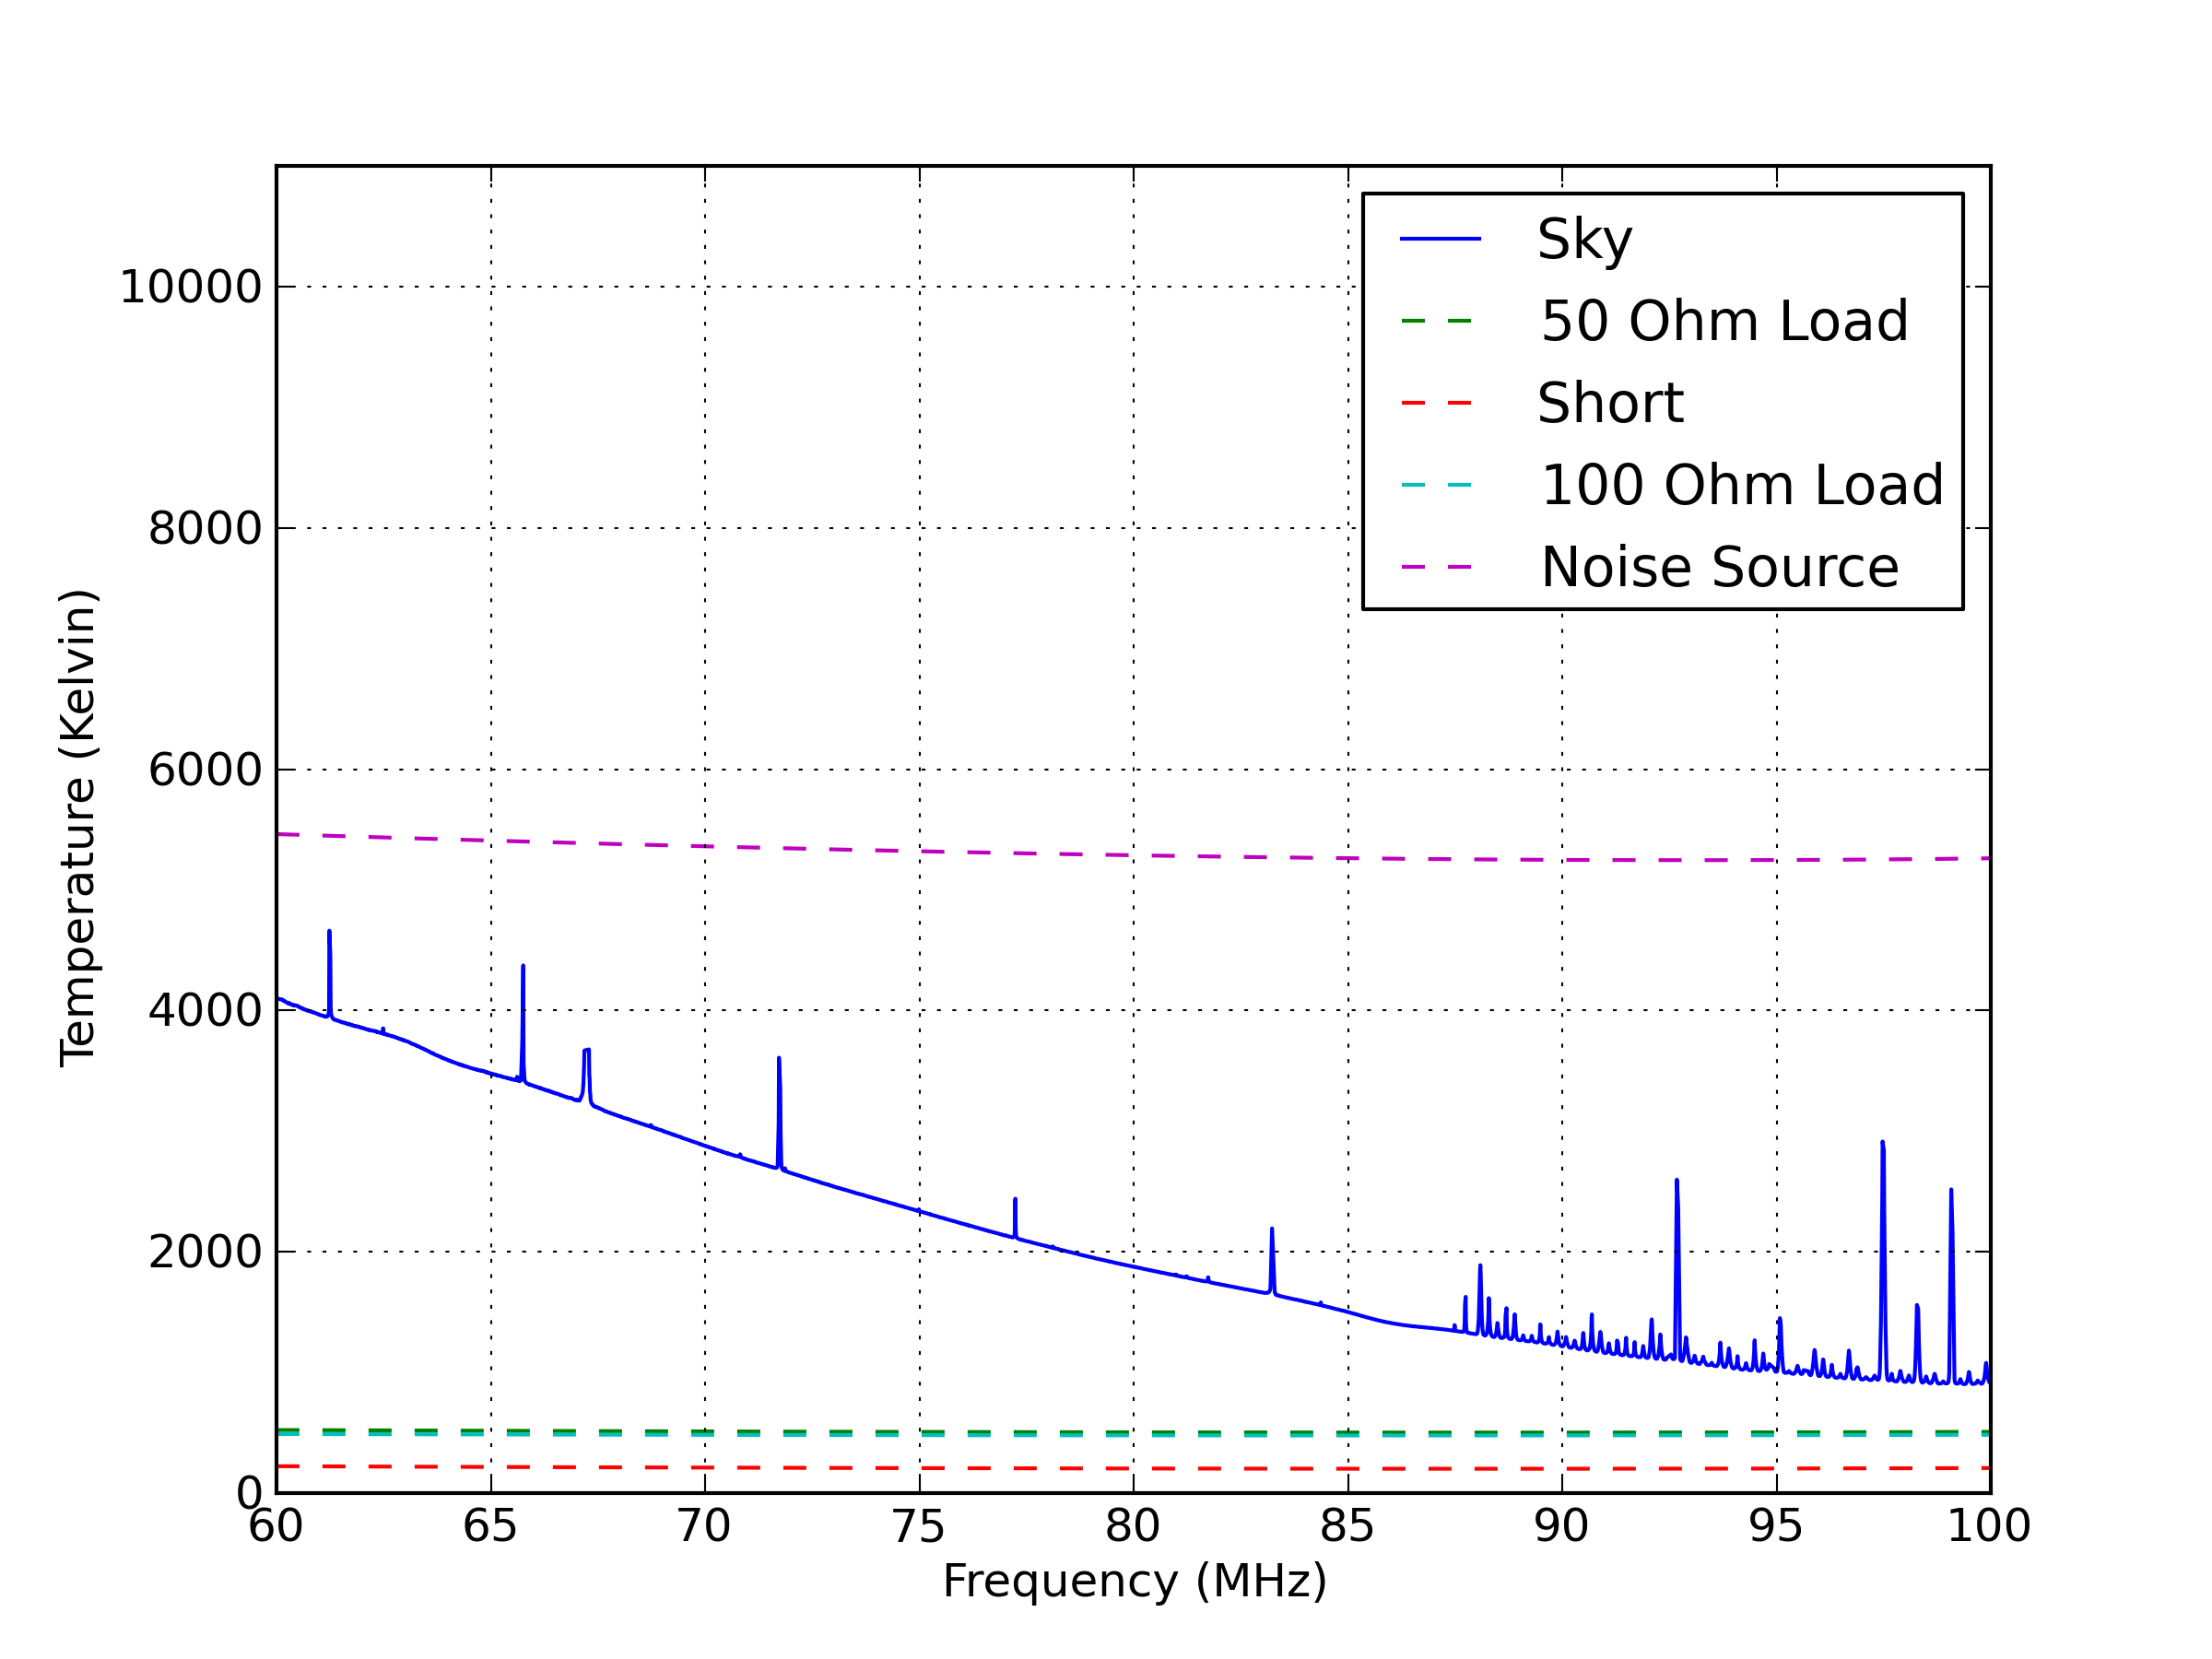
\includegraphics[width=0.95\linewidth]{Data_analysis/figures/June_01_mean_JNCcal_spectrum_full_ref.png}
\caption{JNC Calibrated average of all the data taken on June 1st, 2013; along with the fits for the average calibrated datasets. Data is plotted at high-frequency resolution prior to re-binning. }
\label{Fig:avg_JNCcal_data}
\end{minipage}
\end{figure}

\subsubsection{Current Noise Contribution}

In order to include a non-zero $P_Z$ component in the calibration, we can use the difference between $P_{50 \Omega}$ and $P_{100 \Omega}$. $P \propto |Z|^2 \eta_{Z}$, where $\eta_Z$ is the transmission efficiency if the amplifier is attached to a $50 \Omega$ or $100 \Omega$ terminator. By taking the difference $P_{50 \Omega}-P_{100 \Omega}$, we can calculate a proportionality constant:

\begin{equation}
A = \frac{P_{50 \Omega} - P_{100 \Omega}}{\eta_{50 \Omega} - 4 \eta_{100 \Omega}}
\end{equation}

Using this proportionality constant we get a value for $P_{Z} = A |Z|^2 \eta_{Z}$, which can be plugged into Calibration Equations 1 and 2. We can then calculate the contribution to the system noise from this correction. This is done by comparing $T_{short}$ for the original and modified calibration. The modified calibration gives a lower $T_{short}$ across the entire frequency band of $60 \leq \nu \leq 100$ MHz. This value is lower for all days of data and the difference has an average magnitude of $\Delta T_{short} = 8.359 \pm 1.020$ Kelvin. Figure \ref{Fig:avg_cal_comp} matches Figure \ref{Fig:avg_cal} with the addition of data calibrated with a calculated $P_{Z}$.

\begin{figure}[htb]
\begin{center}
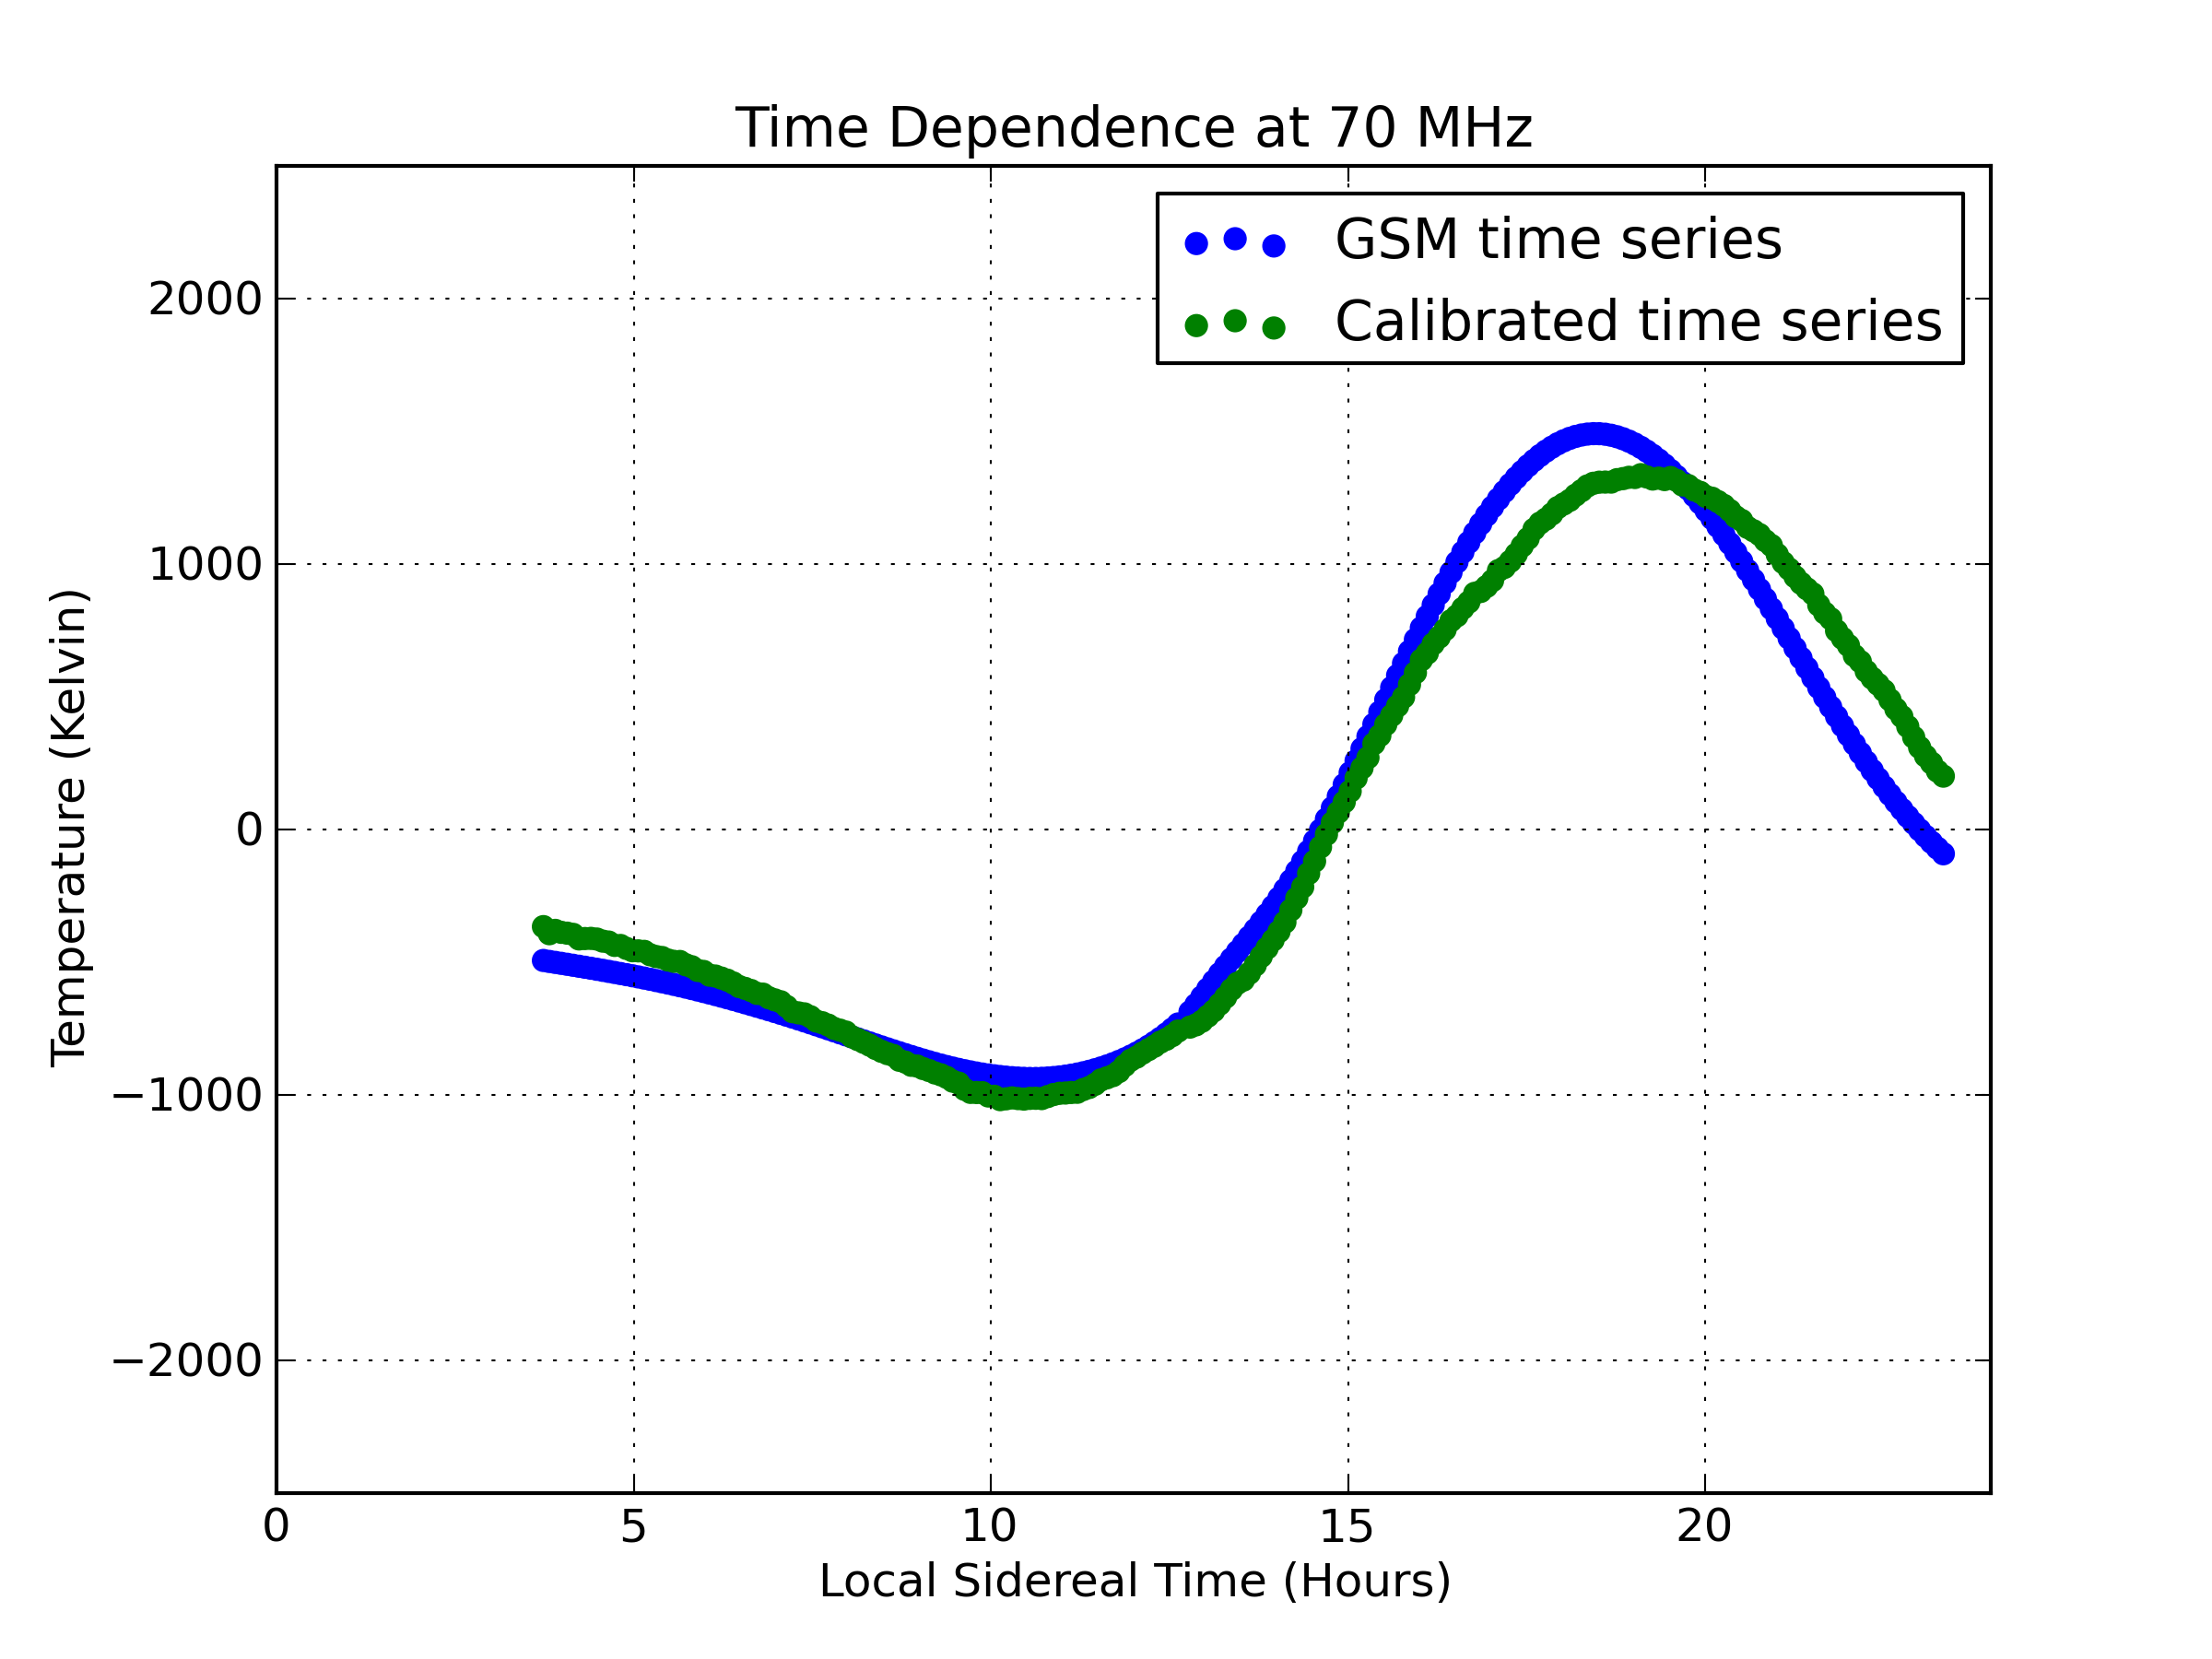
\includegraphics[width=0.95\linewidth]{Data_analysis/figures/June_06_K_dgsm_time_series.png}
\caption{Single day fit of the $K_{\Delta GSM}$ calibration term with data collected on June 6th, 2013 at 70 MHz. }
\label{Fig:Kdgsm}
\end{center}
\end{figure}

\begin{figure}[htb]
\begin{center}
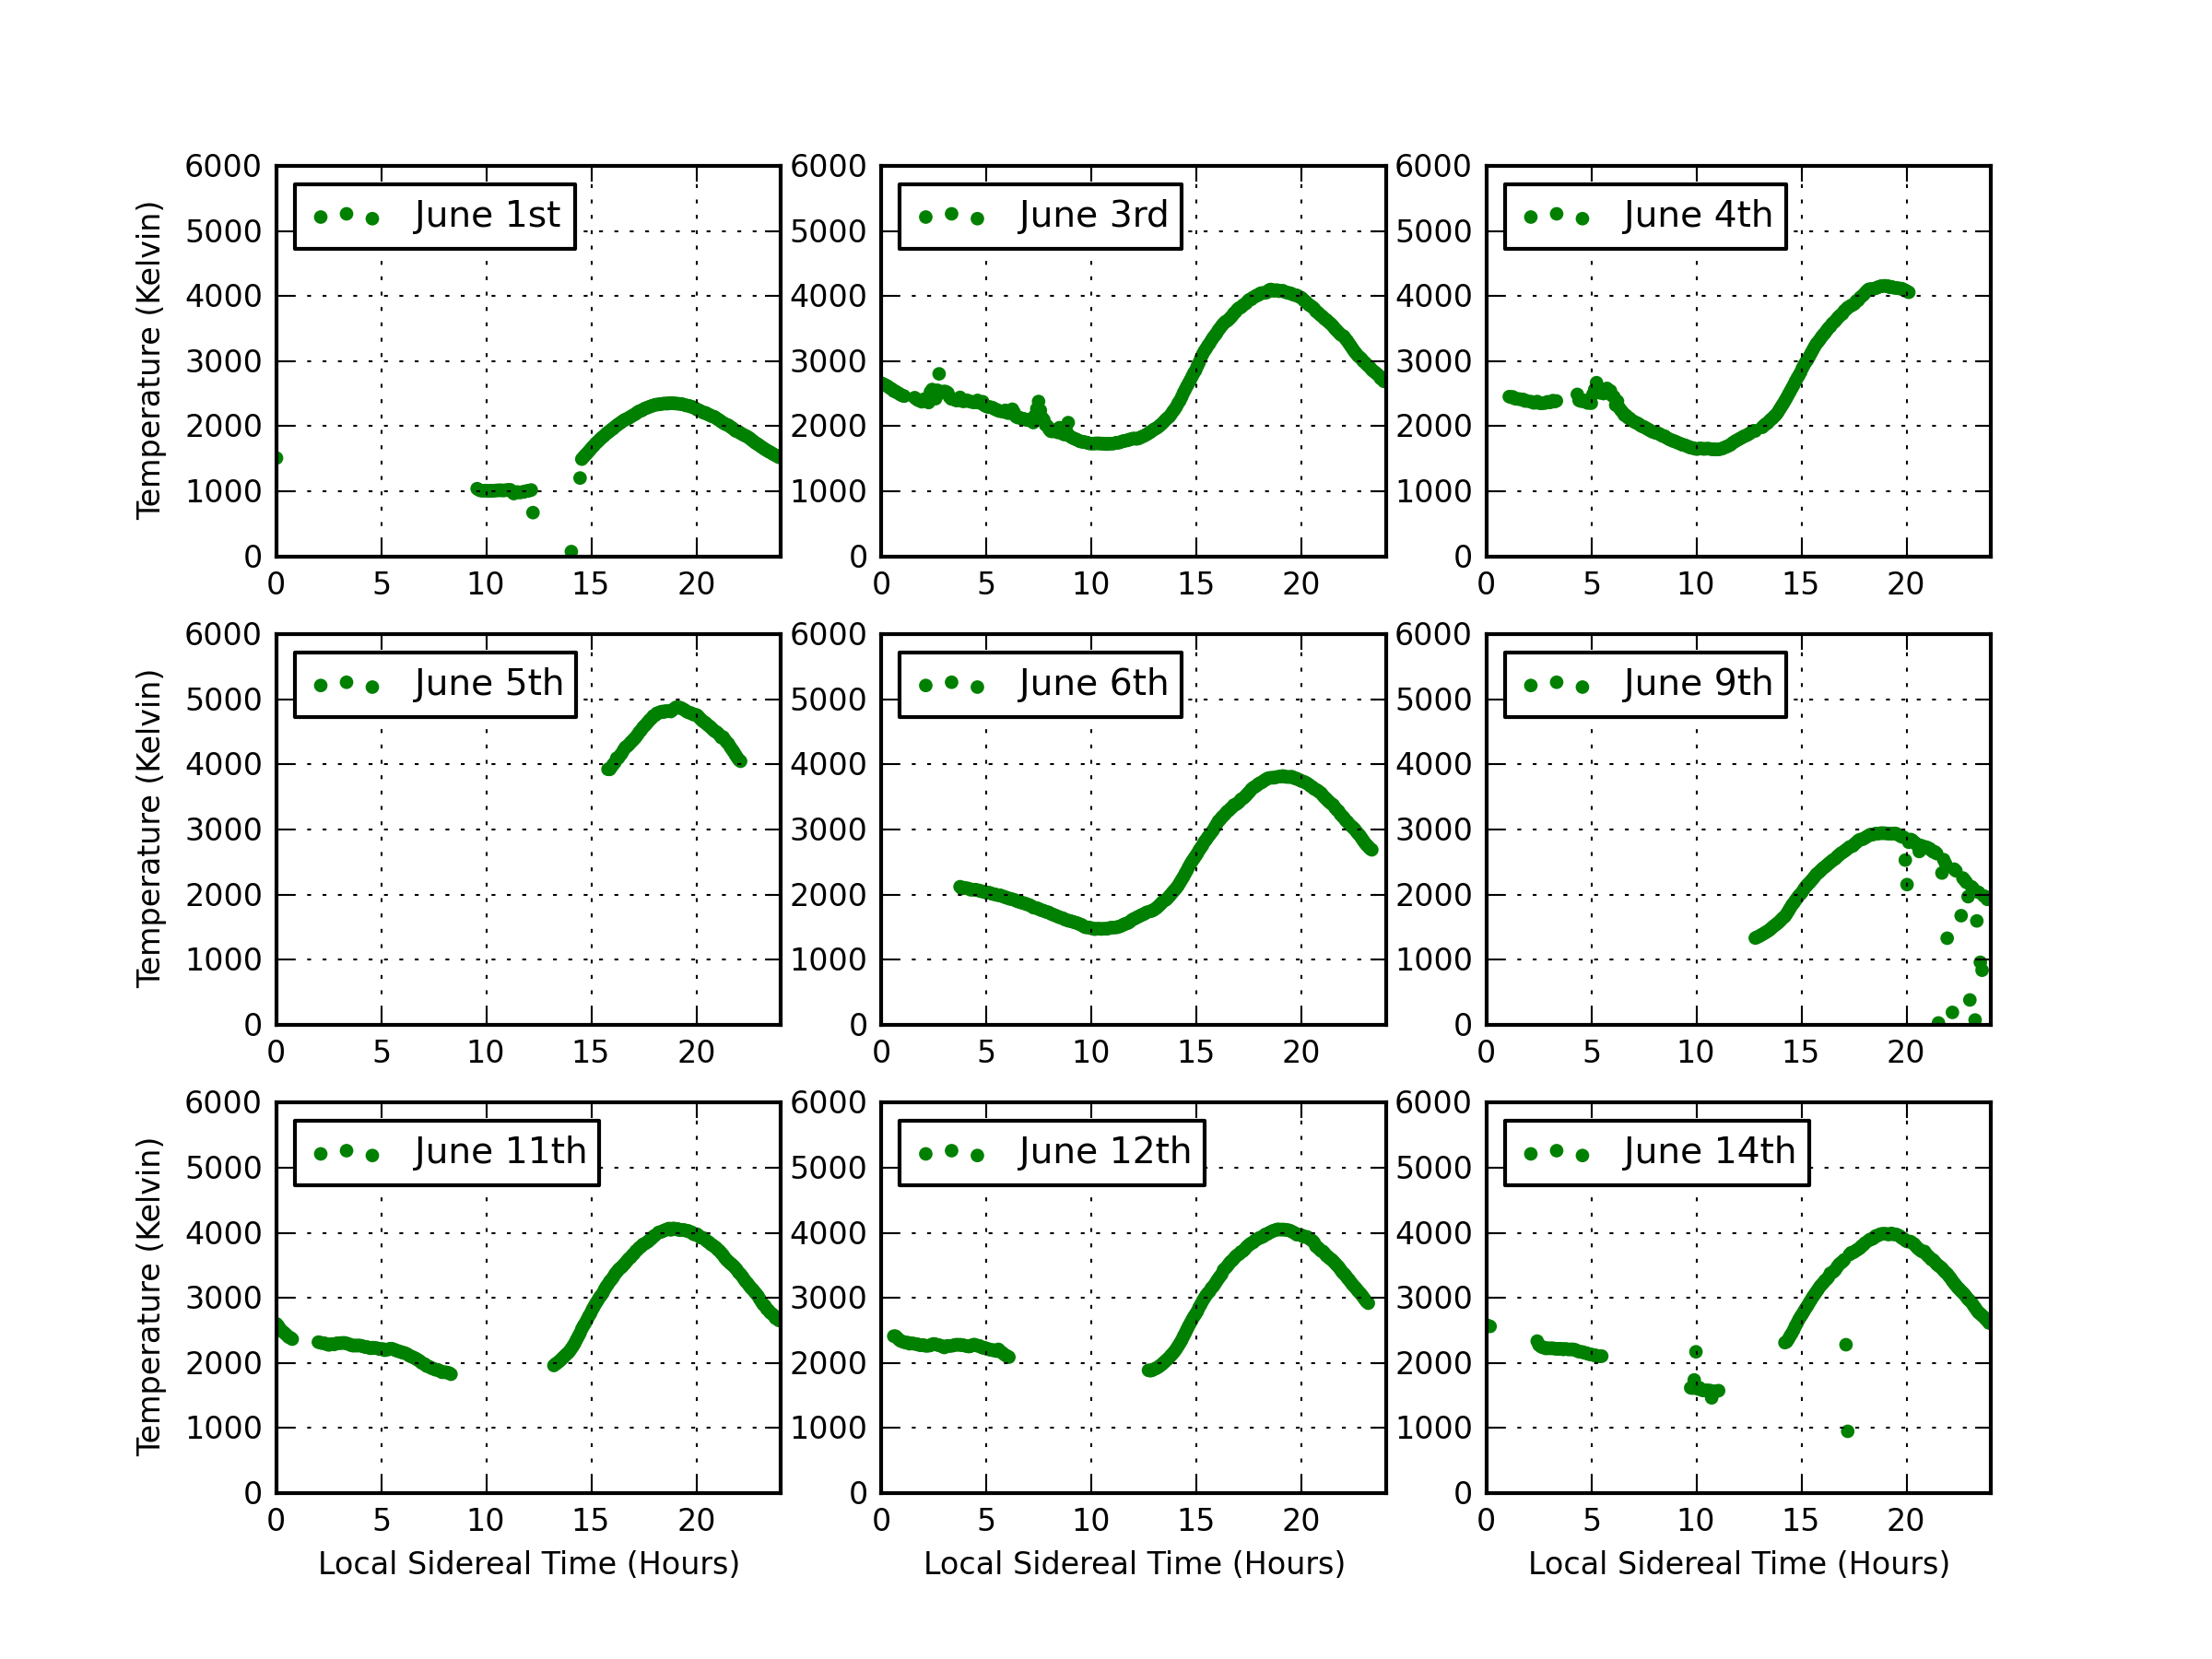
\includegraphics[width=0.95\linewidth]{Data_analysis/figures/Combined_Kdgsm_time_series.png}
\caption{Fits for $K_{\Delta GSM}$ calibration term for multiple days in June 2013 at 70 MHz. Days where a smaller percentage of the data is available have poorer fits. }
\label{Fig:Kdgsm_var}
\end{center}
\end{figure}

\subsubsection{Daily Variance with GSM Modelling ($K_{\Delta GSM}$)}\label{Sec:KGSM}

An alternative to calibration using the Johnson noise datasets is calibration using a source on the sky, which in our case is the Milky Way Galaxy. 

From our GSM model, we have an equation for the sky temperature ($T_{GSM}$), so our $P_{sky}$ can be calculated as:

\begin{equation}
T_{sky} = K_{\Delta GSM}*P_{sky} = T_{\Delta GSM}
\end{equation}

And $K_{\Delta GSM}$ can be calculated using:

\begin{equation}
K_{\Delta GSM} = \frac{T_{GSM}}{P_{sky}} = \frac{T_{GSM}* \eta}{P_{ant}-P_{short}}
\end{equation}

In order to maximize the accuracy of $T_{GSM}$, it is better to use the combination of data from a full sidereal day rather than a single time step and remove the time independent component of the data. A $\chi^2$ fitting can then be done  for each frequency independently to get a $K_{\Delta GSM}$ value for that frequency. The $\chi^2$ fit can be written as:

\begin{equation}
\chi^2(\nu) =  \sum_t \big [ \Delta T_{sky}(\nu,t) - \Delta T_{GSM}(\nu,t) \big ]^2
\end{equation}

where $\Delta T_{sky} (\nu, t) = T_{sky}(\nu,t)-\langle T_{sky} \rangle_{DAY} (\nu)$ and $\Delta T_{GSM} (\nu,t) = T_{GSM}(\nu,t)-\langle T_{GSM} \rangle_{DAY} (\nu)$. 

This calibration strategy can be considered analogous to the traditional radio calibration strategy, where the telescope points on and off the source. Once the fit has been calculated, it can be applied to the data (as shown in Figure \ref{Fig:Kdgsm}). 

In order for this calibration strategy to be successful, it is necessary to have the full day of data. When the calibration strategy is applied to a dataset where less than a full day of data is available, inaccuracies in the simulated beam or GSM model have a larger impact on the calibration. This can be seen in Figure \ref{Fig:Kdgsm_var}, where the magnitude of $K_{\Delta GSM}$ at a particular frequency is clearly different when less of the day's data is available. 

\begin{figure}[htb]
\centering
\begin{minipage}[b]{0.48\textwidth}
\centering
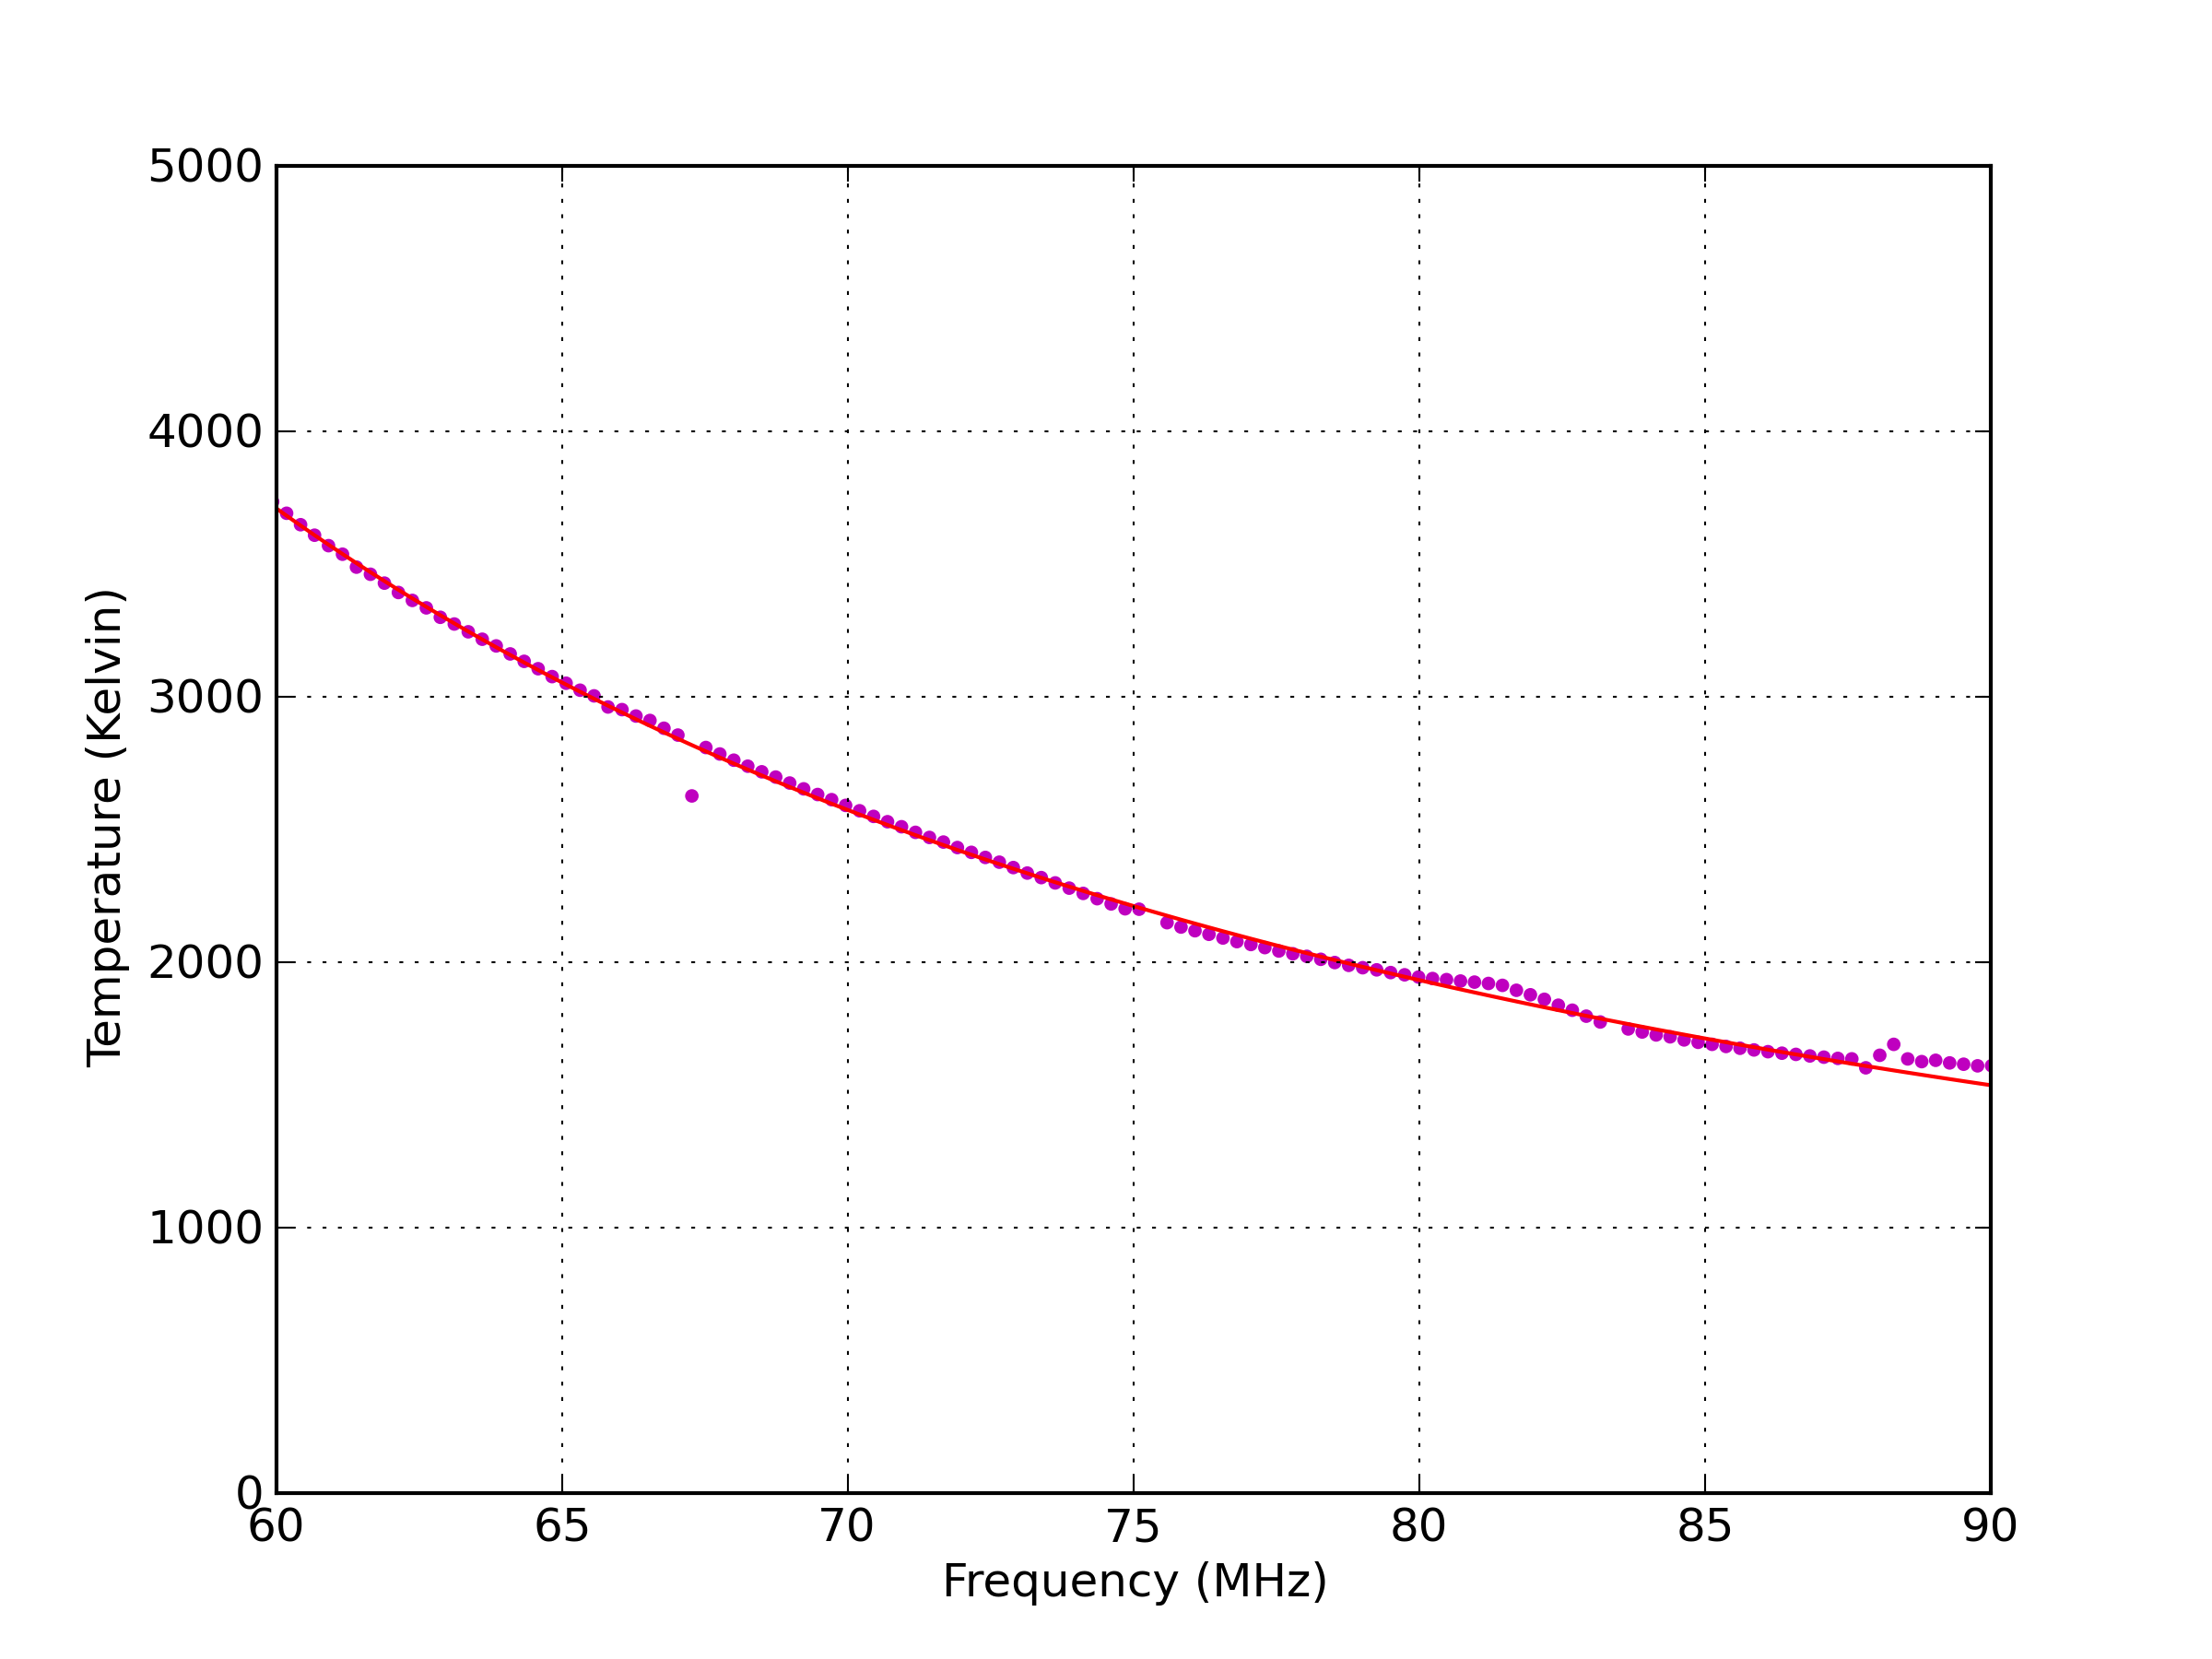
\includegraphics[width=0.95\linewidth]{Data_analysis/figures/June_04_Kdgsm_mean_fit.png}
\caption{Daily Mean of data from June 4th, 2013 calibrated using $K_{\Delta GSM}$, along with the foreground fit polynomial calculated for the data. }
\label{Fig:Kdgsm_mean}
\end{minipage}%
\begin{minipage}[b]{0.02\textwidth}
\hspace{1cm}
\end{minipage}%
\begin{minipage}[b]{0.48\textwidth}
\centering
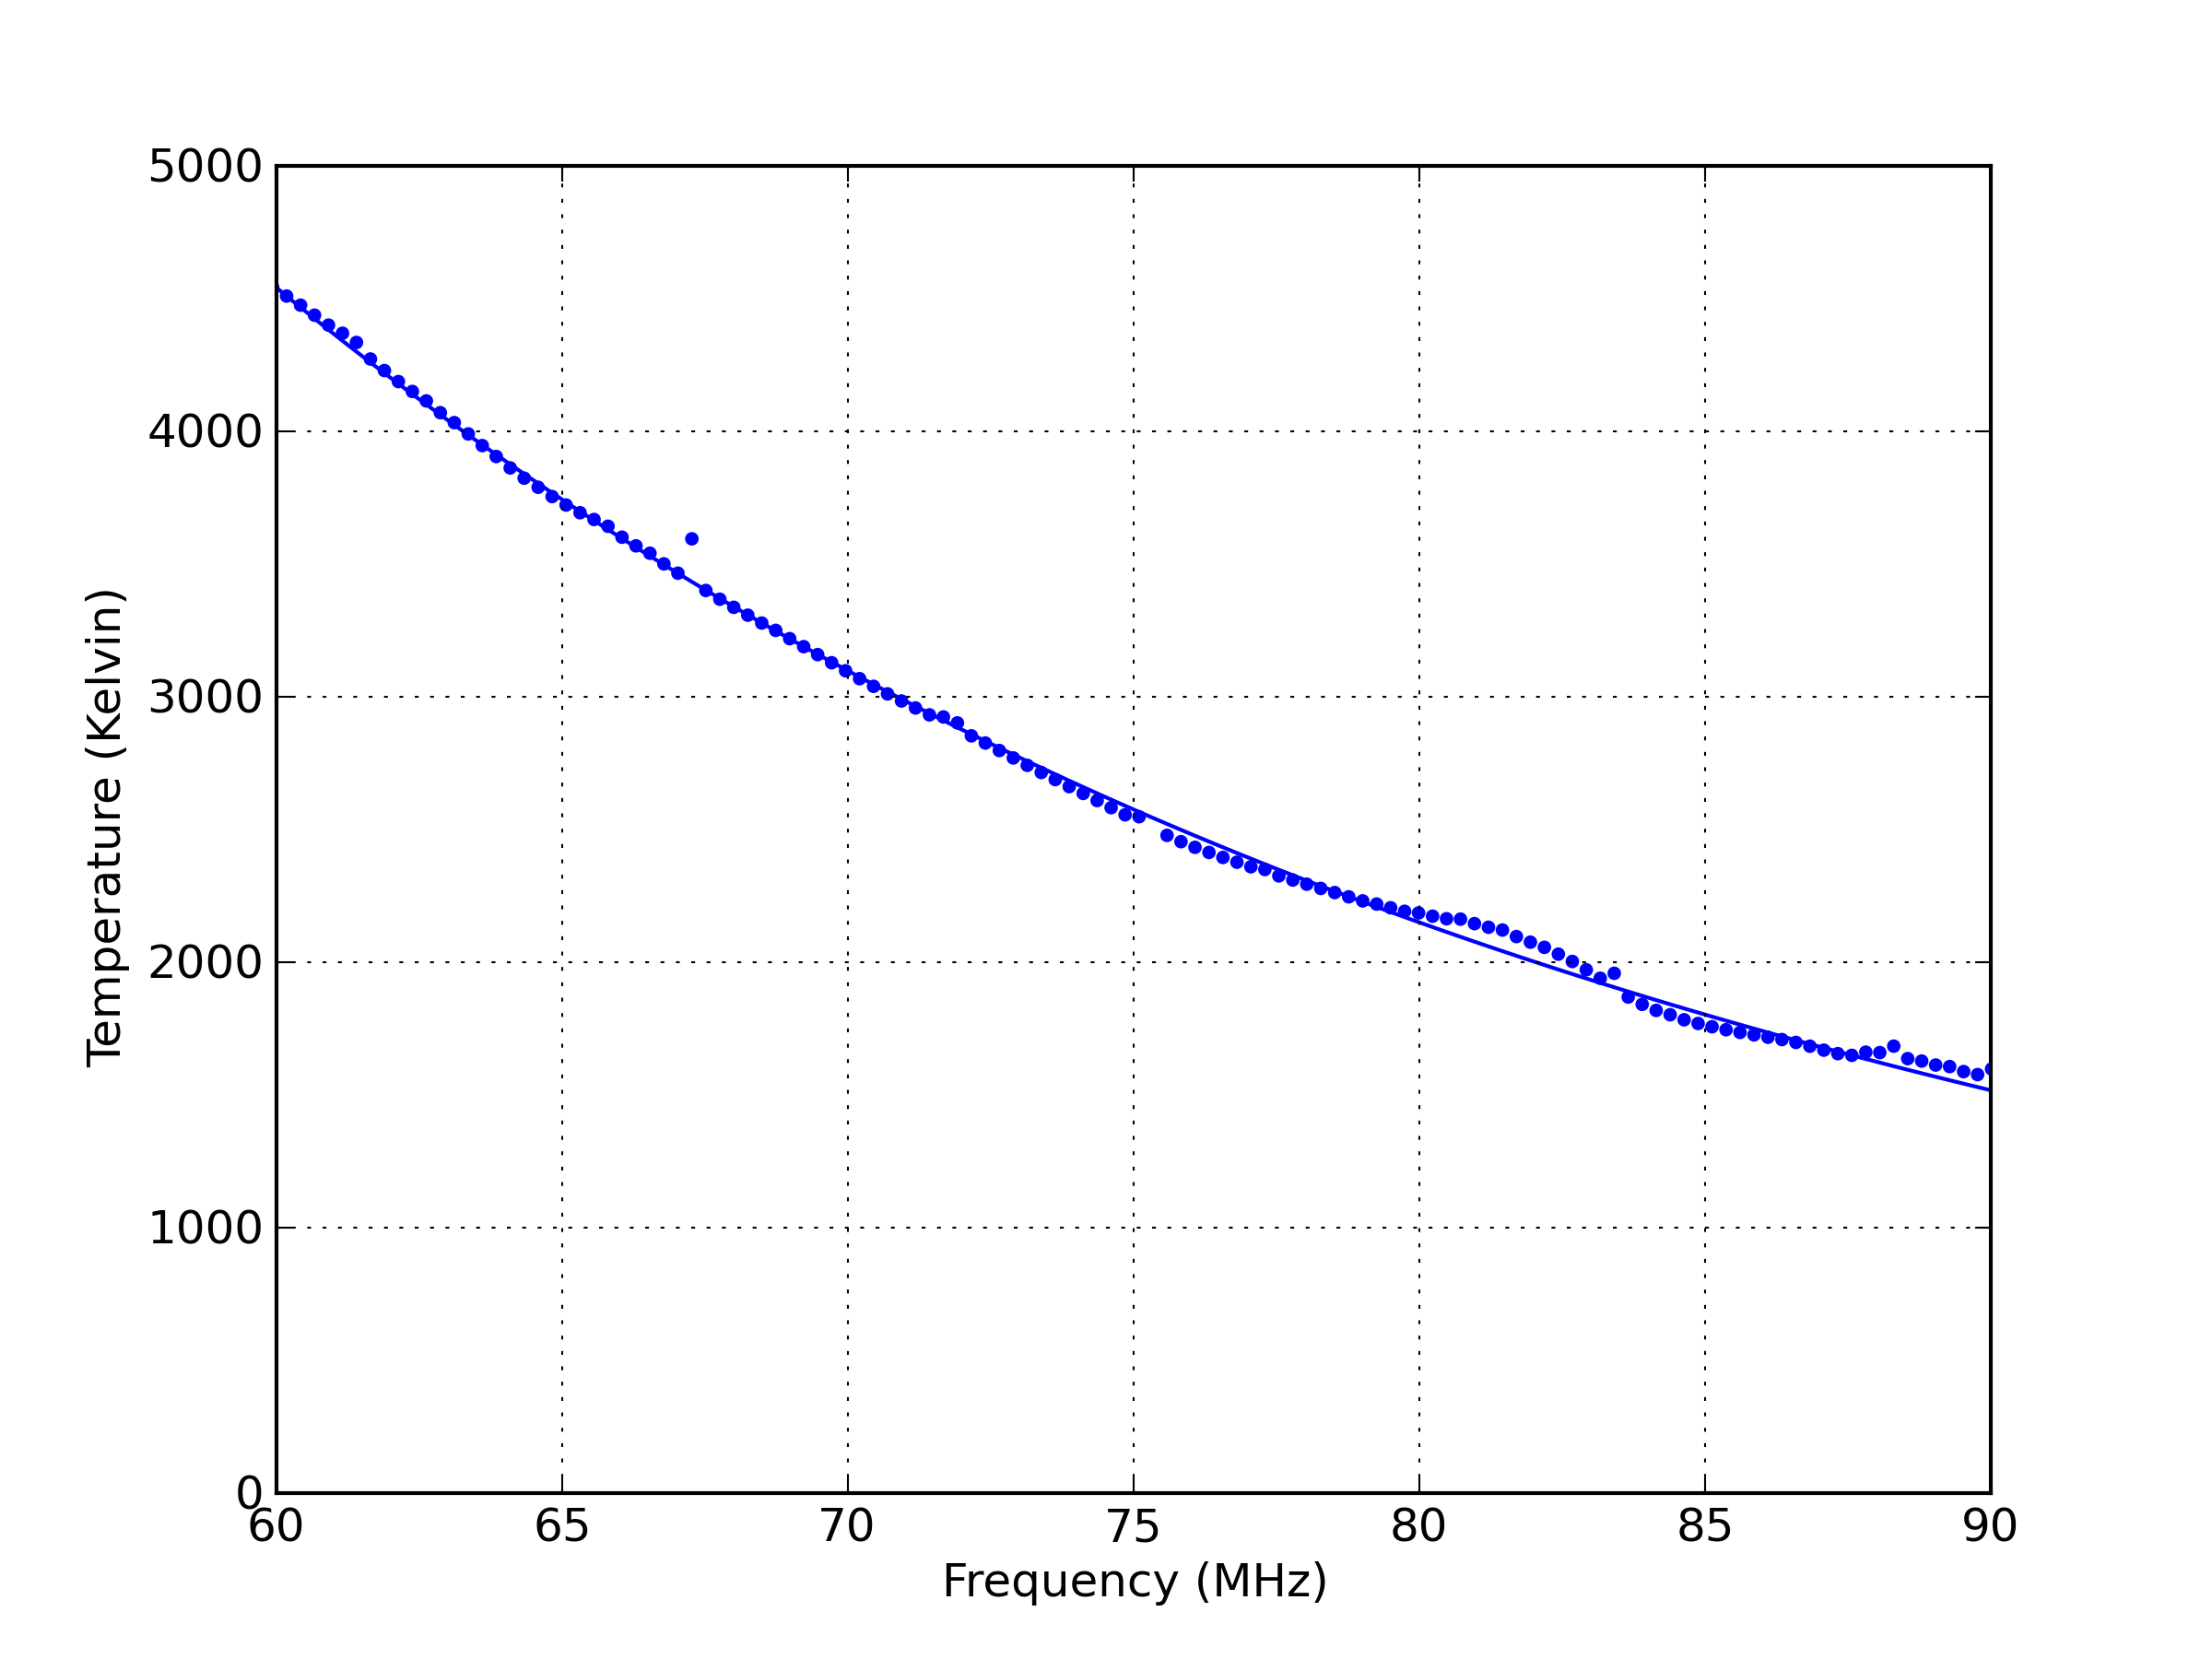
\includegraphics[width=0.95\linewidth]{Data_analysis/figures/June_04_Kt_mean_fit.png}
\caption{Daily Mean of data from June 4th, 2013 calibrated using $K_{JNC}$, along with the foreground fit polynomial calculated for the data. }
\label{Fig:Kjnc_mean}
\end{minipage}
\end{figure}



\section{Removing the Foregrounds}\label{Sec:fore}


\subsection{Polynomial Fitting}

Once the data has been calibrated, the Milky Way Galaxy and other foregrounds have to be removed to reveal the \cm structure. This removal is possible thanks to the simplicity of the galactic sky-averaged brightness temperature ($T_{GM}(\nu)$). 

\begin{equation}
T_{GM}(\nu) = \langle T_{sky}(\nu,t) \rangle_{DAY} - T_{\cm} (\nu) - T_{resid} (\nu)
\end{equation}

We can model $T_{GM} (\nu)$ as a simple polynomial of the form:

\begin{equation}
log_{10} T_{GM}(\nu) = \sum_{k=0}^n a_k \Big[ log_{10} \Big(\frac{\nu}{70 MHz}\Big) \Big]^k
\end{equation}

A n=2 polynomial captures the expected foreground brightness temperature at the log-center of the frequency band ($a_0$), a power law spectral shape ($a_1$), and a synchrotron self-absorption correction term ($a_2$). When we use the GSM calibration, the foreground values for the June 2013 data are $a_0 = 3.3826 \pm 0.1825$, $a_1 = -2.3747 \pm 0.3178$, and $a_2 = 0.3903 \pm 1.9351$. When we use the JNC calibration, the foreground values for the June 2013 data are $a_0 = 3.5186 \pm 0.0432$, $a_1 = -2.6205 \pm 0.0533$, and $a_2 = -2.5400 \pm 1.0962$. 

Some of the variance in the foreground fit parameters comes from the fact that the daily averages are calculated for different fractions of a full 24 period depending on the day selected. Additional variance is seen in the GSM calibration parameters due to the weakness of the calibration strategy when less tha a full day of data is observed. This was previously discussed in Section \ref{Sec:KGSM}.

Once we subtract this polynomial, we are left with residuals:

\begin{equation}
\Delta T (\nu) = T_{\cm}(\nu)+T_{resid}(\nu)
\end{equation}

Figures \ref{Fig:Kdgsm_mean} and \ref{Fig:Kjnc_mean} show the daily mean of one day of data from June 2013, along with its corresponding polynomial fit. 

\begin{figure}[htb]
\begin{center}
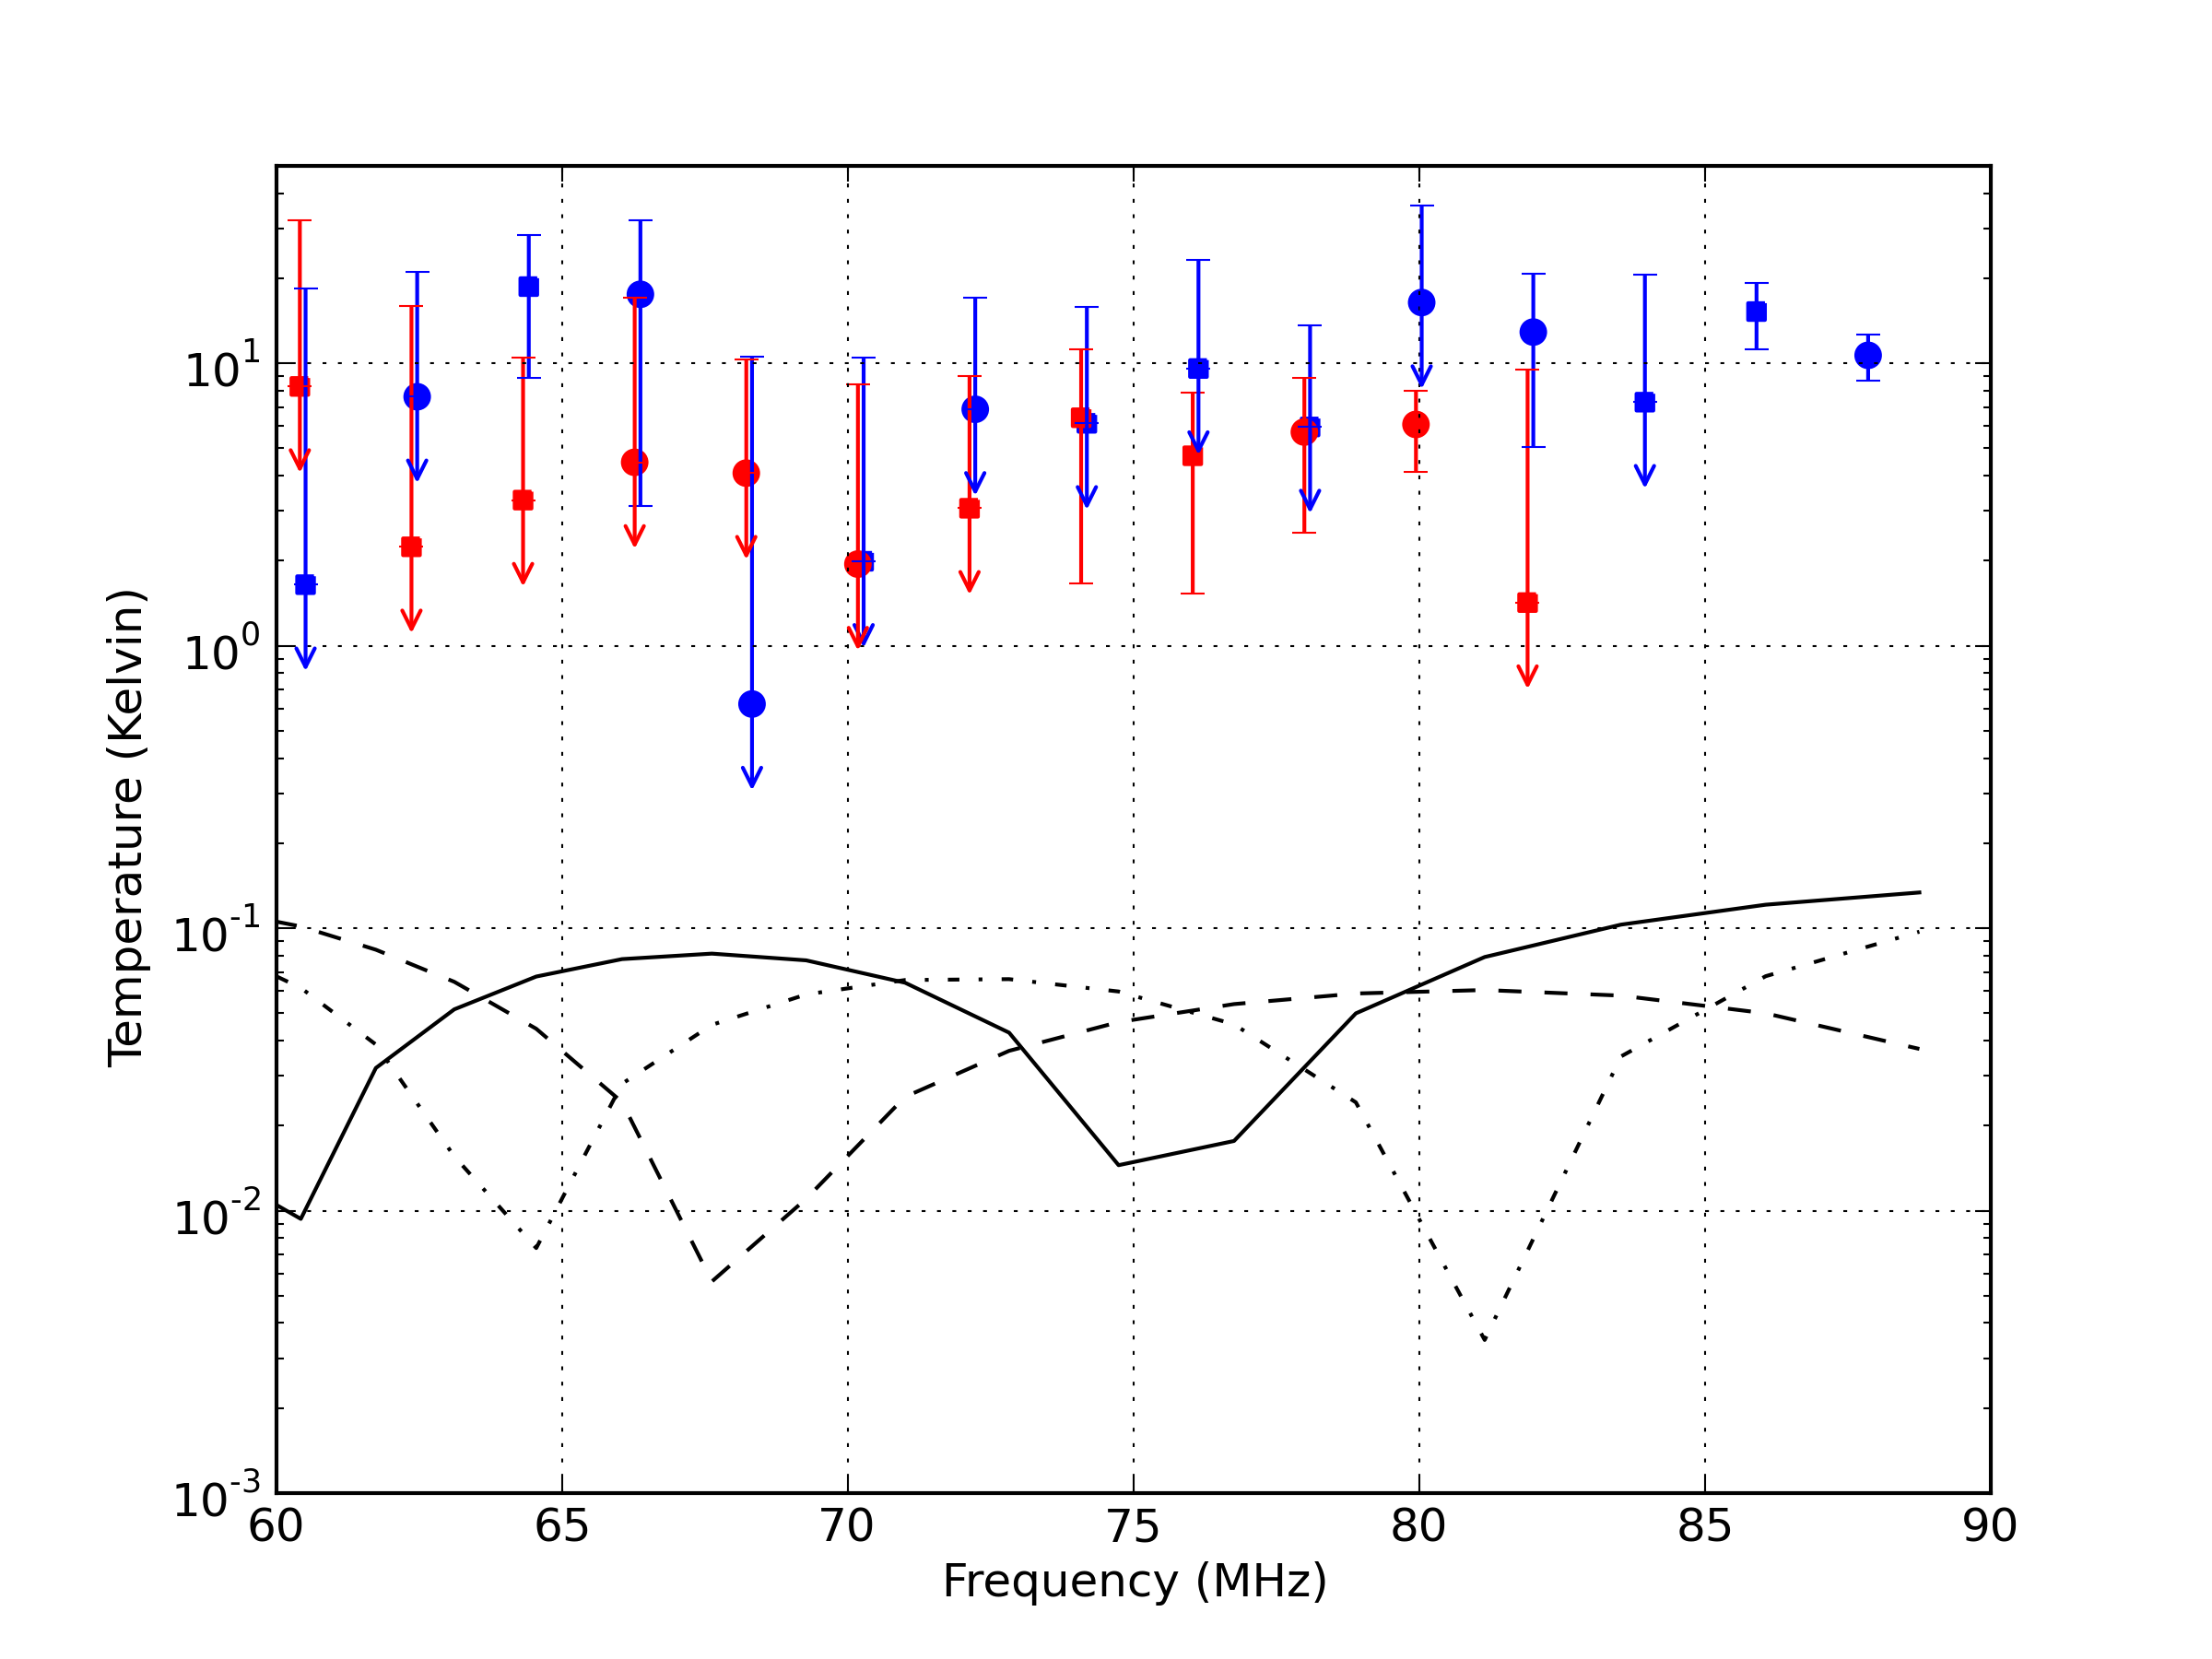
\includegraphics[width=0.95\linewidth]{Data_analysis/figures/joint_log_means.png}
\caption{Daily residuals and variance for data calibrated using either the Galaxy calibration (red) or Johnson Noise calibration (blue) compared to different models of the \cm signal (black). }
\label{Fig:resid}
\end{center}
\end{figure}


\subsection{Daily Residuals}

We calculate and apply the foreground fit separately for each daily mean, giving a distribution of residual data at each frequency. Measurement of the $T_{\cm}$ spectrum requires residuals whose dominant component is the \cm structure. Since the theoretical models of $T_{\cm}$ have a maximum structure $\sim 100 $mK, residuals must reach this limit for $T_{\cm}$ models to be constrained. The distributions of daily residuals from the June 2013 data are too large to constrain the theoretical models, as is shown in Figure \ref{Fig:resid}. 

These residuals are $\sim 1-10$K, which is much smaller than the foreground signal ($\sim 1000$K) at these frequencies. These residuals are the lowest published results in this frequency band and demonstrate the potential of the SCI-HI system for future measurements \cite{Voytek_2014}. 


\subsection{Frequency Limitations}

In order to achieve reasonable residuals, it was necessary to limit the frequency range of the analysis to avoid frequencies where $T_{resid}$ is large due to RFI from the SCI-HI system or other external sources. In the data collected in June 2013, the useable frequencies were limited to $\sim 60-85 MHz$. Below 60 MHz, there was additional large scale structure in the spectra, which may be due to either ionospheric impacts on the beam shape or inaccuracies in the simulated HIbiscus beam compared to the actual beam. Above 85 MHz there was contamination from both external FM signals and self-generated noise from the SCI-HI system. 

\begin{figure}[htb]
\begin{center}
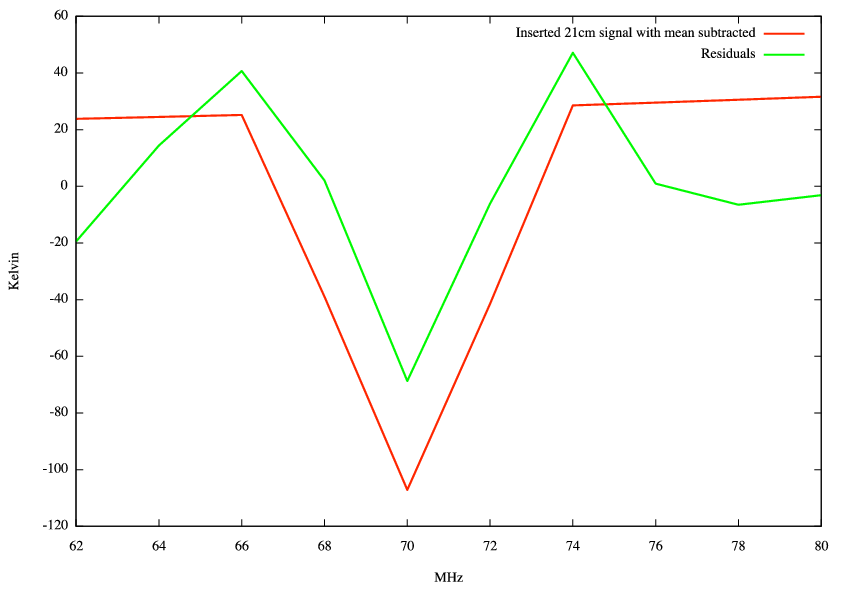
\includegraphics[width=0.9\linewidth]{Data_analysis/figures/100_K_21cm_signal.png}
\caption{Simulated \cm signal with 100 K magnitude (red) and residuals (green) ater calibration and foreground removal. }
\label{Fig:100K_sim}
\end{center}
\end{figure}



\section{\cm Signal Attenuation}

An important cross-check for any \cm measurement experiment is a simulation calibration measurement of signal attenuation \cite{paciga_2013}. This check is done by adding a simulated \cm signal to the raw data and then running the combination data through the signal pipeline. Figure \ref{Fig:100K_sim} shows what happens when a simulated \cm signal, magnified to 100 K to make it easy to identify, is run through the analysis pipeline. 

Because the \cm signal is constant with time with complex structure in frequency, there is minimal signal attenuation caused by the calibration strategy and foreground removal process. 



\section{Ionospheric impacts}

All of the data analysis above was done assuming no ionospheric impacts on the data. However, Figures \ref{Fig:day_TEC_NA} and \ref{Fig:night_TEC_NA} indicate that there should be some ionospheric impact on the data, particularly during the daytime hours. 


\subsection{Refraction} 

Since ionospheric refraction affects the direction of sky signals, refraction will lead to inaccuracies in $T_{GSM}$, particularly at large $\theta$. These inaccuracies will propogate into the $K_{\Delta GSM}$ calibration factor. 

Refraction will also affect the signal regardless of calibration strategy. This is because the foreground subtraction strategy relies on frequency independent sky area coverage. Any variance in the sky area coverage at different frequencies will lead to structure in the spectrum. Since the HIbiscus sky coverage is designed to be constant in frequency with no ionospheric refraction, the refracted beam will not be constant with frequency. 


\subsection{Absorption}

Frequency dependent absorption can also introduce additional structure to the mean signal ($\langle T_{sky}(\nu,t) \rangle_{DAY}$). If $TEC$ is constant for the data, then the structure will simply add an additional term in $T_{GM}$. But if $TEC$ is variable, then the absorption structure can be quite complex. 


\subsection{Ionospheric Structure}

The residual levels shown in Figure \ref{Fig:resid} set a maximum level for the total ionospheric impact in the frequency band of ($\sim 60-85 MHz$) at $\sim 1-10 K$.  Ionospheric impact may be larger if the $a_2$ term defined in the $T_{GM}$ polynomial is caused by the ionosphere rather than Galactic structure. This can be quantified using the time dependence of $a_2$. If $a_2$ is from the ionosphere it should be $\propto TEC$. On the other hand, if $a_2$ is from Galactic structure then $a_2$ should depend on the part of the Milky Way Galaxy currently in the beam. 

Self-generated noise and time gaps in the SCI-HI data from June 2013 make it difficult to run the ionospheric analysis, but data collected with an improved system may make this distinction possible. 
